\documentclass[12pt,a4paper]{report}
\usepackage{fontspec}
\setmainfont{Times New Roman}
\usepackage{geometry}
\geometry{margin=1in}
\usepackage{graphicx}
\usepackage{booktabs}
\usepackage{float}
\usepackage{longtable}
\usepackage{array}
\usepackage{caption}
\usepackage{hyperref}
\usepackage{setspace}
\usepackage{amsmath}
\usepackage{tocloft}
\onehalfspacing
\setlength{\parskip}{0.45em}
\setlength{\parindent}{1.2em}

\title{Dự báo nhu cầu bán lẻ có xét đến stockout trên FreshRetailNet-50K}
\author{}
\date{}

\begin{document}
\pagenumbering{roman}
\maketitle

\begin{abstract}
Báo cáo này trình bày một pipeline stockout-aware demand forecasting cho FreshRetailNet-50K. Thay vì dự báo trực tiếp observed sales, đồ án recover latent demand trong các giờ stockout, aggregate lên daily demand, rồi forecast tổng nhu cầu 7 ngày tiếp theo. Trọng tâm của báo cáo là tính đúng đắn theo thời gian, kiểm soát imputation, so sánh với benchmark và diễn giải business.
\end{abstract}

\tableofcontents
\listoffigures
\listoftables
\clearpage
\pagenumbering{arabic}

\section{Giới thiệu và động lực kinh doanh}

Bài toán trong đồ án này không chỉ là dự báo doanh số bán được trong tương lai. Trong bán lẻ, doanh số quan sát được có thể bị giới hạn bởi tồn kho: khi một sản phẩm hết hàng, số lượng bán được thấp không phản ánh đầy đủ nhu cầu thật. Nếu doanh nghiệp dùng trực tiếp doanh số quan sát được để dự báo, hệ thống có thể học nhầm rằng nhu cầu thấp, từ đó nhập hàng ít hơn, tiếp tục gây stockout trong các kỳ sau. Đây là vòng lặp vận hành quan trọng:

\begin{center}
\texttt{stockout -> observed sales thấp -> forecast thấp -> nhập ít -> tiếp tục stockout}
\end{center}

Vì vậy, câu hỏi nghiên cứu của đồ án được đặt lại theo hướng gần với nghiệp vụ hơn: làm thế nào để dự báo nhu cầu bán lẻ khi dữ liệu doanh số bị kiểm duyệt bởi trạng thái hết hàng? Thay vì chỉ dự báo \textit{observed sales}, báo cáo này xây dựng pipeline dự báo \textit{recovered demand}, tức nhu cầu được hiệu chỉnh sau khi xét đến stockout.

\subsection{Câu hỏi nghiên cứu}

Báo cáo tập trung vào bốn câu hỏi chính. Thứ nhất, dữ liệu FreshRetailNet-50K có các pattern thời gian nào quan trọng cho dự báo, đặc biệt là seasonality theo giờ, theo ngày và theo tuần? Thứ hai, stockout làm observed sales bị kiểm duyệt ở mức độ nào và có cần latent demand recovery hay không? Thứ ba, recovery demand có làm tổng nhu cầu tăng quá mức hay không, và làm sao kiểm soát rủi ro imputation? Thứ tư, sau khi recover demand, mô hình forecasting nào phù hợp nhất cho bài toán daily next-7-day demand?

\subsection{Đóng góp chính của đồ án}

Đóng góp của đồ án được hiểu theo nghĩa thực nghiệm và ứng dụng, không phải đề xuất một thuật toán deep learning hoàn toàn mới. Điểm mới nằm ở cách framing bài toán, cách xử lý stockout và cách biến kết quả forecast thành insight vận hành.

\begin{table}[H]
\centering
\caption{Tóm tắt contribution của đồ án}
\label{tab:contribution-summary}
\resizebox{\linewidth}{!}{%
\begin{tabular}{lll}
\toprule
Nhóm đóng góp & Nội dung thực hiện & Ý nghĩa \\
\midrule
Problem framing & Chuyển từ forecast observed sales sang forecast recovered demand & Gần hơn với quyết định replenishment \\
Data treatment & Recover latent demand ở cấp hourly rồi aggregate lên daily & Giữ đúng nơi stockout xuất hiện nhưng trả forecast ở cấp vận hành \\
Leakage control & Expanding-window recovery theo block tuần & Không dùng ngày tương lai để recover quá khứ \\
Imputation control & Calibration, cap q90, pseudo-stockout validation, sensitivity & Tránh để imputation làm phình tổng demand quá mức \\
Modeling insight & So sánh observed-sales, recovered-demand, seasonal naive và hybrid & Chứng minh seasonality tuần là baseline rất mạnh \\
Business insight & Đo mức demand bị che bởi stockout và tác động lên forecast & Hỗ trợ nhận diện SKU/store có rủi ro thiếu hàng \\
\bottomrule
\end{tabular}
}
\end{table}

Nói ngắn gọn, contribution chính không phải là ``dùng LightGBM'' hay ``vẽ thêm nhiều biểu đồ''. Contribution chính là xây dựng một quy trình forecast có xét cơ chế stockout-censoring: observed sales bị kiểm duyệt, demand được recover có kiểm soát, sau đó forecast được đánh giá trên demand proxy phù hợp hơn cho vận hành.

\subsection{Phạm vi và điều không claim}

Đồ án không claim rằng recovered demand là ground truth tuyệt đối. Đây là proxy được ước lượng từ dữ liệu non-stockout và được kiểm soát bằng các kiểm tra aggregate/sensitivity. Đồ án cũng không claim đánh bại mọi mô hình deep learning hiện đại. Mục tiêu là một pipeline chặt chẽ, tái lập được, có benchmark rõ ràng và diễn giải được về mặt business.

\subsection{Kết quả chính ở mức tổng quan}

Sample thí nghiệm dùng 0.1 theo cấp \texttt{series\_id}, gồm 11640000 quan sát hourly và 5000 chuỗi, từ 2024-03-28 00:00:00 đến 2024-07-02 23:00:00. Tỷ lệ stockout row khoảng 24.65\%. Sau recovery, recovered demand tăng khoảng 10.68\% so với observed sales, cho thấy observed sales có khả năng đang understated demand do hết hàng.

Khi đánh giá trên recovered latent demand proxy, observed-sales LightGBM đạt WAPE 24.42\%; recovered-demand LightGBM giảm xuống 20.28\%. Seasonal naive 7-day đạt 19.85\%, cho thấy seasonality tuần rất mạnh. Mô hình kết luận cuối là Recovered seasonal-ML hybrid, đạt WAPE 19.67\%.

\section{Dữ liệu và tiền xử lý}

\subsection{Nguồn dữ liệu}

FreshRetailNet-50K là bộ dữ liệu bán lẻ nhiều chuỗi, trong đó mỗi chuỗi tương ứng với một tổ hợp cửa hàng--sản phẩm--thành phố. Dữ liệu gốc gồm các file \texttt{train.parquet} và \texttt{eval.parquet}. Điểm đặc biệt của bộ dữ liệu là ngoài sales, dữ liệu còn chứa trạng thái tồn kho theo giờ thông qua \texttt{hours\_stock\_status}, giúp phân biệt giai đoạn bán thấp vì nhu cầu thấp và giai đoạn bán thấp vì hết hàng.

\subsection{Tạo định danh chuỗi}

Biến \texttt{series\_id} được tạo từ \texttt{city\_id}, \texttt{store\_id} và \texttt{product\_id}. Việc tạo định danh này giúp mọi phép lag, rolling và split được thực hiện đúng theo từng chuỗi, không trộn thông tin giữa các sản phẩm hoặc cửa hàng khác nhau.

\subsection{Bung dữ liệu daily thành hourly}

Dữ liệu sale theo ngày được bung thành hourly bằng \texttt{hours\_sale}. Trạng thái stockout theo giờ được lấy từ \texttt{hours\_stock\_status}. Việc giữ cấp hourly là cần thiết vì stockout xảy ra theo giờ; nếu aggregate trực tiếp lên daily trước khi recover, ta có thể làm mất thông tin về thời điểm hết hàng trong ngày.

\subsection{Lấy sample theo series}

Đồ án không yêu cầu chạy full data. Vì vậy, sample 10\% được lấy ở cấp \texttt{series\_id}, giữ nguyên toàn bộ dòng thời gian của các chuỗi được chọn. Cách lấy sample này tốt hơn random row sampling vì không phá vỡ cấu trúc thời gian và không tạo chuỗi bị đứt đoạn.


\begin{table}[H]
\centering
\caption{Tóm tắt chất lượng dữ liệu}
\label{tab:long-data-quality}
\resizebox{0.82\linewidth}{!}{%
\begin{tabular}{ll}
\toprule
Metric & Value \\
\midrule
Sample fraction & 0.1 \\
Number of rows & 11640000 \\
Number of series & 5000 \\
Number of stores & 866 \\
Number of products & 516 \\
Number of cities & 18 \\
Start date & 2024-03-28 00:00:00 \\
End date & 2024-07-02 23:00:00 \\
Frequency & Hourly rows expanded from hours\_sale and hours\_stock\_status \\
Missing dt count & 0 \\
Duplicate rows & 0 \\
Missing sale\_amount & 0 \\
Stockout rate & 0.24667061855670103 \\
Average sale\_amount & 0.04194150120019913 \\
Median sale\_amount & 0.0 \\
\bottomrule
\end{tabular}
}
\end{table}


\subsection{Split theo thời gian}

Tất cả các bước đánh giá đều dùng split theo thời gian, không dùng random split. Với dữ liệu hourly, validation gồm 7 ngày và test gồm 14 ngày cuối. Với bài toán daily next-7-day forecasting, báo cáo lưu thêm split theo forecast origin để làm rõ ngày dự báo và target window tương ứng.


\begin{table}[H]
\centering
\caption{Split hourly theo thời gian}
\label{tab:long-hourly-split}
\resizebox{0.82\linewidth}{!}{%
\begin{tabular}{lllll}
\toprule
Split & Start date & End date & Rows & Series \\
\midrule
Train & 2024-03-28 & 2024-06-10 23:00:00 & 9000000 & 5000 \\
Validation & 2024-06-11 & 2024-06-17 23:00:00 & 840000 & 5000 \\
Test & 2024-06-18 & 2024-07-01 23:00:00 & 1680000 & 5000 \\
\bottomrule
\end{tabular}
}
\end{table}



\begin{table}[H]
\centering
\caption{Split daily forecasting theo forecast origin}
\label{tab:long-daily-split}
\resizebox{\linewidth}{!}{%
\begin{tabular}{lllllll}
\toprule
Split & Origin start & Origin end & Target window start & Target window end & Rows & Series \\
\midrule
Train & 2024-03-28 & 2024-06-03 & 2024-03-29 & 2024-06-10 & 340000 & 5000 \\
Validation & 2024-06-04 & 2024-06-10 & 2024-06-05 & 2024-06-17 & 35000 & 5000 \\
Test & 2024-06-11 & 2024-06-24 & 2024-06-12 & 2024-07-01 & 70000 & 5000 \\
\bottomrule
\end{tabular}
}
\end{table}

\section{Phân tích khám phá dữ liệu}

\subsection{Aggregate sales và stockout}

Hai hình đầu tiên cho thấy bức tranh tổng quát của dữ liệu: aggregate observed sales theo thời gian và stockout rate theo thời gian. Đây là hai đồ thị quan trọng nhất để motivate bài toán. Nếu chỉ nhìn aggregate sales, các giai đoạn giảm bán có thể bị hiểu là demand giảm. Nhưng khi đặt cạnh stockout rate, ta thấy cần phân biệt giữa demand thấp và availability thấp.


\begin{figure}[H]
    \centering
    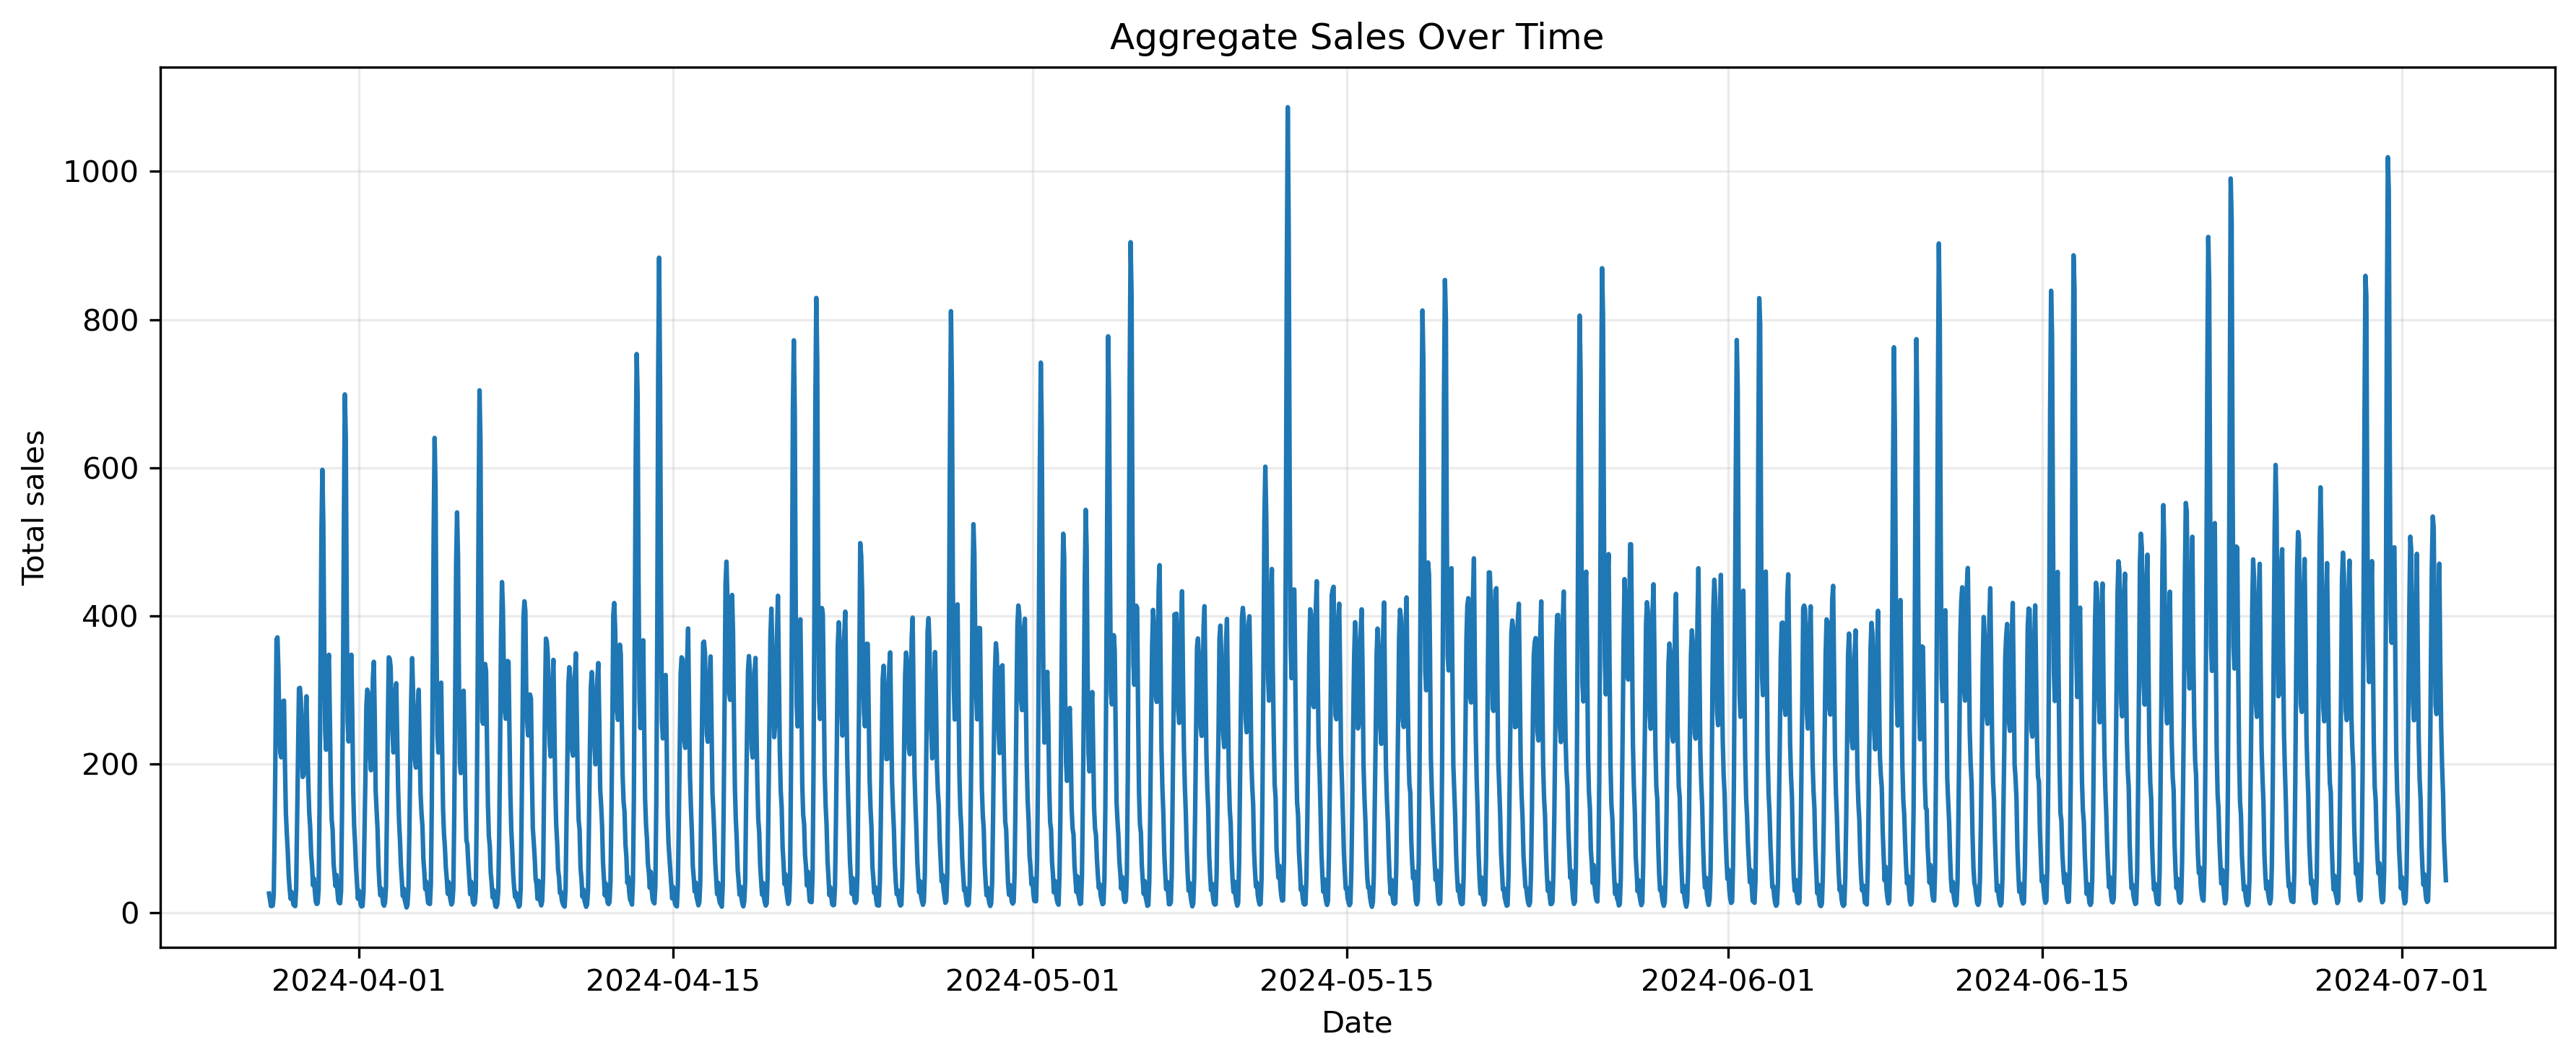
\includegraphics[width=0.92\linewidth]{figures/aggregate_sales_over_time.png}
    \caption{Tổng observed sales theo giờ.}
    \label{fig:long-aggregate-sales}
\end{figure}



\begin{figure}[H]
    \centering
    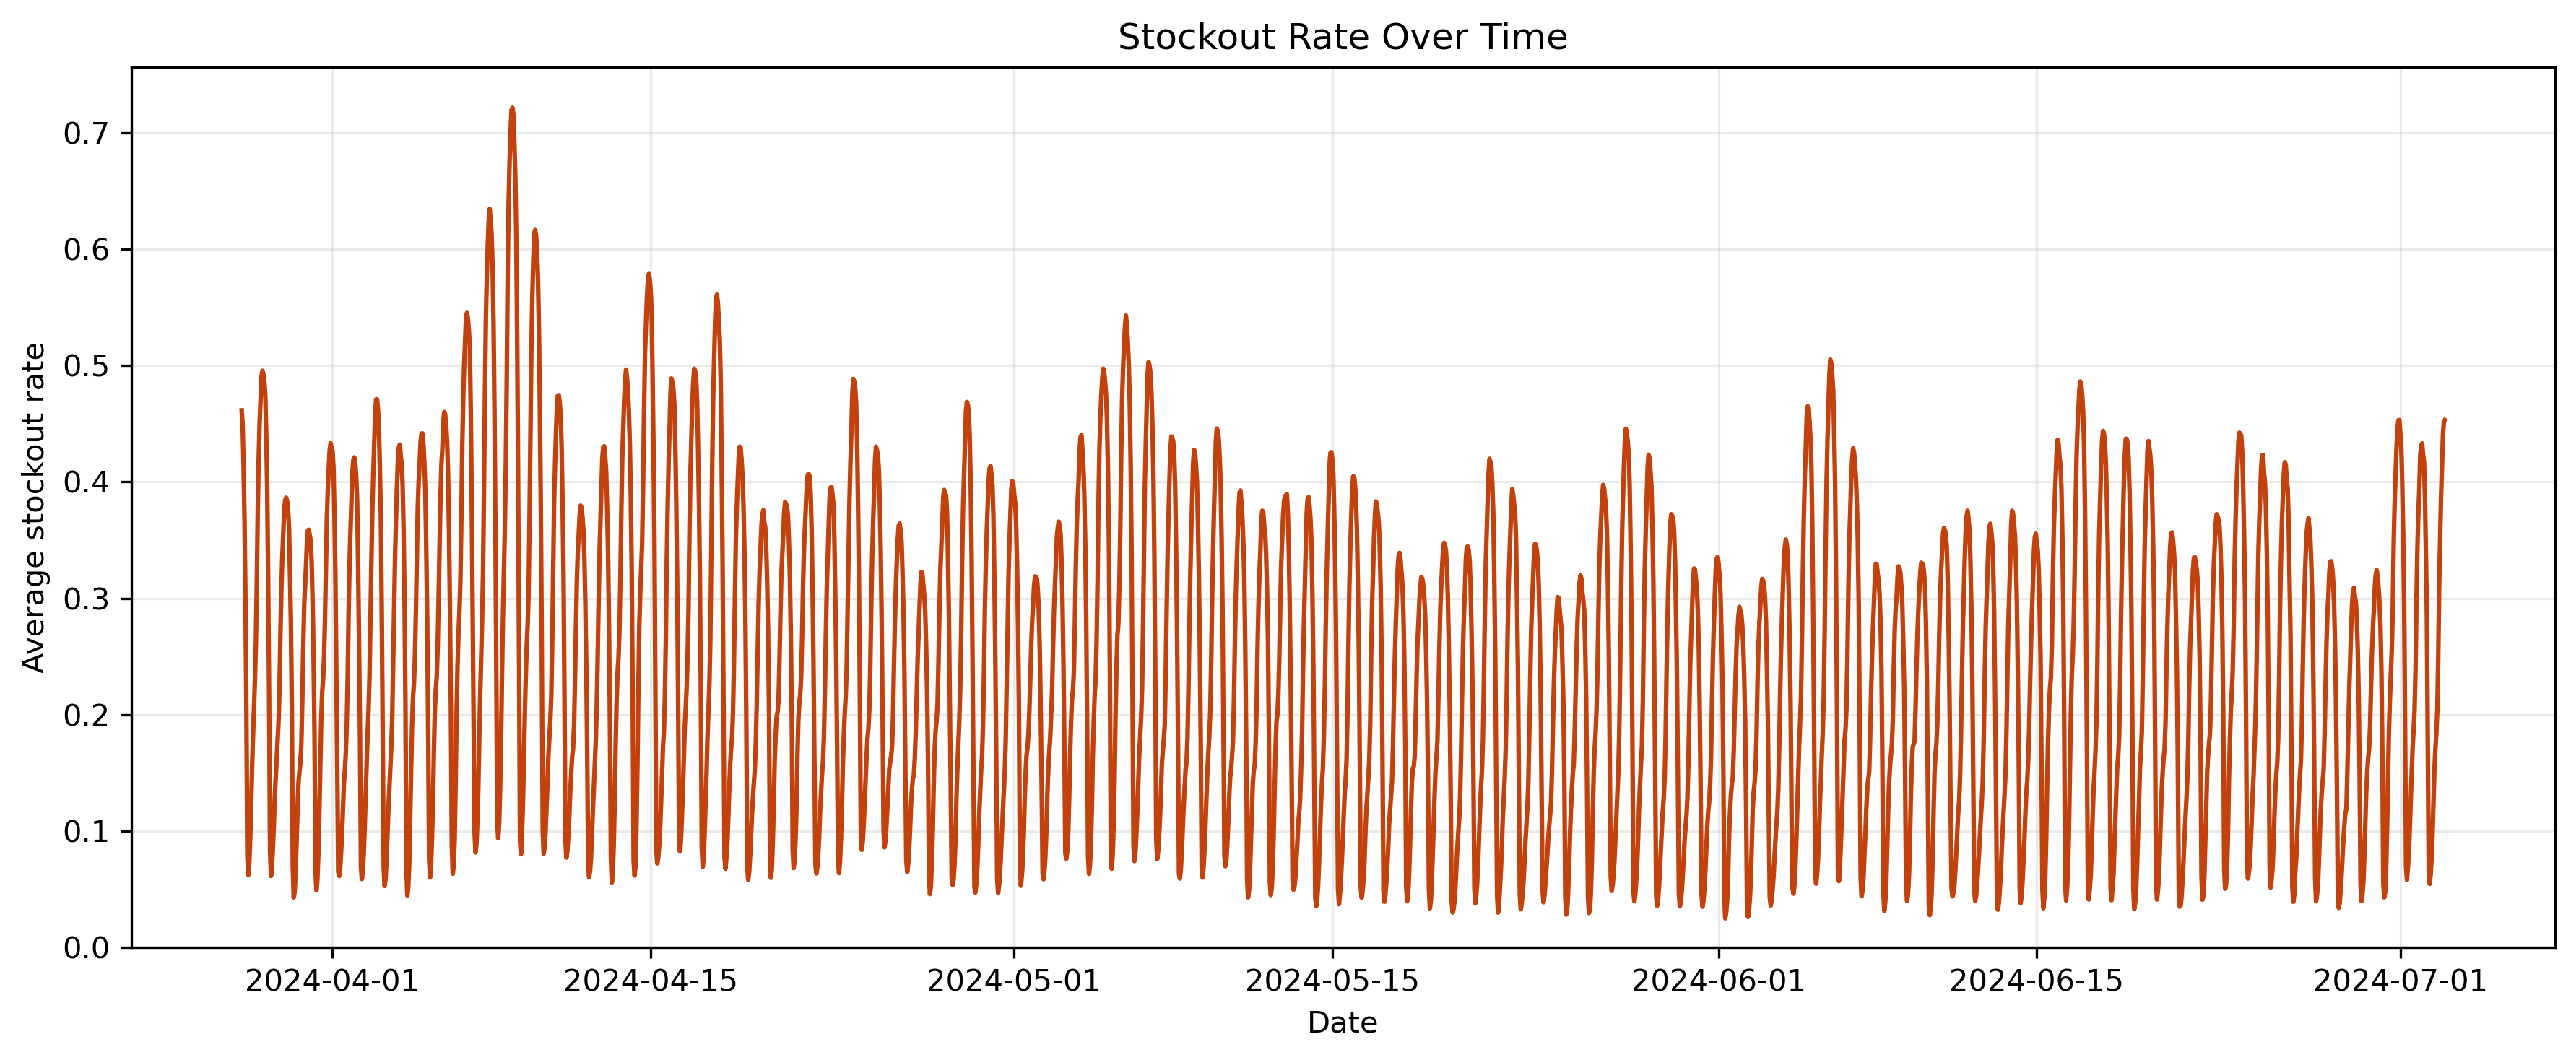
\includegraphics[width=0.92\linewidth]{figures/stockout_rate_over_time.png}
    \caption{Tỷ lệ stockout theo giờ.}
    \label{fig:long-stockout-rate}
\end{figure}


\subsection{Phân phối sales}

Phân phối sale amount cho thấy dữ liệu bán lẻ rất thưa, nhiều giá trị nhỏ và zero, đồng thời có các spike lớn. Đây là lý do không dùng MAPE đơn thuần làm metric chính; WAPE, MAE và RMSE phù hợp hơn vì ổn định hơn khi dữ liệu có nhiều zero.


\begin{figure}[H]
    \centering
    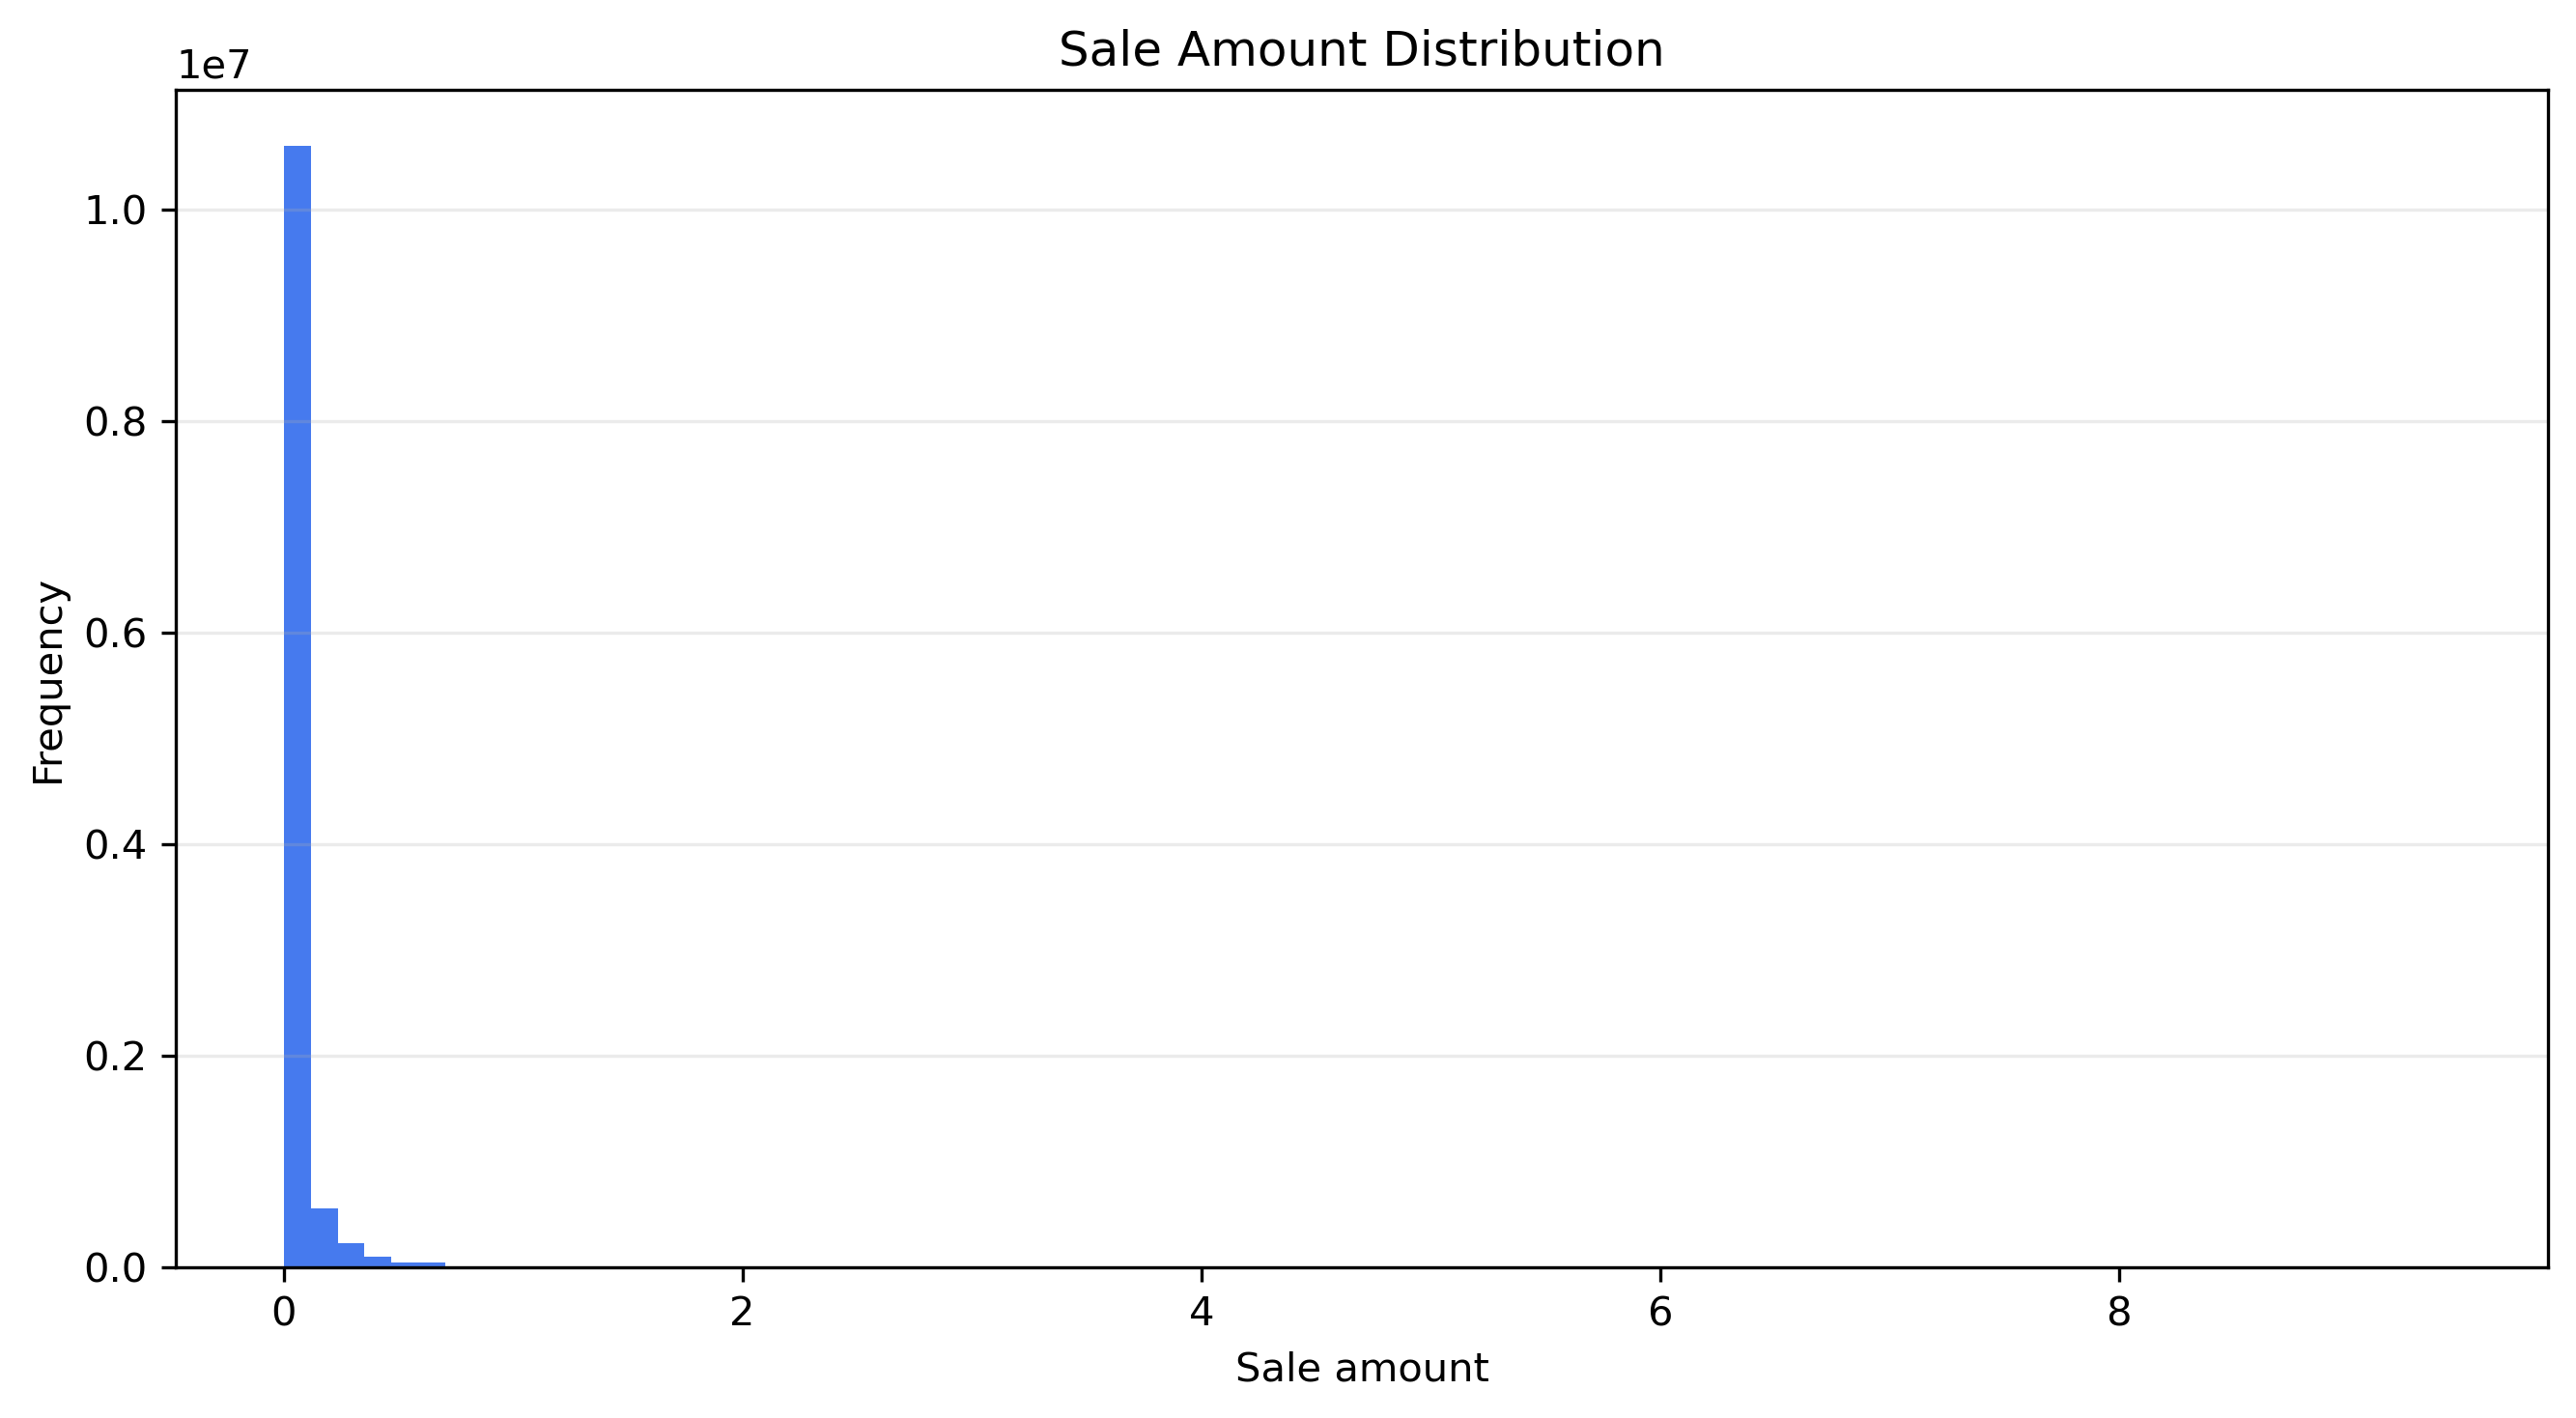
\includegraphics[width=0.78\linewidth]{figures/sale_amount_distribution.png}
    \caption{Phân phối sale amount hourly.}
    \label{fig:long-sale-dist}
\end{figure}



\begin{figure}[H]
    \centering
    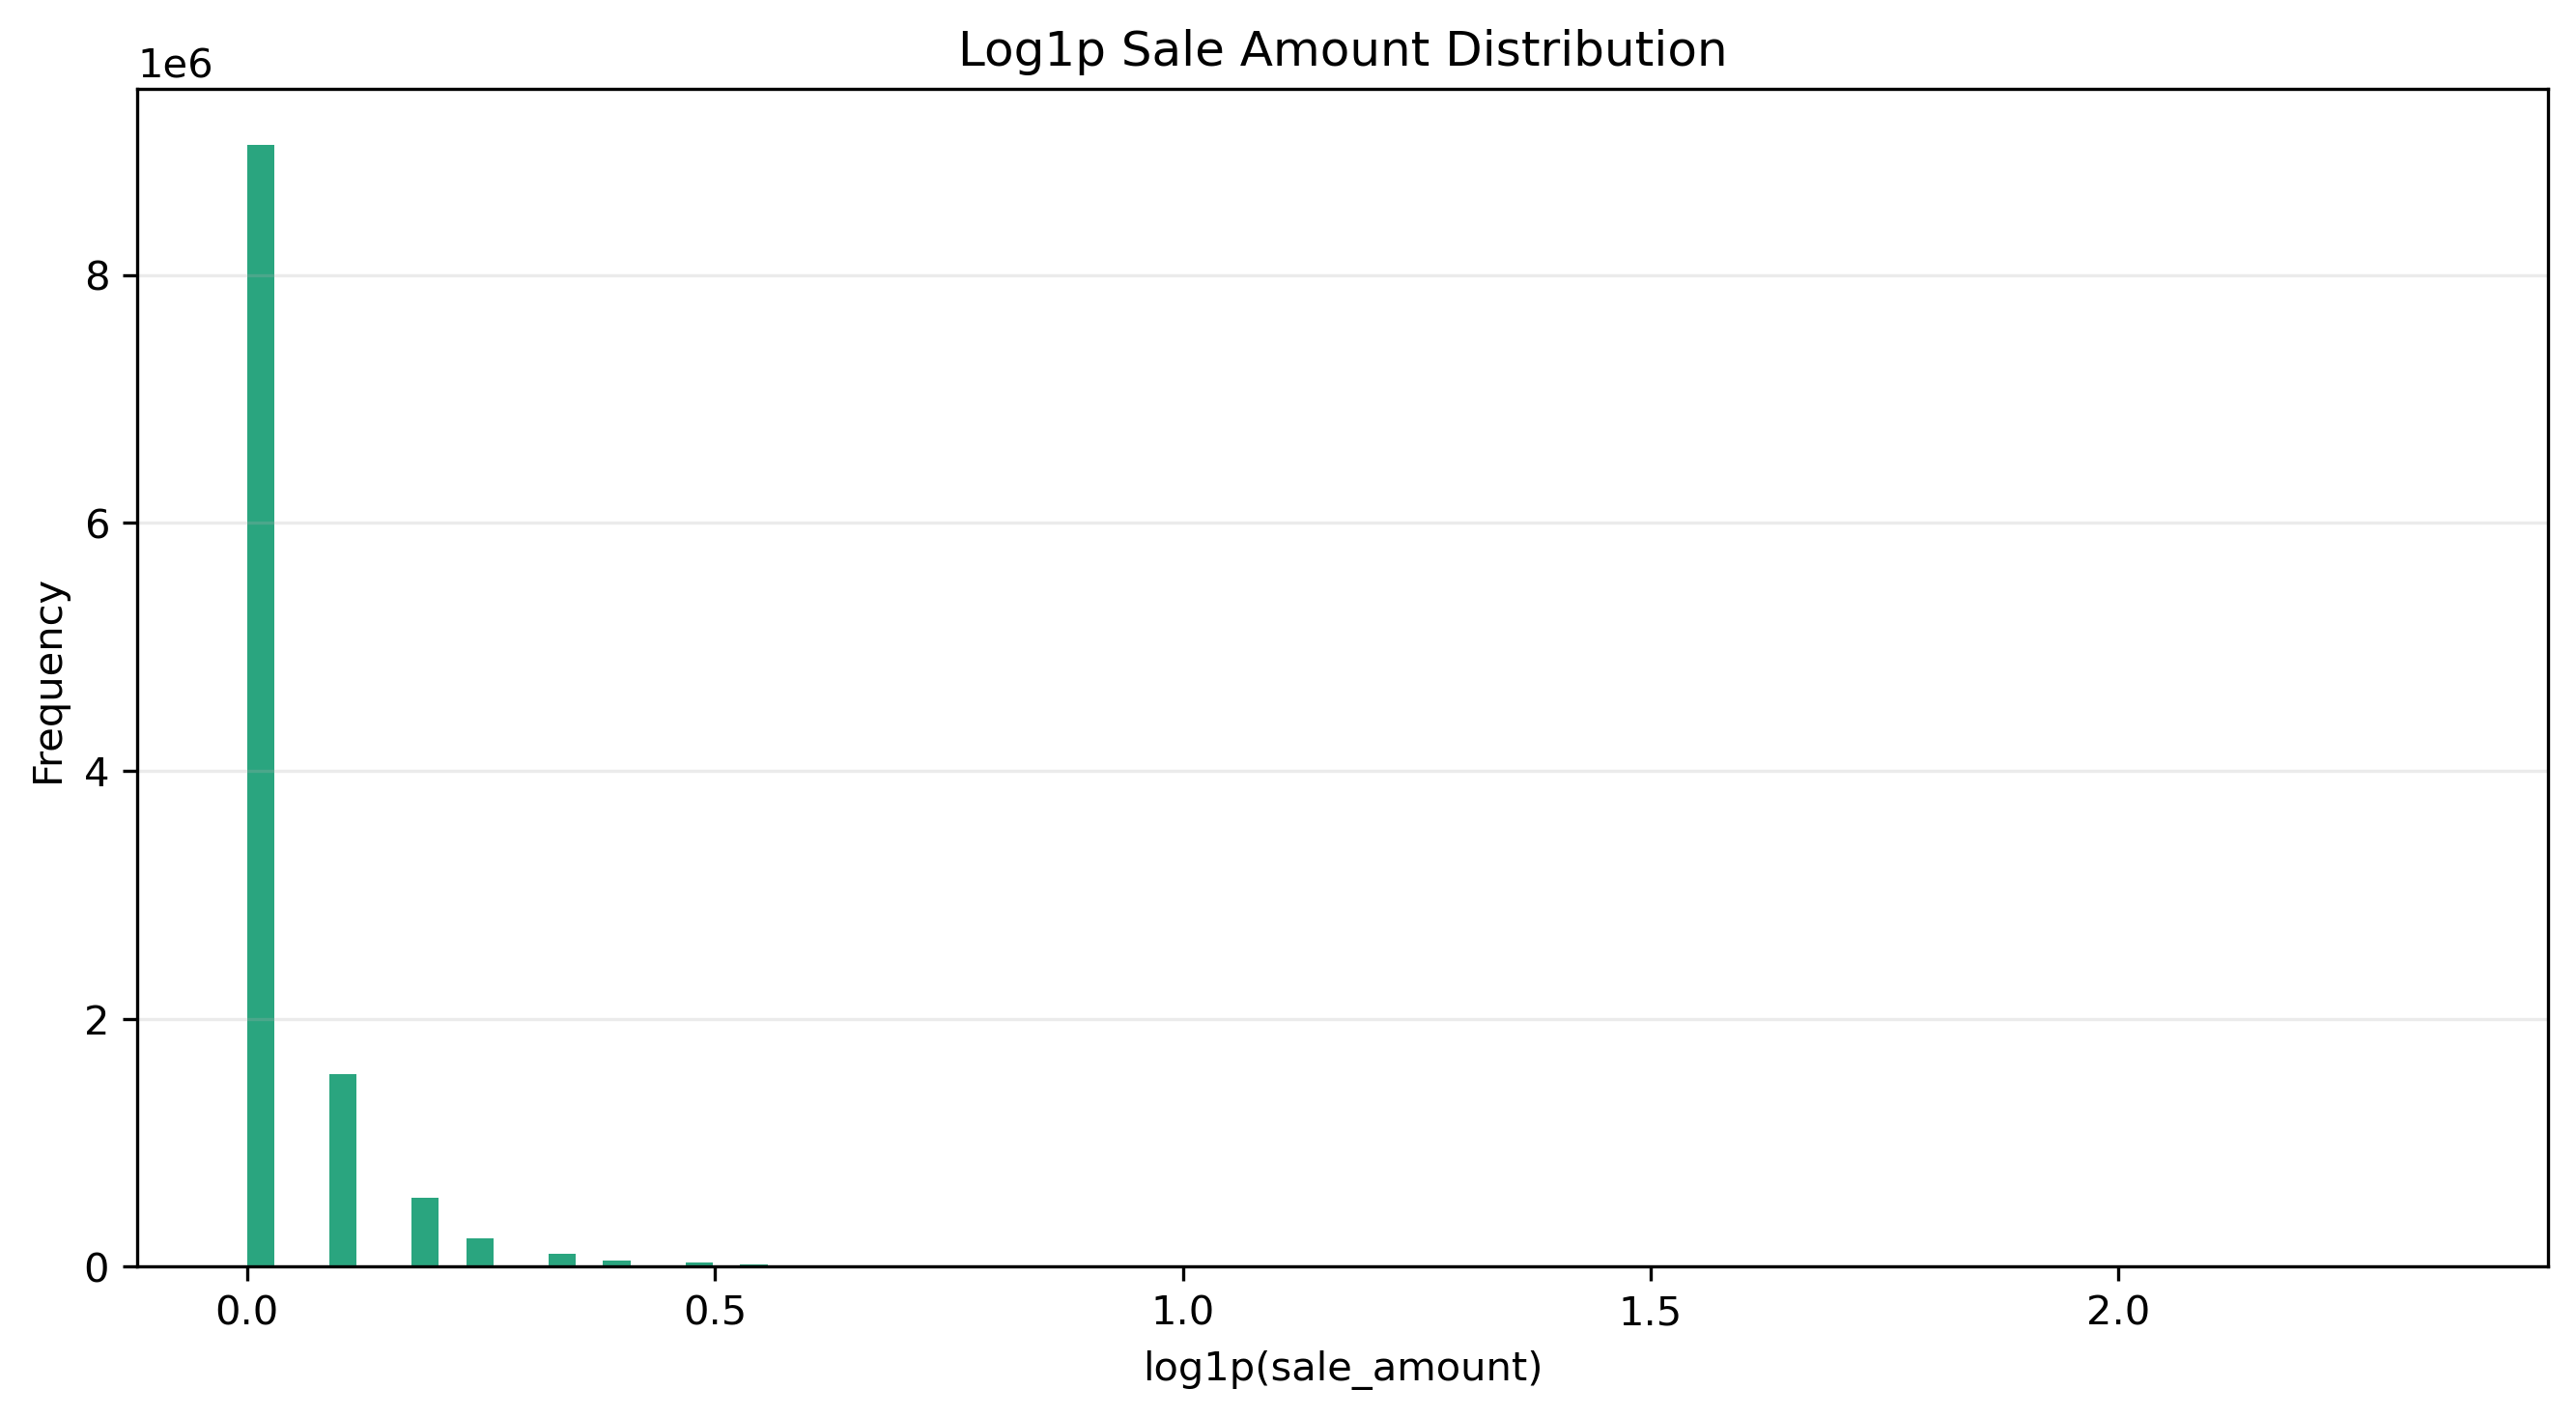
\includegraphics[width=0.78\linewidth]{figures/log_sale_amount_distribution.png}
    \caption{Phân phối log1p sale amount hourly.}
    \label{fig:long-log-sale-dist}
\end{figure}


\subsection{Seasonality theo giờ và theo tuần}

Seasonality là insight quan trọng nhất của dữ liệu. Sales thay đổi theo giờ trong ngày và theo thứ trong tuần. Điều này giải thích vì sao seasonal naive theo tuần là baseline rất mạnh ở phần kết quả. Trong bối cảnh bán lẻ, pattern tuần phản ánh hành vi mua sắm lặp lại của khách hàng, lịch hoạt động của cửa hàng và các chu kỳ khuyến mãi.


\begin{figure}[H]
    \centering
    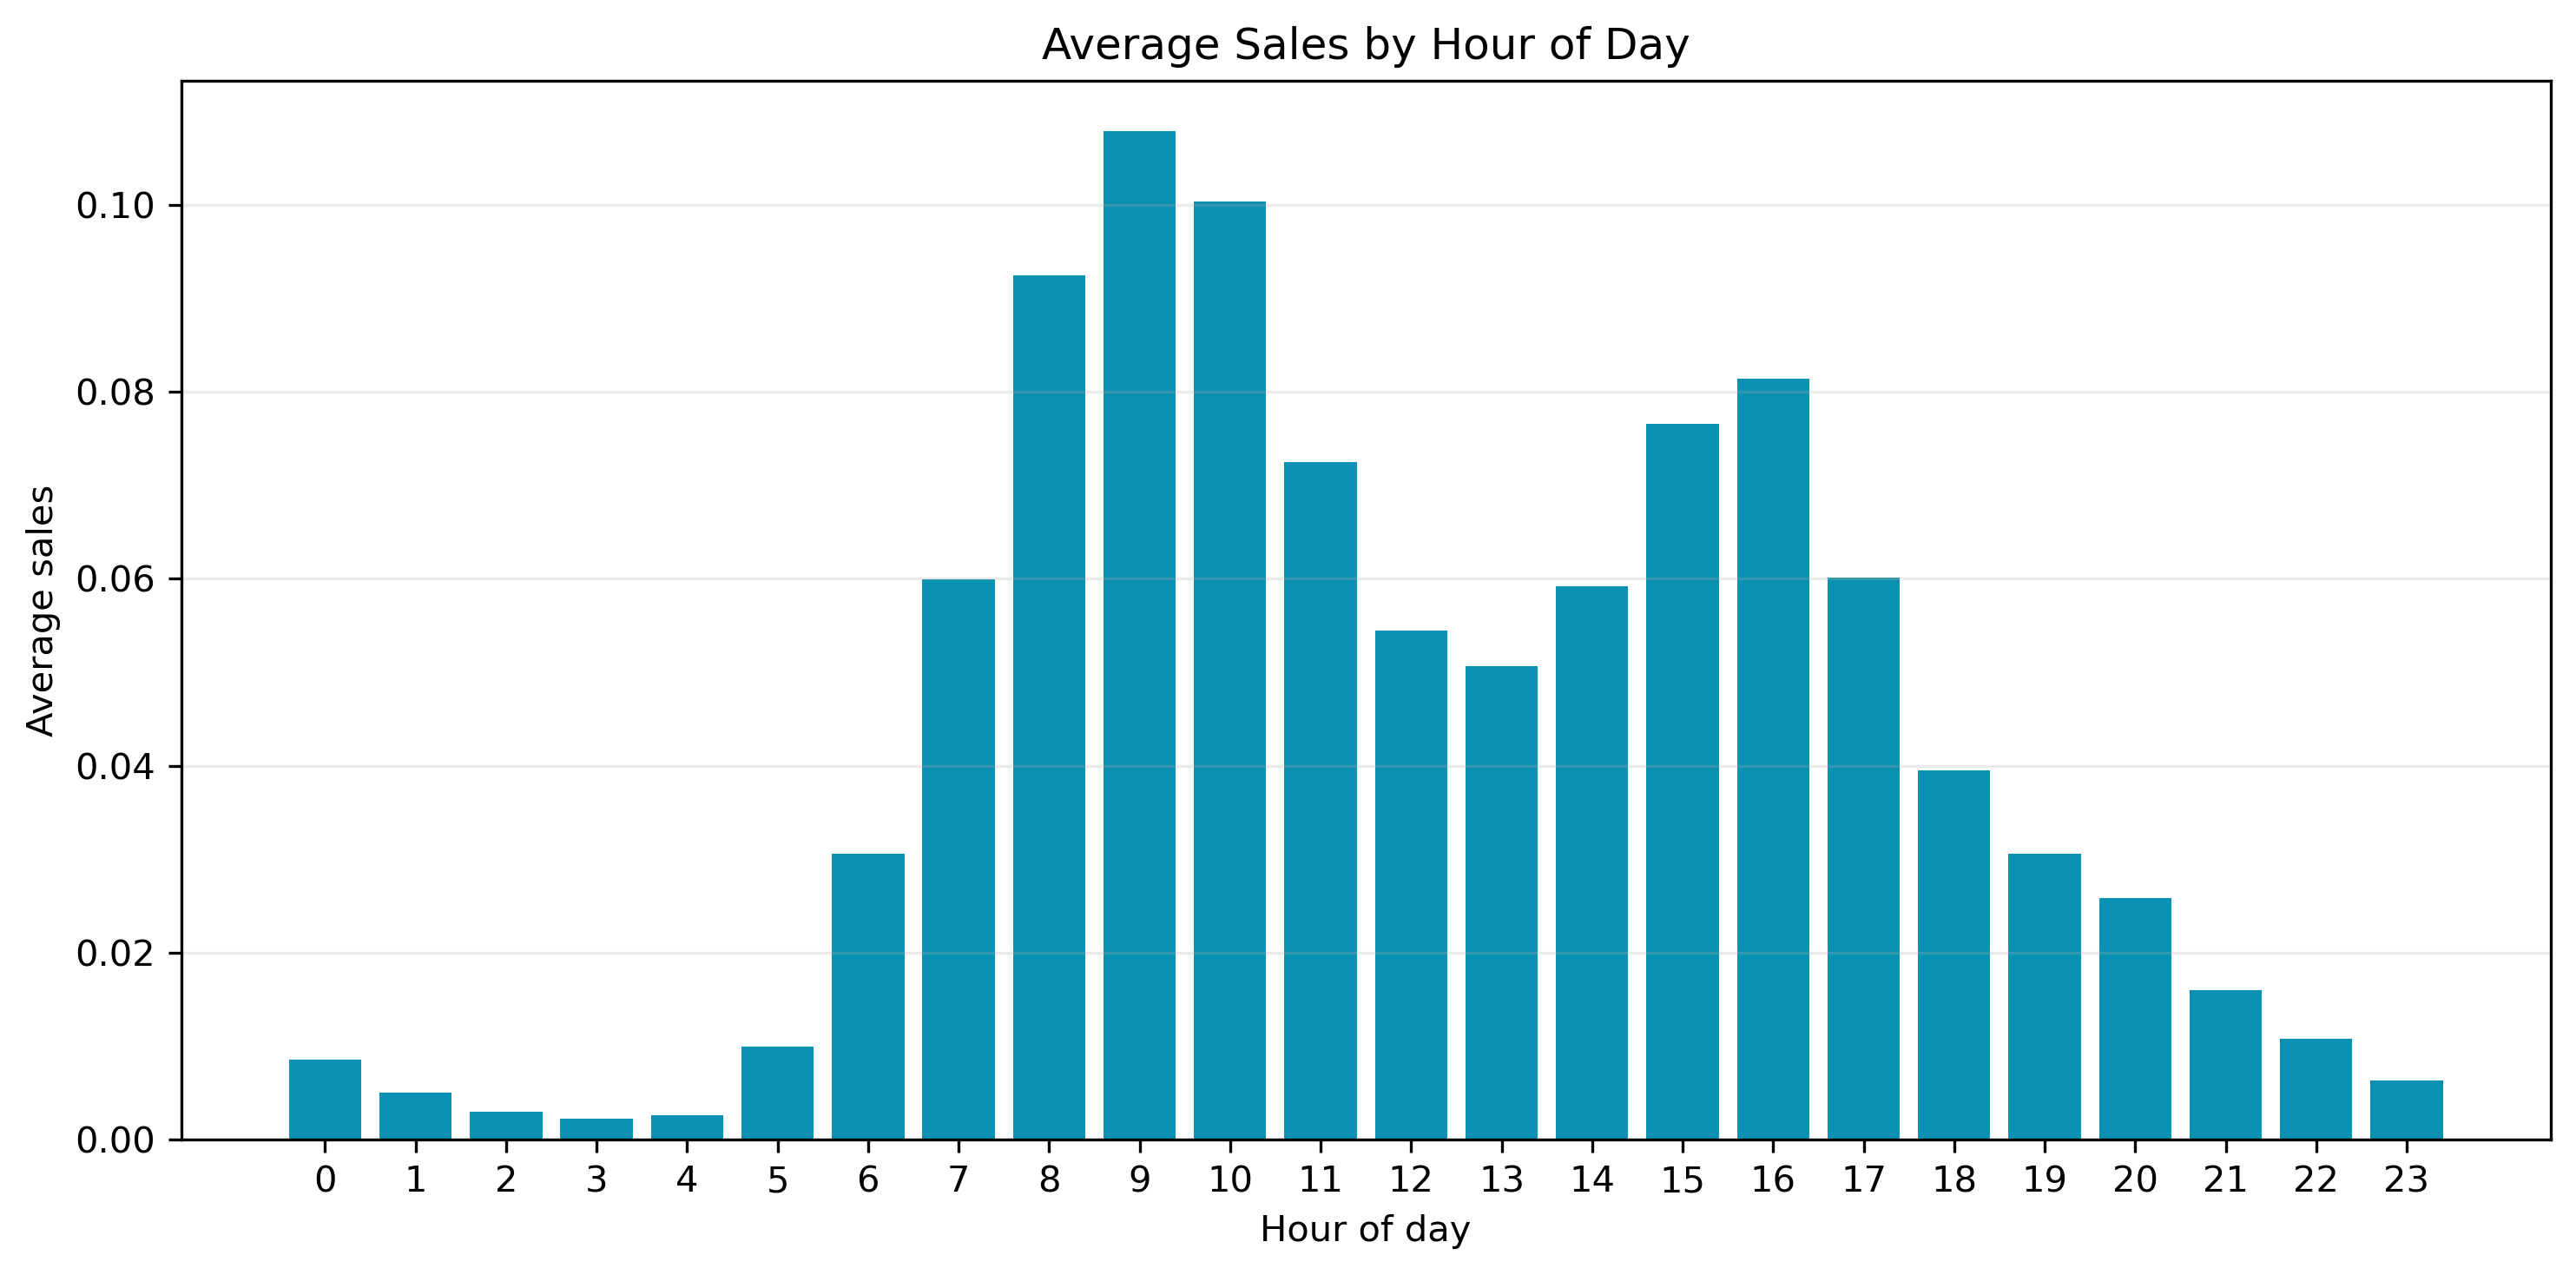
\includegraphics[width=0.78\linewidth]{figures/sales_by_hour_of_day.png}
    \caption{Sales trung bình theo giờ trong ngày.}
    \label{fig:long-hour-seasonality}
\end{figure}



\begin{figure}[H]
    \centering
    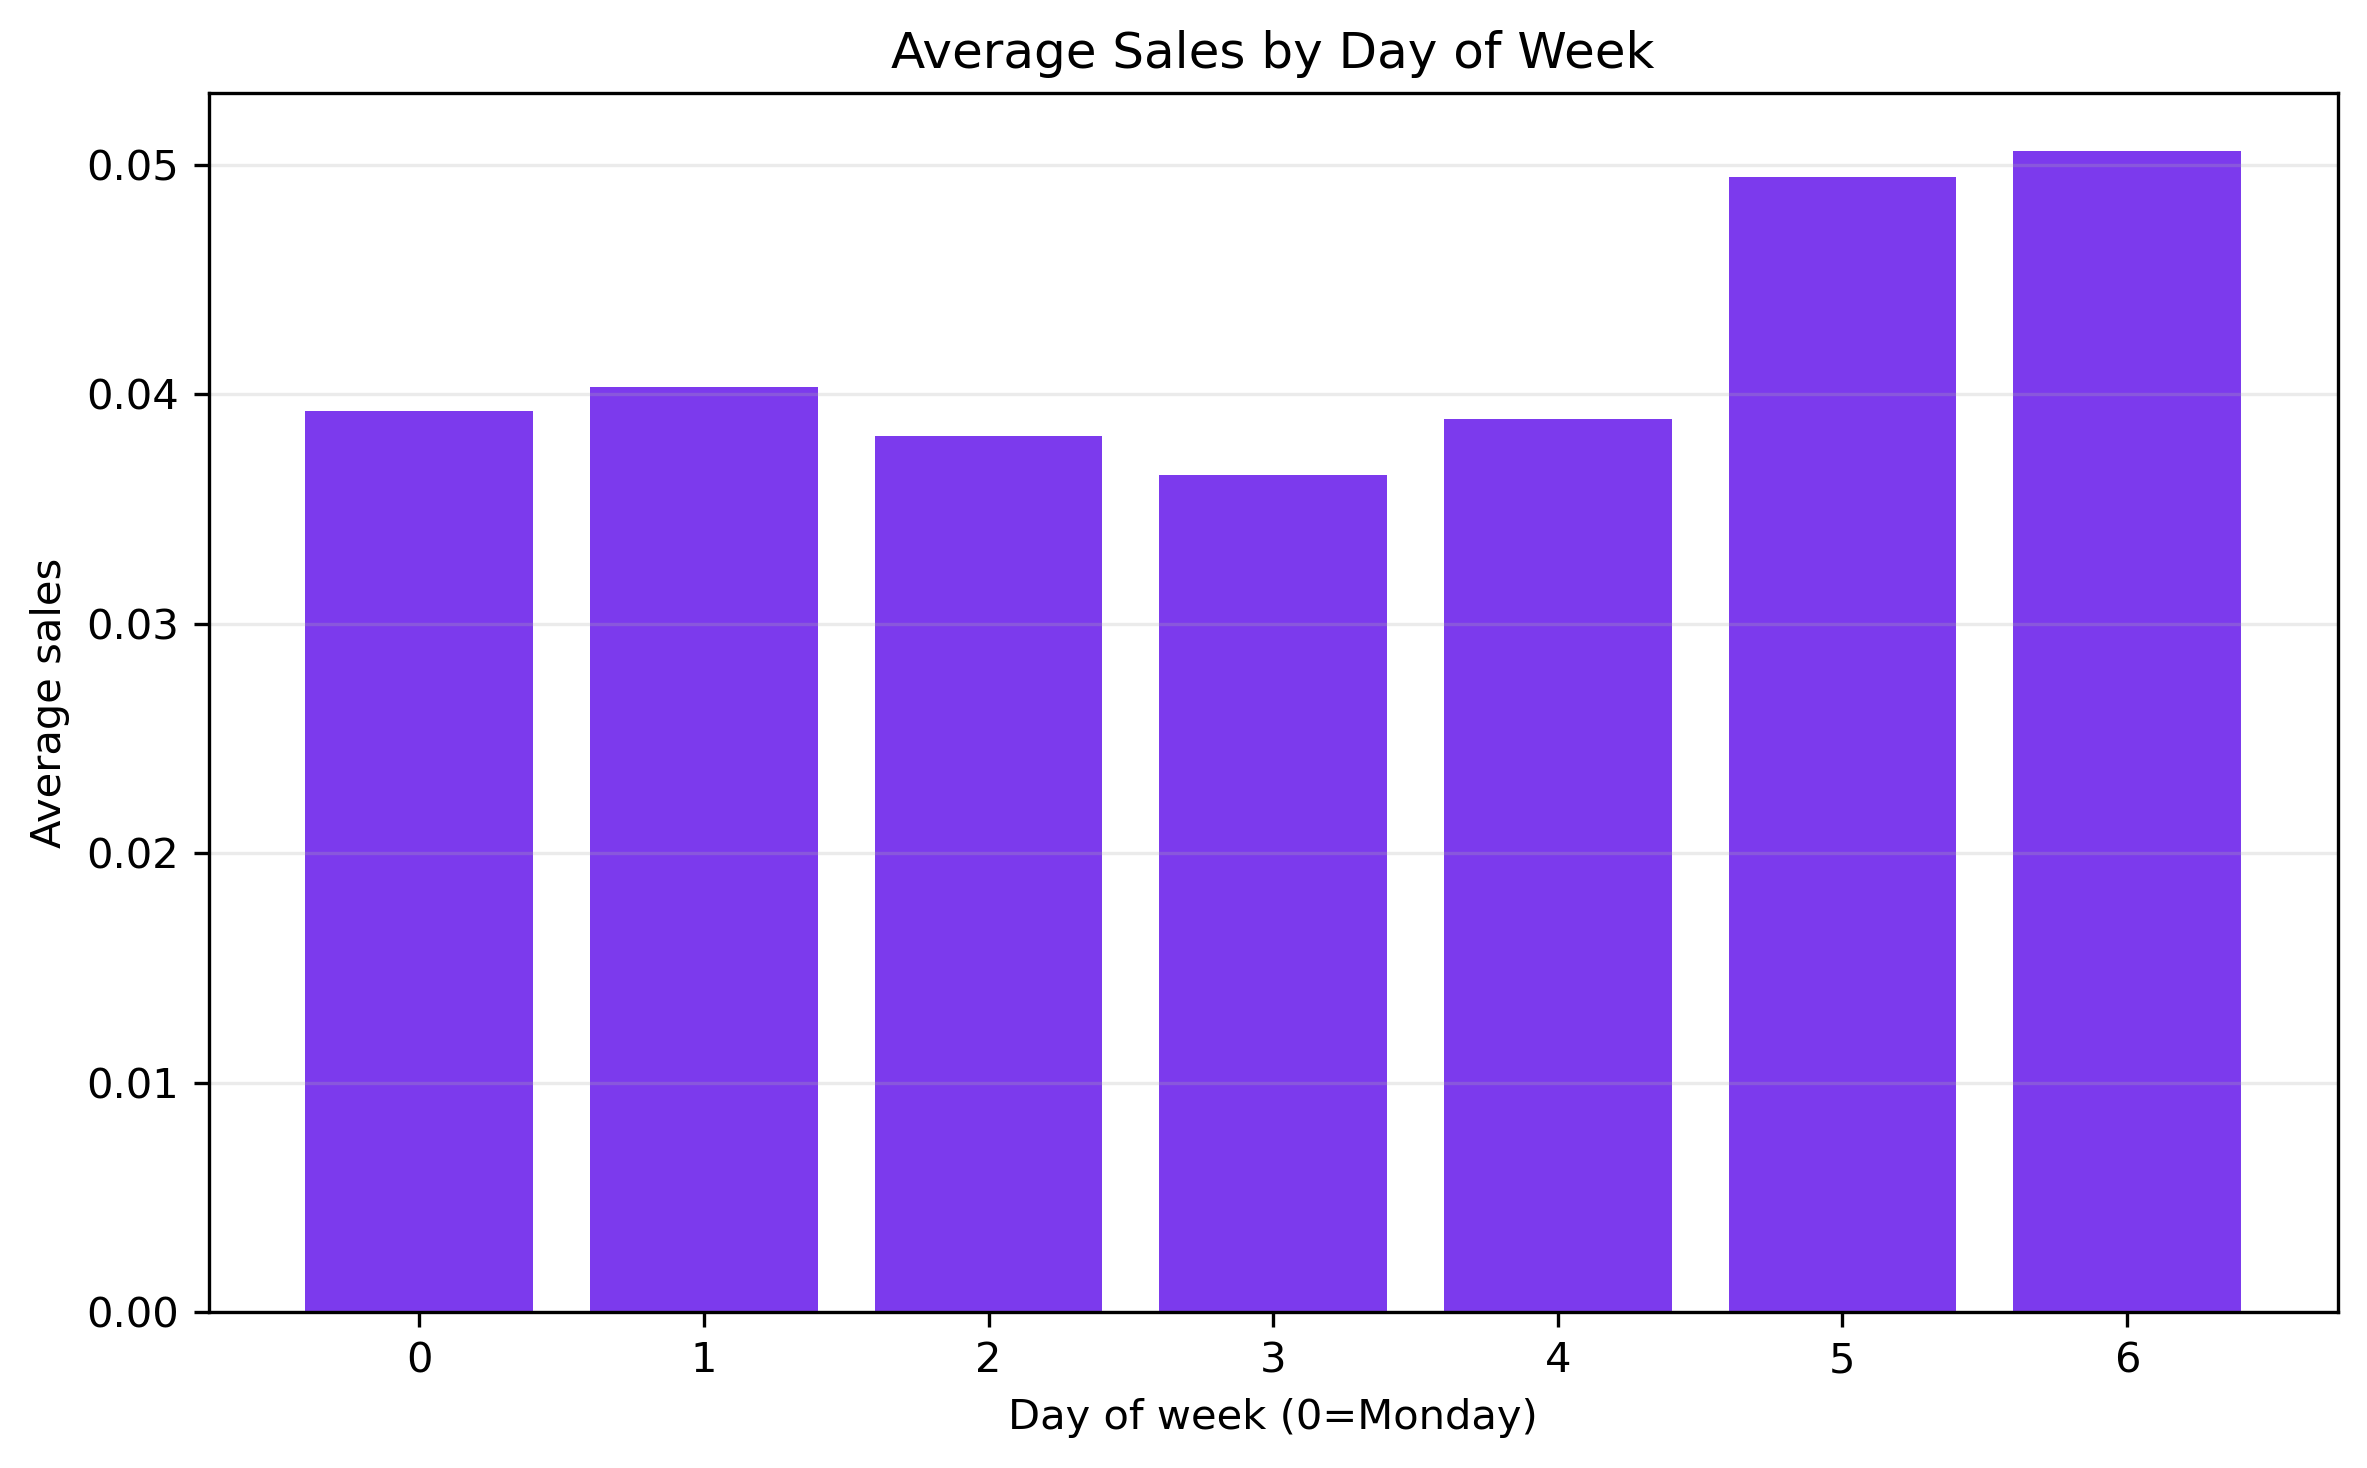
\includegraphics[width=0.78\linewidth]{figures/sales_by_day_of_week.png}
    \caption{Sales trung bình theo thứ trong tuần.}
    \label{fig:long-dow-seasonality}
\end{figure}


\subsection{Chuỗi đại diện}

Để không plot hàng nghìn chuỗi, báo cáo chọn ba chuỗi đại diện: high-volume, intermittent và stockout-heavy. Ba nhóm này minh họa ba kiểu khó khác nhau của forecasting: chuỗi lớn có pattern rõ, chuỗi thưa có nhiều zero, và chuỗi stockout-heavy có observed sales bị censor nặng.


\begin{table}[H]
\centering
\caption{Ba chuỗi đại diện}
\label{tab:long-representative}
\resizebox{0.86\linewidth}{!}{%
\begin{tabular}{lllll}
\toprule
series\_id & type & total\_sales & stockout\_rate & n\_obs \\
\midrule
4\_11\_267 & high\_volume & 1,896 & 0.6070 & 2328 \\
3\_793\_550 & intermittent & 49.7000 & 0.1907 & 2328 \\
5\_6\_757 & stockout\_heavy & 48.4000 & 0.7371 & 2328 \\
\bottomrule
\end{tabular}
}
\end{table}



\begin{figure}[H]
    \centering
    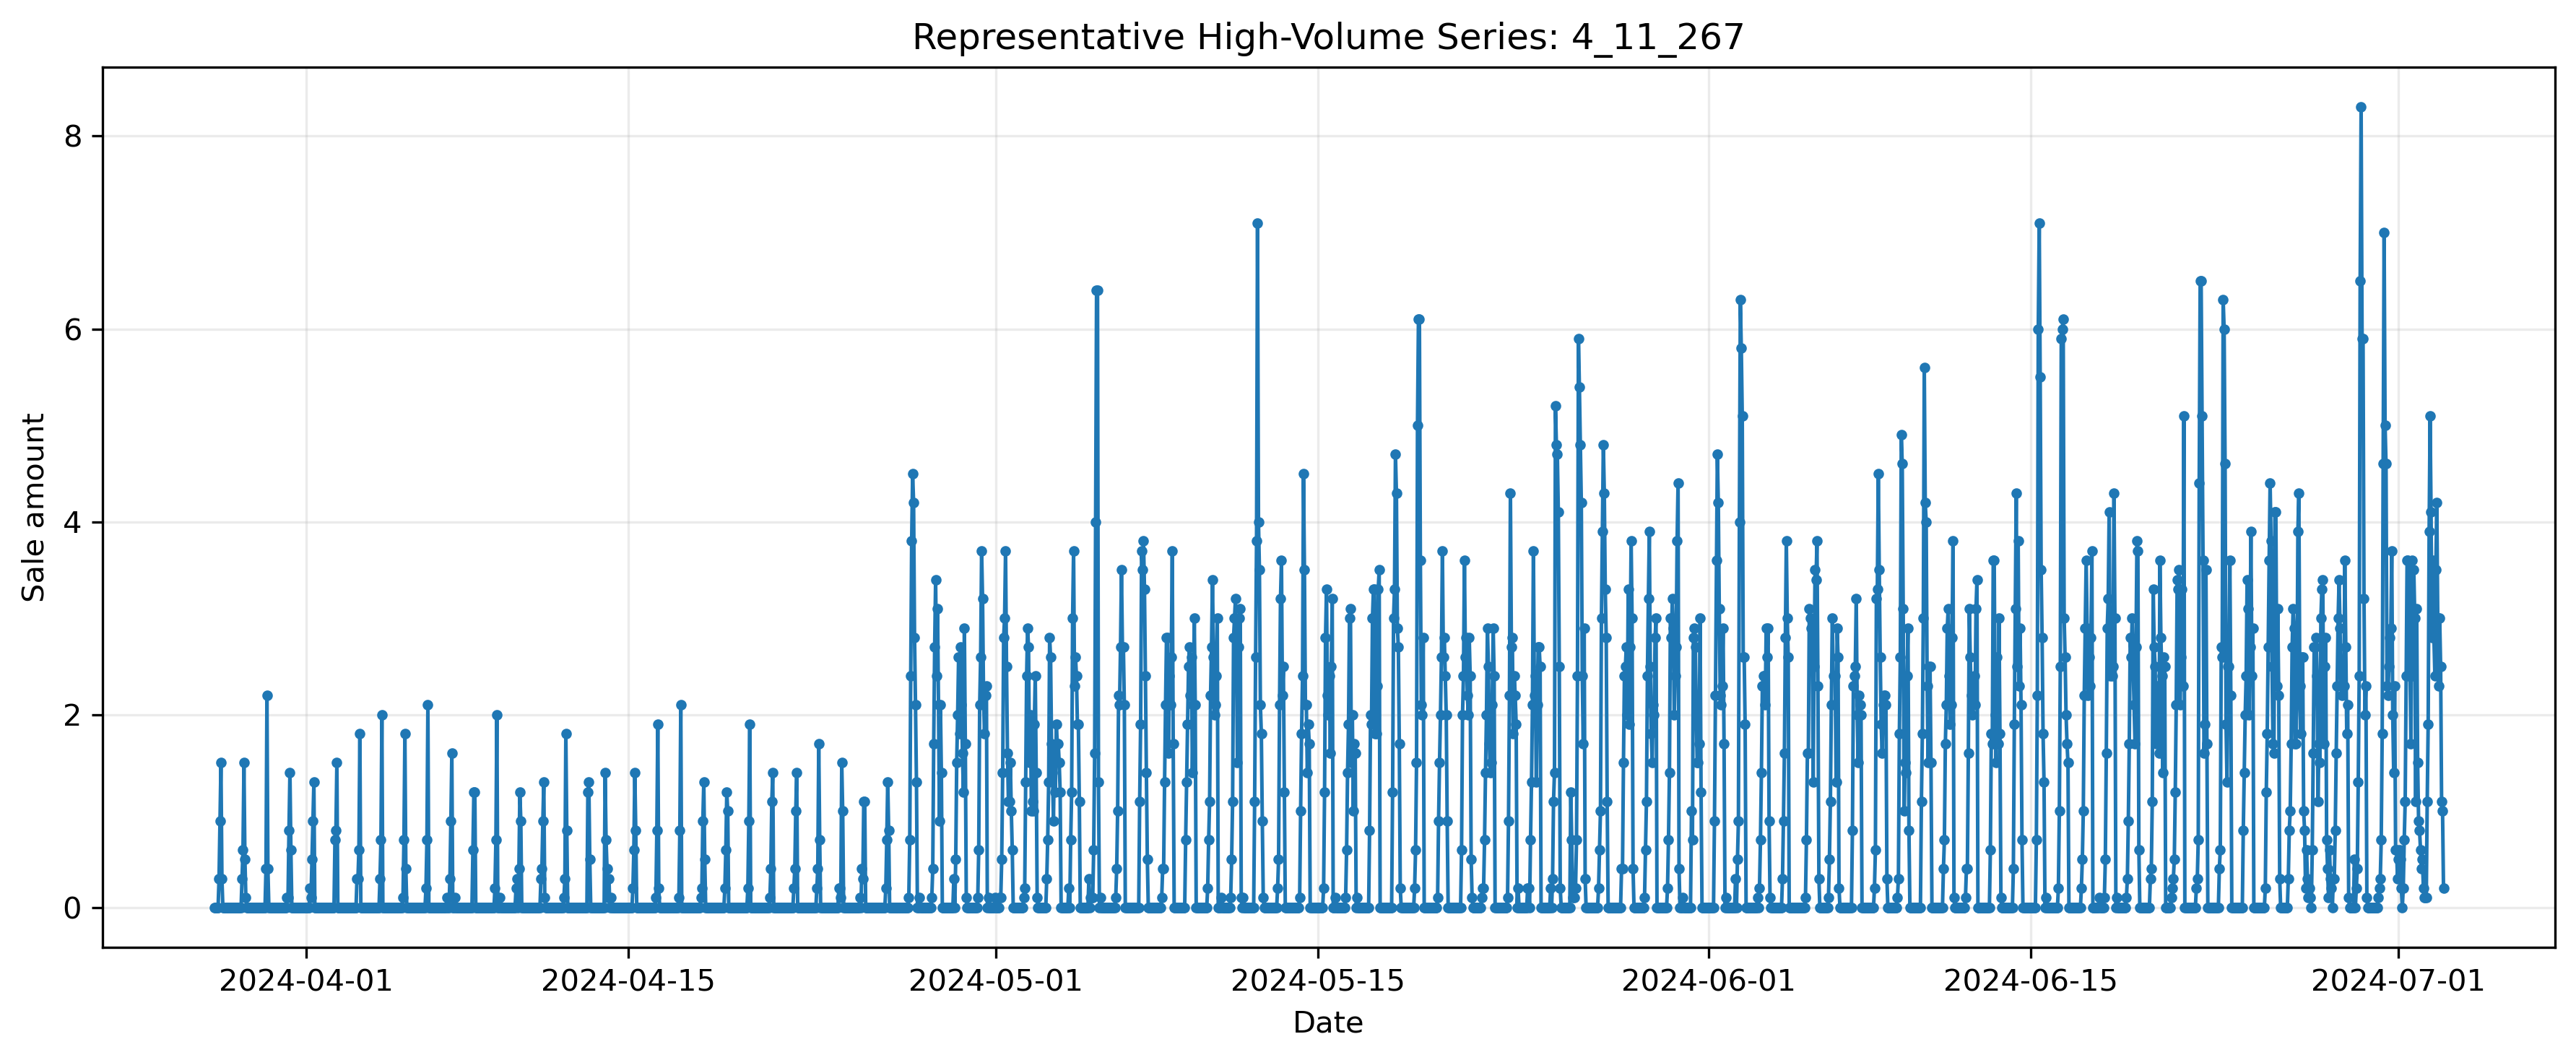
\includegraphics[width=0.92\linewidth]{figures/representative_series_high_volume.png}
    \caption{Chuỗi đại diện high-volume.}
    \label{fig:long-rep-high}
\end{figure}



\begin{figure}[H]
    \centering
    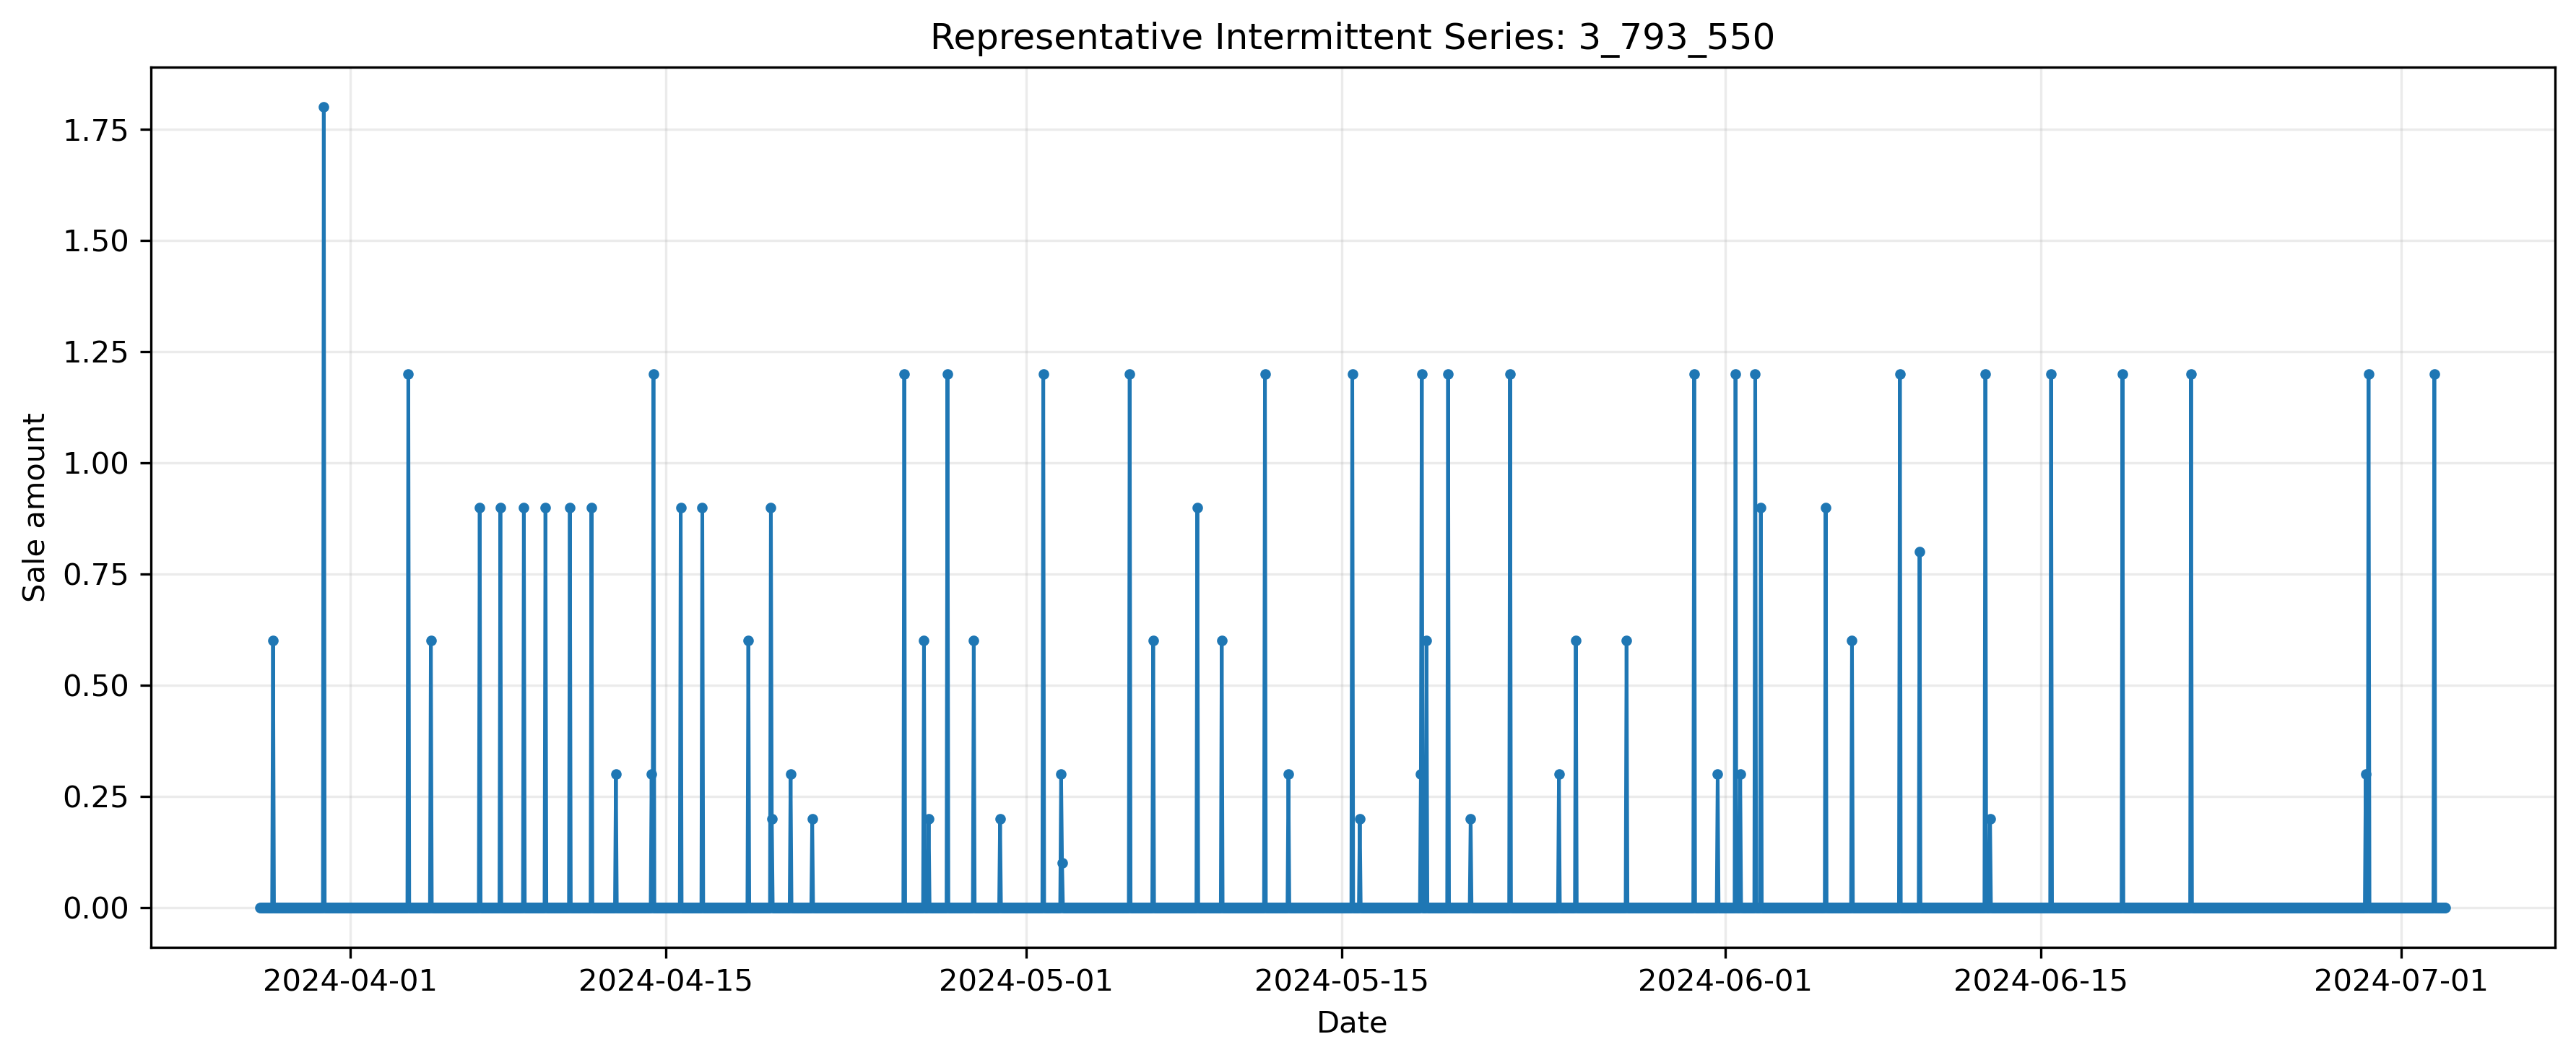
\includegraphics[width=0.92\linewidth]{figures/representative_series_intermittent.png}
    \caption{Chuỗi đại diện intermittent.}
    \label{fig:long-rep-intermittent}
\end{figure}



\begin{figure}[H]
    \centering
    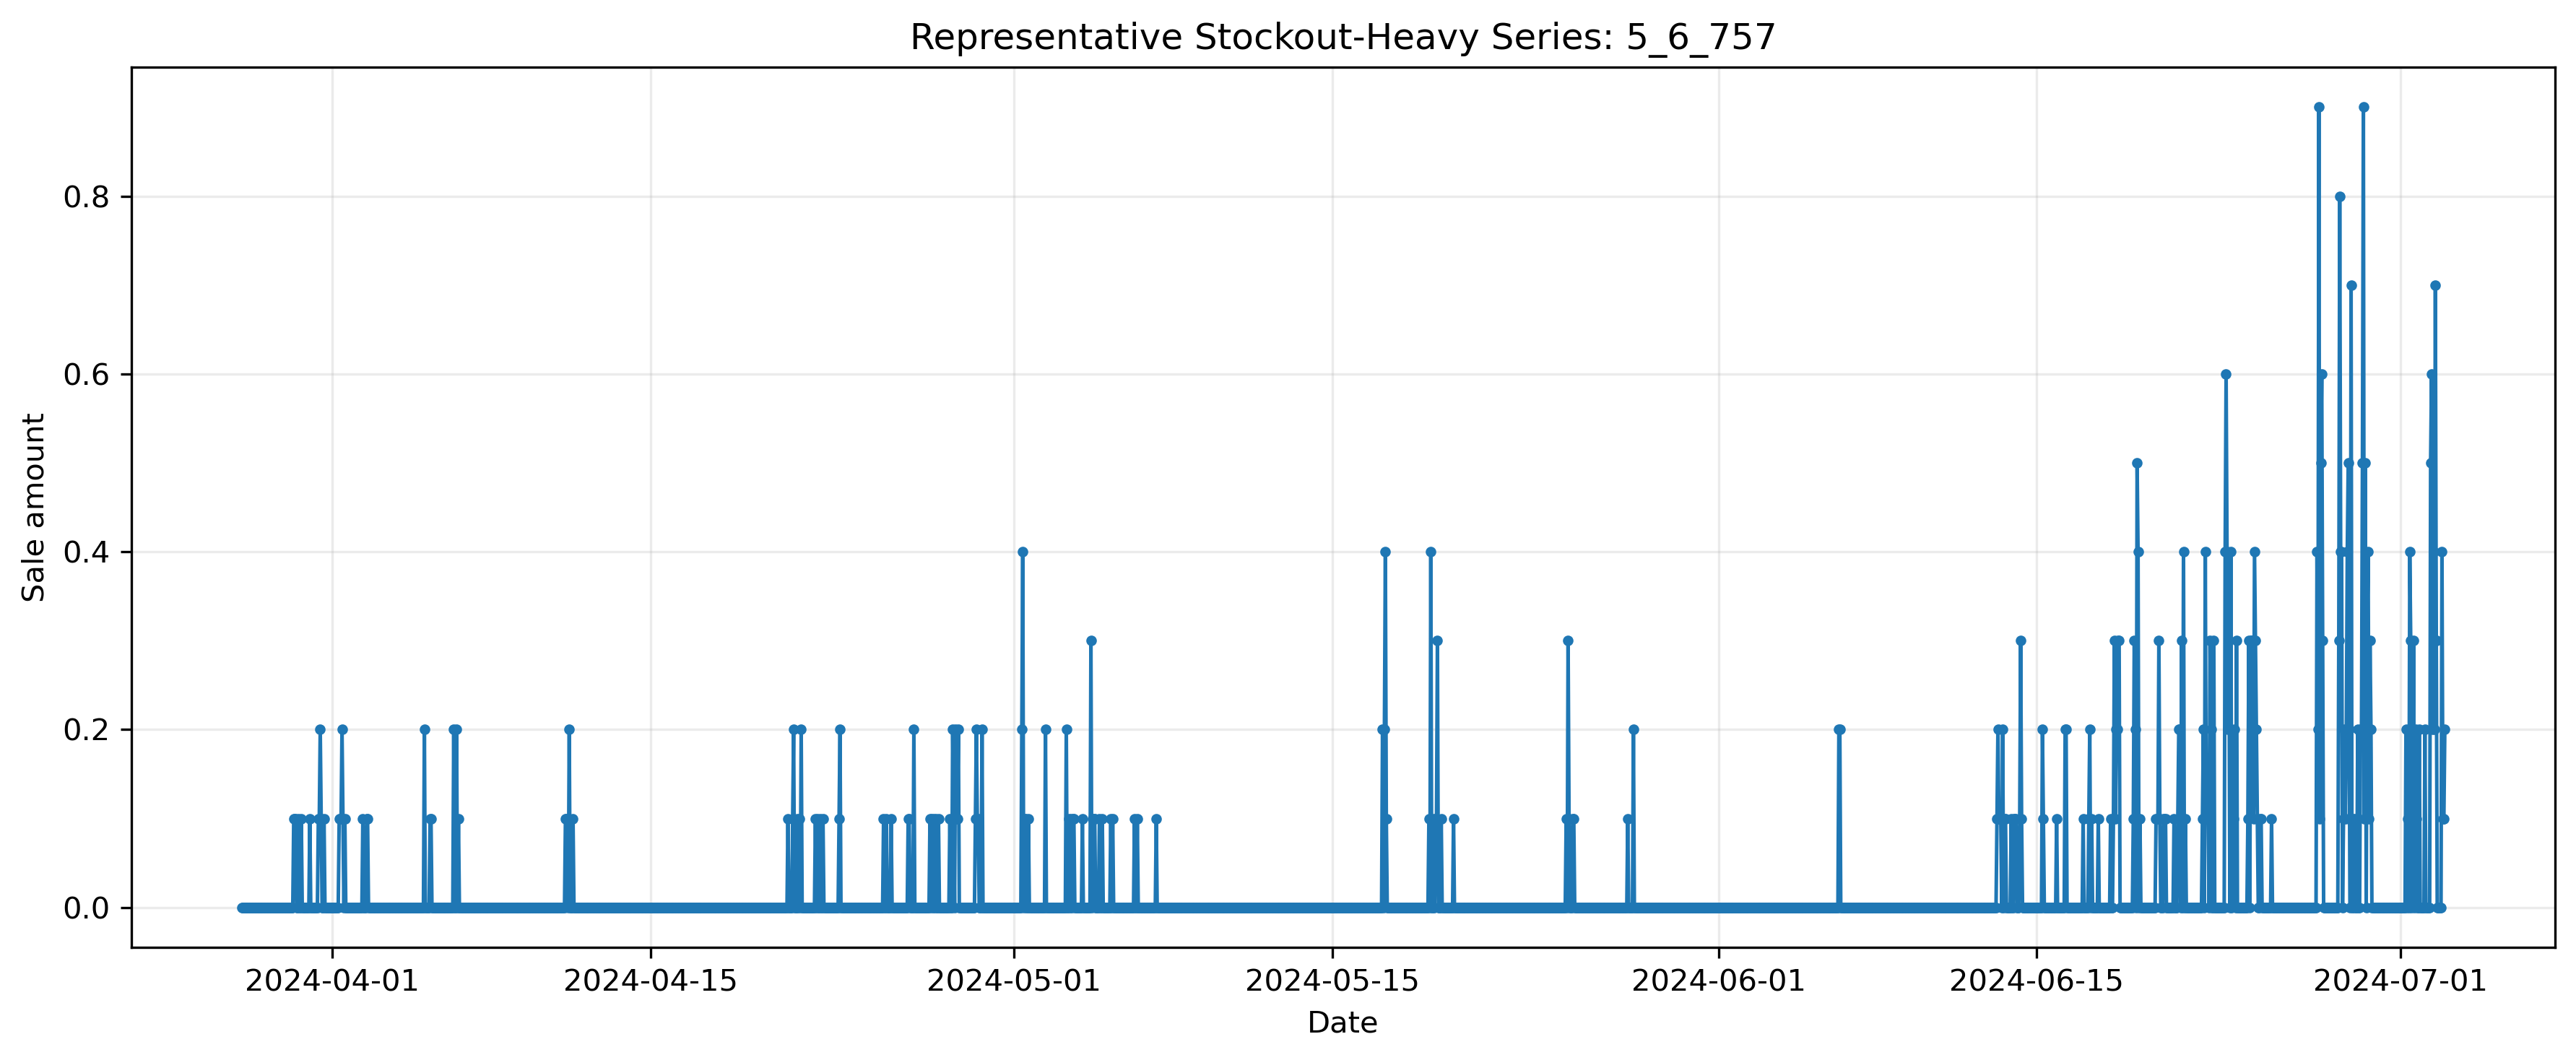
\includegraphics[width=0.92\linewidth]{figures/representative_series_stockout_heavy.png}
    \caption{Chuỗi đại diện stockout-heavy.}
    \label{fig:long-rep-stockout}
\end{figure}

\section{Kiểm tra time-series: stationarity, ACF/PACF và spectrum}

\subsection{Stationarity testing}

Theo yêu cầu môn học, báo cáo vẫn thực hiện ADF và KPSS trên aggregate series và các chuỗi đại diện. Tuy nhiên, với bài toán nhiều chuỗi bán lẻ, mục đích của stationarity test không phải để ép toàn bộ pipeline thành ARIMA cổ điển. Thay vào đó, ADF/KPSS giúp nhận diện mức độ trend/seasonality và củng cố quyết định dùng lag, rolling và seasonal baseline.


\begin{table}[H]
\centering
\caption{Kết quả ADF/KPSS}
\label{tab:long-stationarity}
\resizebox{\linewidth}{!}{%
\begin{tabular}{llllll}
\toprule
Series & Transformation & ADF p-value & KPSS p-value & Conclusion & N \\
\midrule
aggregate\_hourly\_sales & original & 0.0000 & 0.0100 & mixed evidence & 2328 \\
aggregate\_hourly\_sales & log1p & 0.0000 & 0.0100 & mixed evidence & 2328 \\
aggregate\_hourly\_sales & first\_difference & 0.0000 & 0.1000 & stationary & 2327 \\
aggregate\_hourly\_sales & seasonal\_difference\_lag\_24 & 0.0000 & 0.1000 & stationary & 2304 \\
high\_volume\_series & original & 0.3070 & 0.0100 & non-stationary & 2328 \\
high\_volume\_series & log1p & 0.4265 & 0.0100 & non-stationary & 2328 \\
high\_volume\_series & first\_difference & 0.0000 & 0.1000 & stationary & 2327 \\
high\_volume\_series & seasonal\_difference\_lag\_24 & 0.0000 & 0.1000 & stationary & 2304 \\
intermittent\_series & original & 0.0000 & 0.1000 & stationary & 2328 \\
intermittent\_series & log1p & 0.0000 & 0.1000 & stationary & 2328 \\
intermittent\_series & first\_difference & 0.0000 & 0.1000 & stationary & 2327 \\
intermittent\_series & seasonal\_difference\_lag\_24 & 0.0000 & 0.1000 & stationary & 2304 \\
stockout\_heavy\_series & original & 0.0058 & 0.0100 & mixed evidence & 2328 \\
stockout\_heavy\_series & log1p & 0.0031 & 0.0100 & mixed evidence & 2328 \\
stockout\_heavy\_series & first\_difference & 0.0000 & 0.1000 & stationary & 2327 \\
stockout\_heavy\_series & seasonal\_difference\_lag\_24 & 0.0000 & 0.1000 & stationary & 2304 \\
\bottomrule
\end{tabular}
}
\end{table}


\subsection{ACF/PACF}

ACF/PACF cho thấy autocorrelation và seasonal dependence ở các lag ngắn và lag theo ngày/tuần. Với dữ liệu hourly, lag 24 và 168 có ý nghĩa tự nhiên. Trong pipeline cuối, recovery được làm ở cấp hourly, còn forecasting được aggregate lên daily và dùng lag 7/14/28 ngày.


\begin{figure}[H]
    \centering
    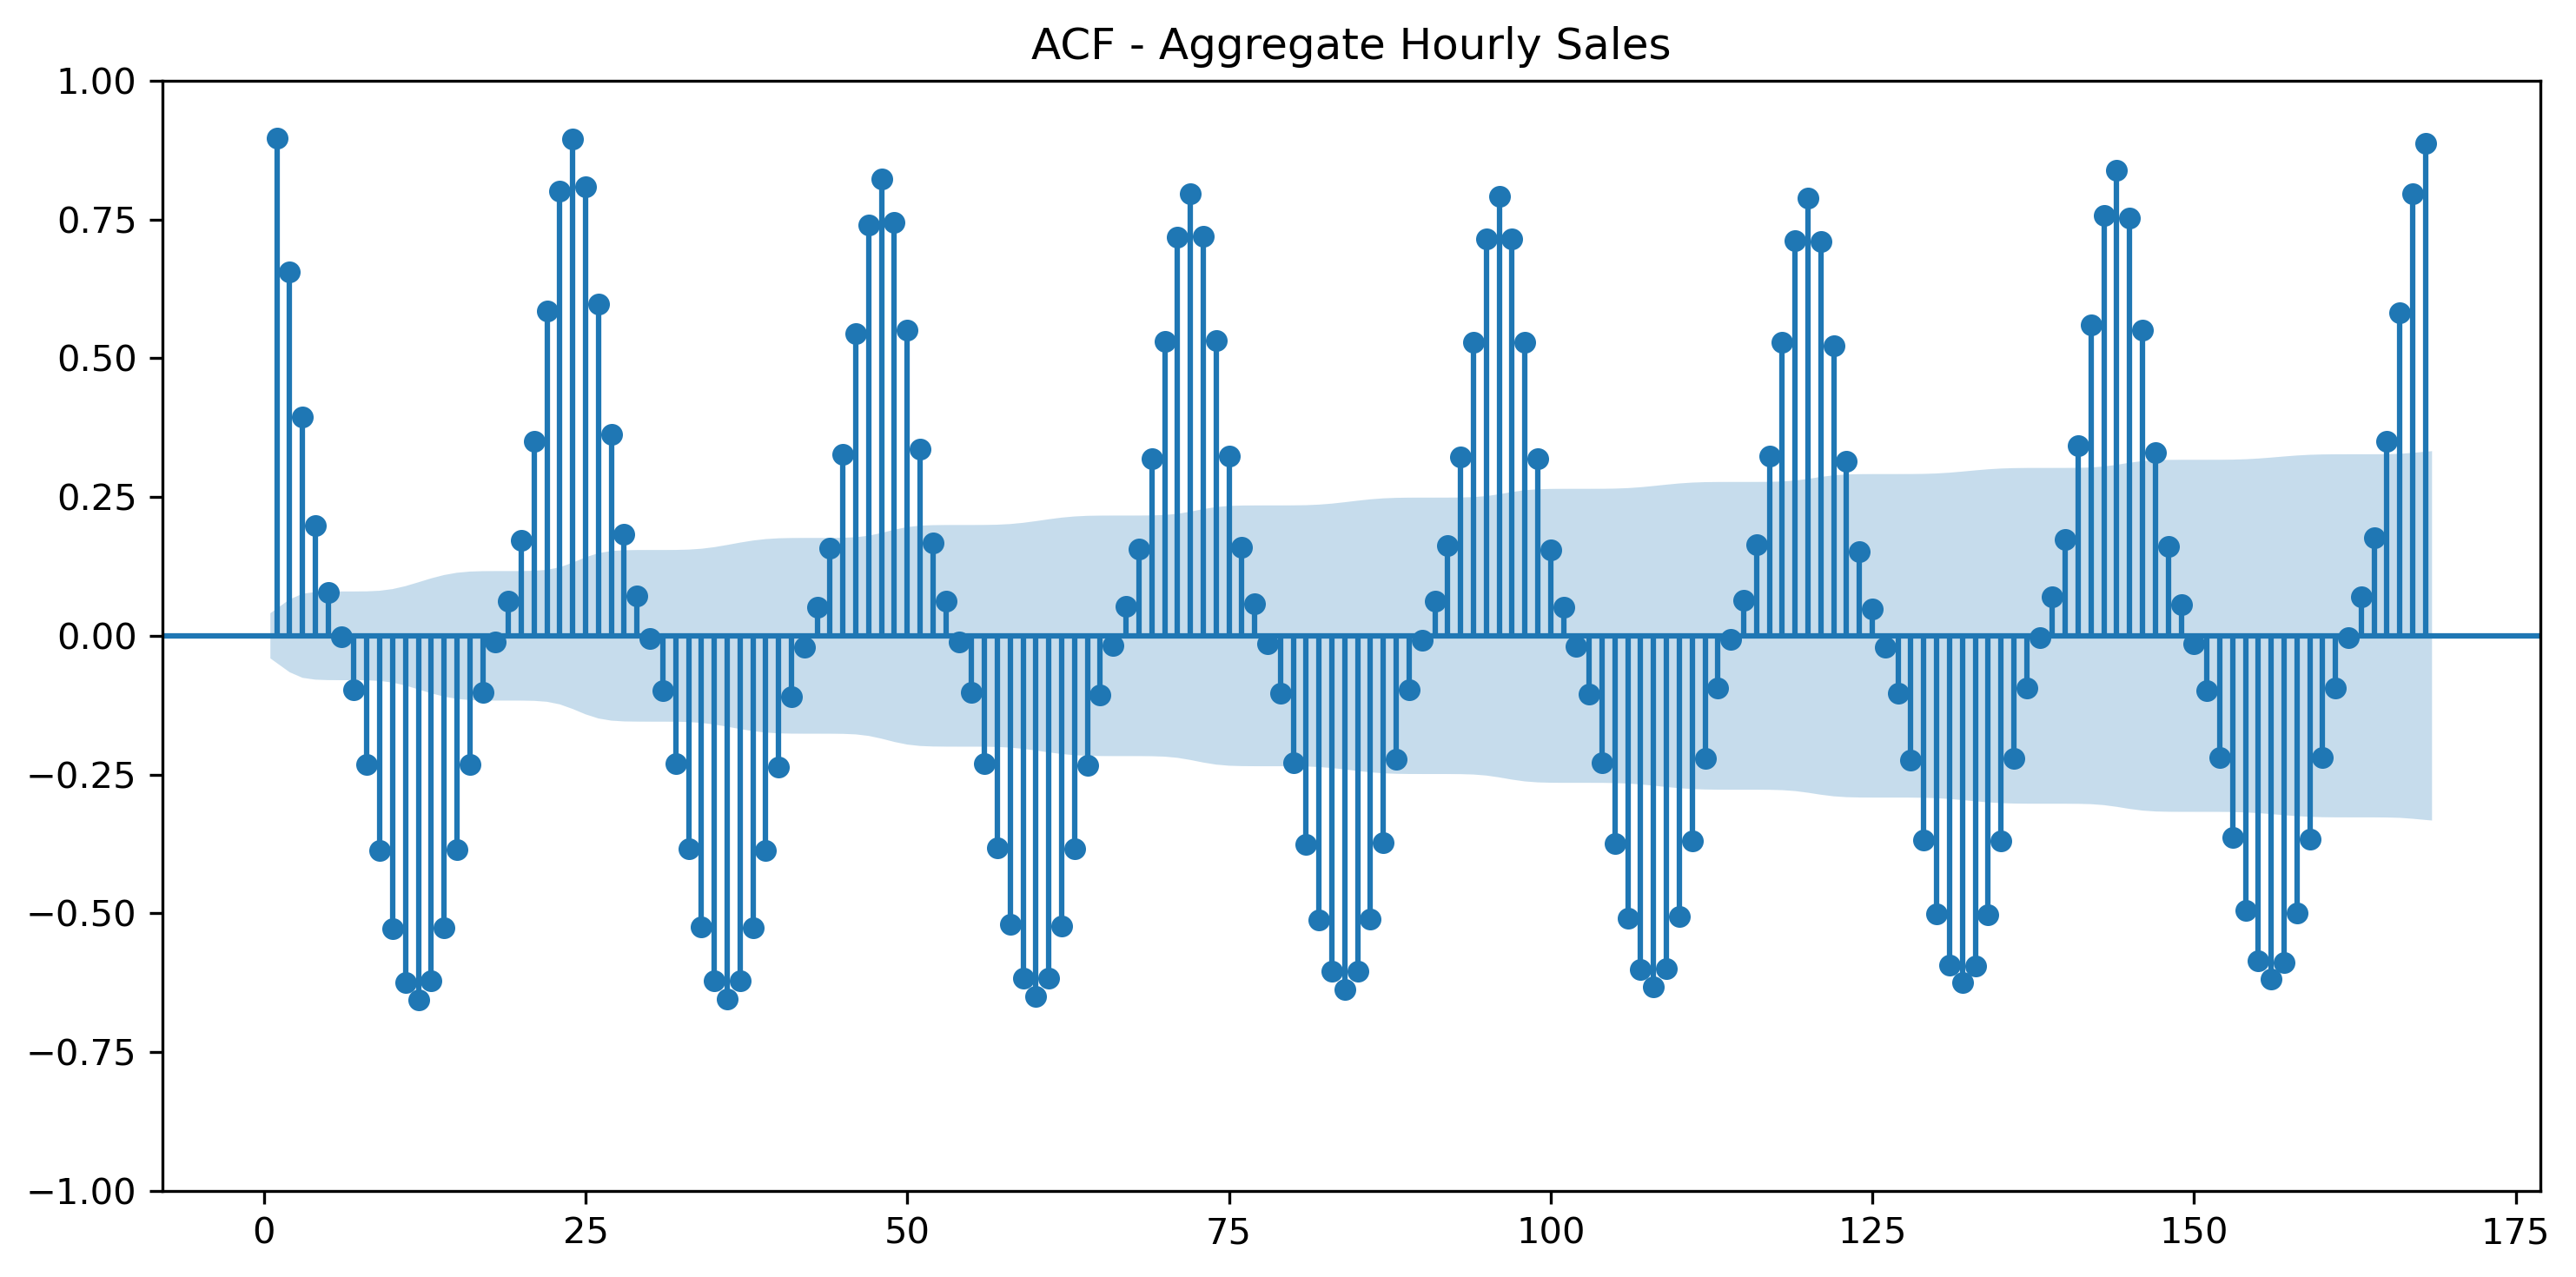
\includegraphics[width=0.84\linewidth]{figures/acf_aggregate_sales.png}
    \caption{ACF của aggregate hourly sales.}
    \label{fig:long-acf-agg}
\end{figure}



\begin{figure}[H]
    \centering
    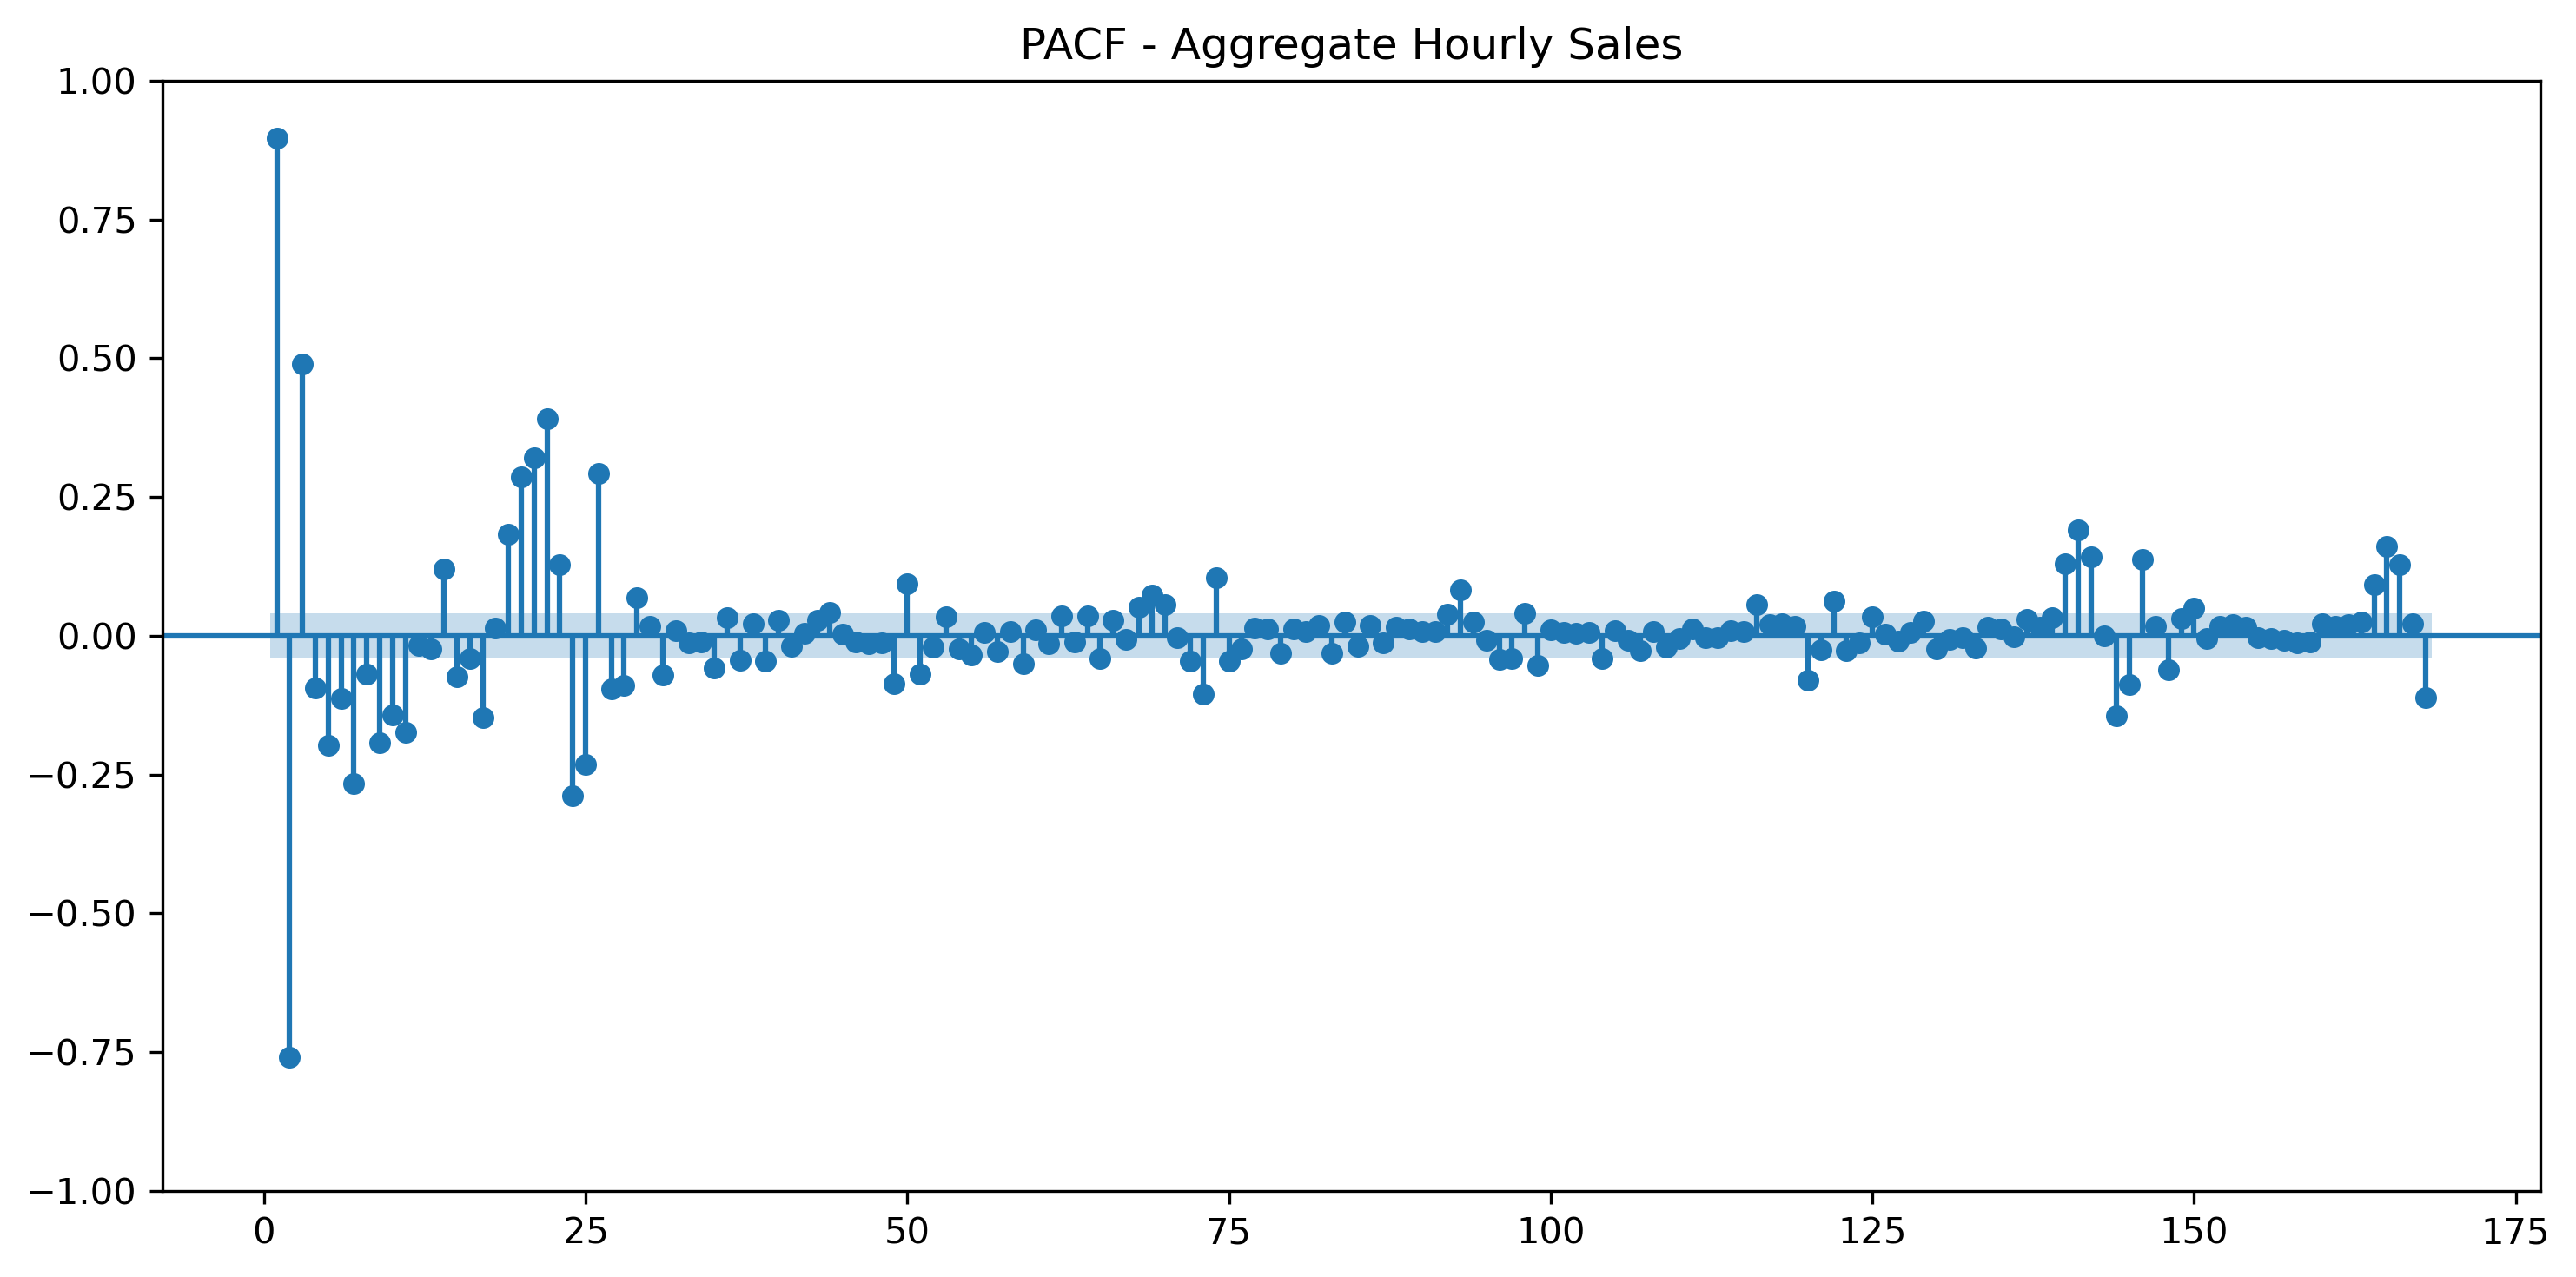
\includegraphics[width=0.84\linewidth]{figures/pacf_aggregate_sales.png}
    \caption{PACF của aggregate hourly sales.}
    \label{fig:long-pacf-agg}
\end{figure}



\begin{figure}[H]
    \centering
    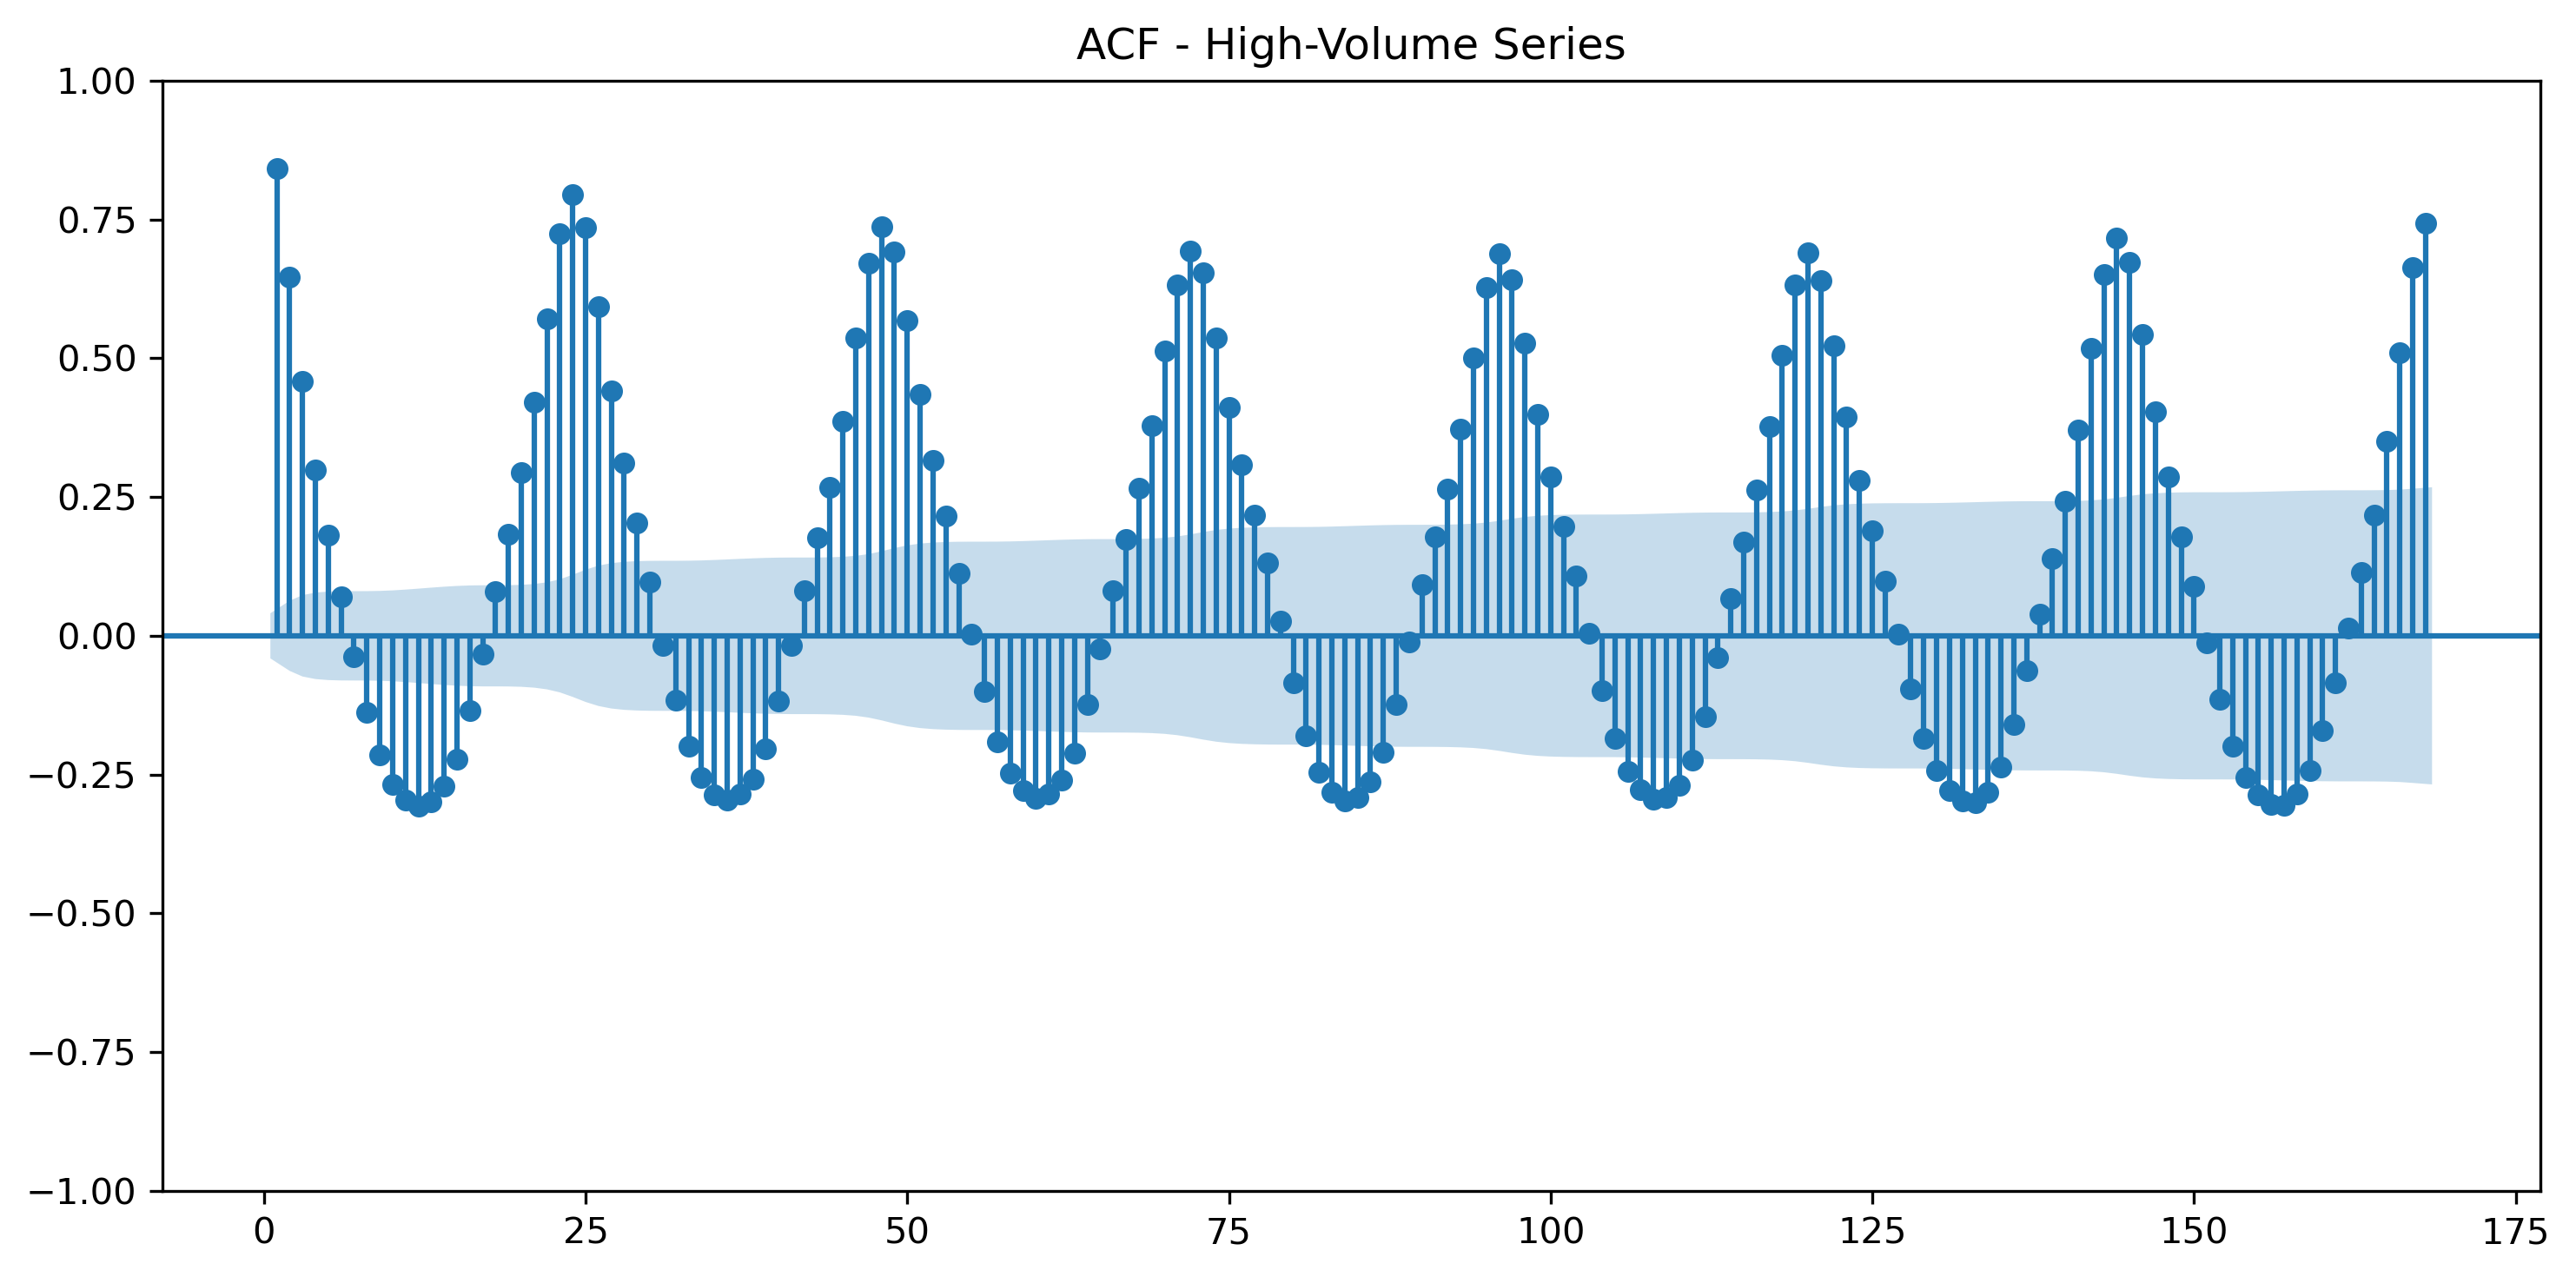
\includegraphics[width=0.84\linewidth]{figures/acf_high_volume_series.png}
    \caption{ACF của chuỗi high-volume.}
    \label{fig:long-acf-high}
\end{figure}



\begin{figure}[H]
    \centering
    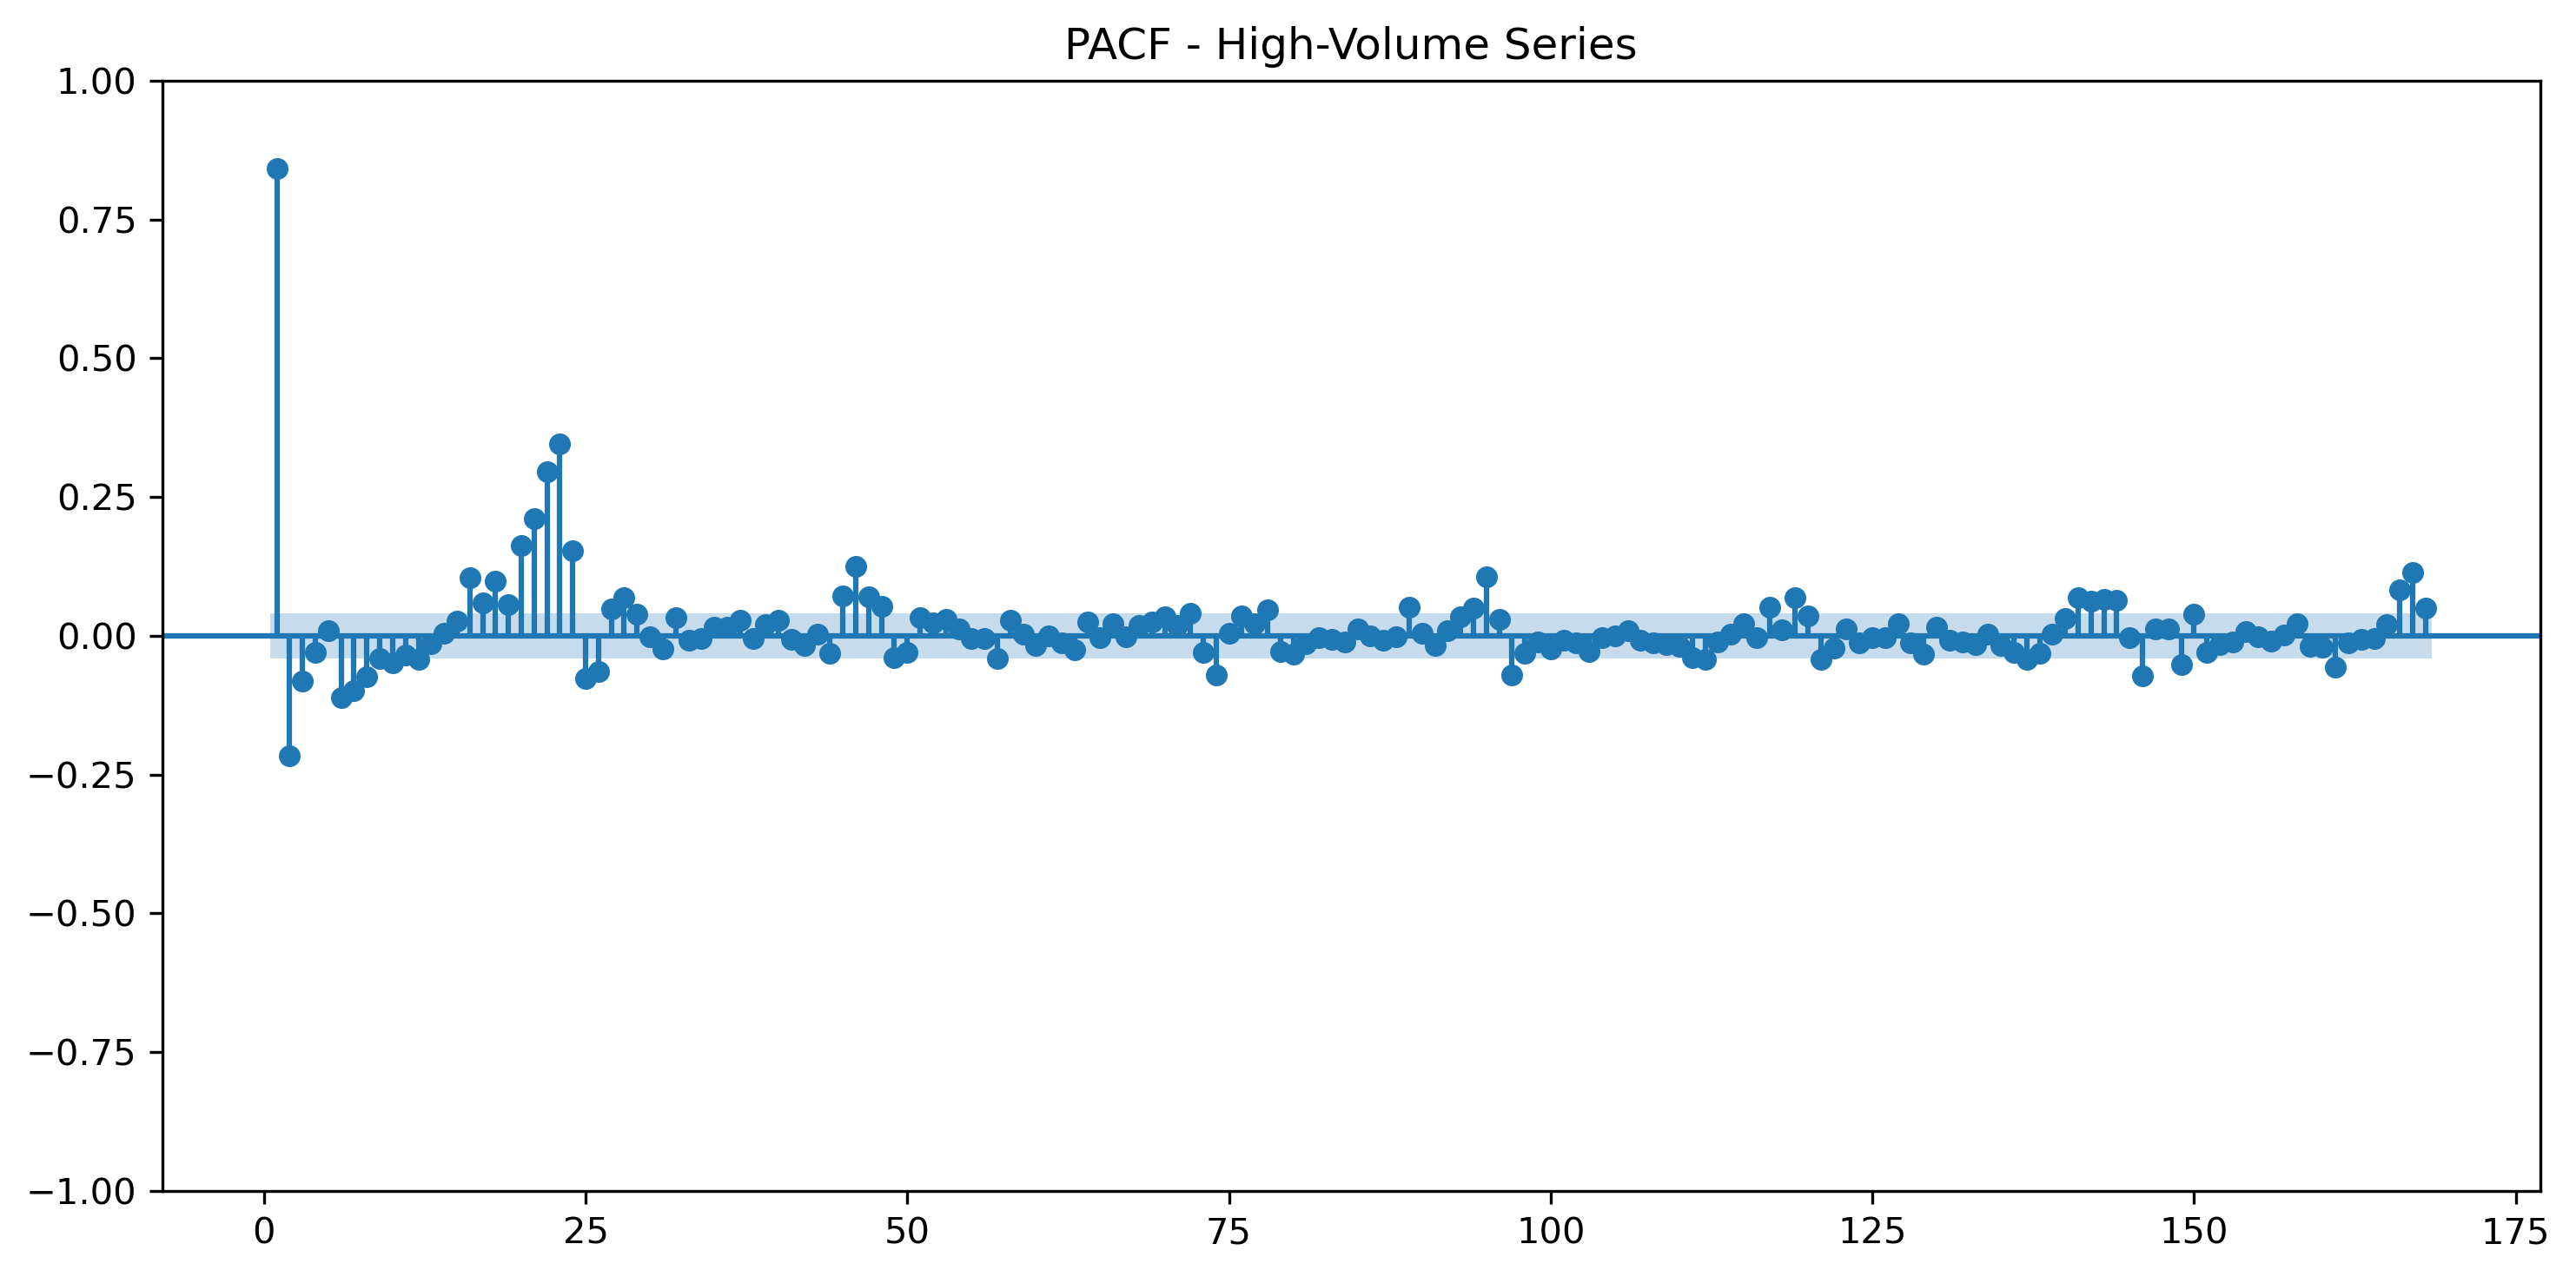
\includegraphics[width=0.84\linewidth]{figures/pacf_high_volume_series.png}
    \caption{PACF của chuỗi high-volume.}
    \label{fig:long-pacf-high}
\end{figure}


\subsection{Spectrum analysis}

Periodogram được dùng như một cách kiểm tra độc lập trong miền tần số. Hourly aggregate sales có peak mạnh quanh 24 giờ, còn daily recovered demand có peak gần 7 ngày. Điều này giải thích vì sao seasonal naive 7 ngày không phải baseline yếu mà là benchmark rất khó đánh bại.


\begin{figure}[H]
    \centering
    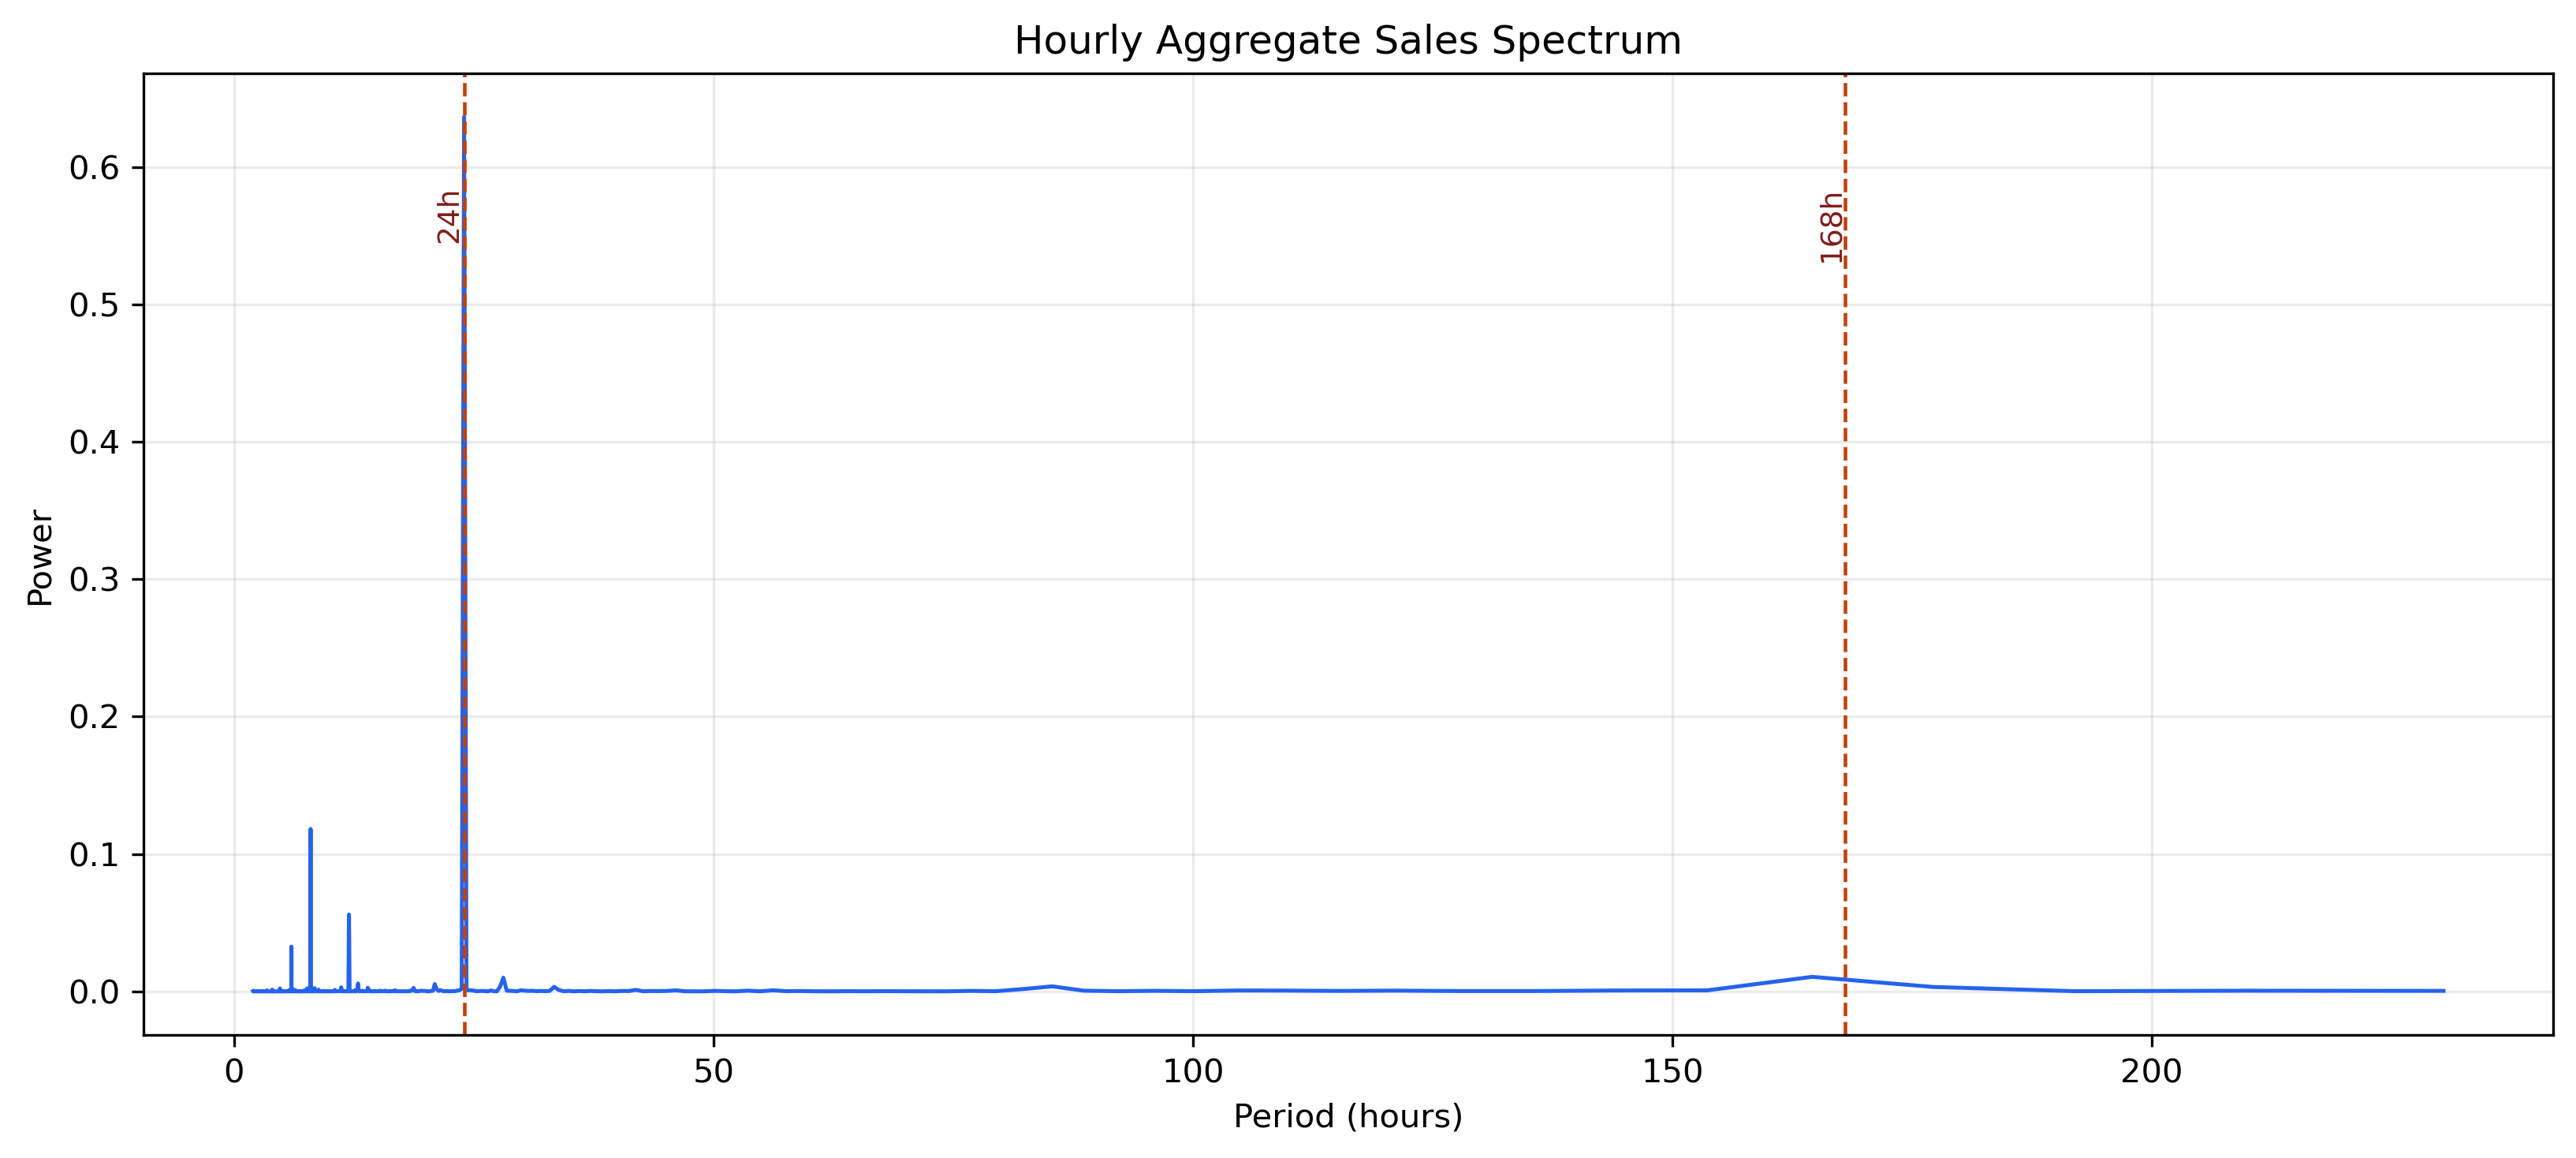
\includegraphics[width=0.86\linewidth]{figures/spectrum_hourly_aggregate_sales.png}
    \caption{Spectrum của hourly aggregate observed sales.}
    \label{fig:long-spectrum-hourly}
\end{figure}



\begin{table}[H]
\centering
\caption{Các peak spectrum hourly}
\label{tab:long-spectrum-hourly}
\resizebox{\linewidth}{!}{%
\begin{tabular}{lllll}
\toprule
Rank & Period & Frequency & Power & Period unit \\
\midrule
1 & 24.0000 & 0.0417 & 0.6365 & hours \\
2 & 8.0000 & 0.1250 & 0.1182 & hours \\
3 & 12.0000 & 0.0833 & 0.0559 & hours \\
4 & 6.0000 & 0.1667 & 0.0325 & hours \\
5 & 164.5714 & 0.0061 & 0.0106 & hours \\
6 & 28.0976 & 0.0356 & 0.0099 & hours \\
7 & 12.9438 & 0.0773 & 0.0058 & hours \\
8 & 20.9455 & 0.0477 & 0.0053 & hours \\
\bottomrule
\end{tabular}
}
\end{table}



\begin{figure}[H]
    \centering
    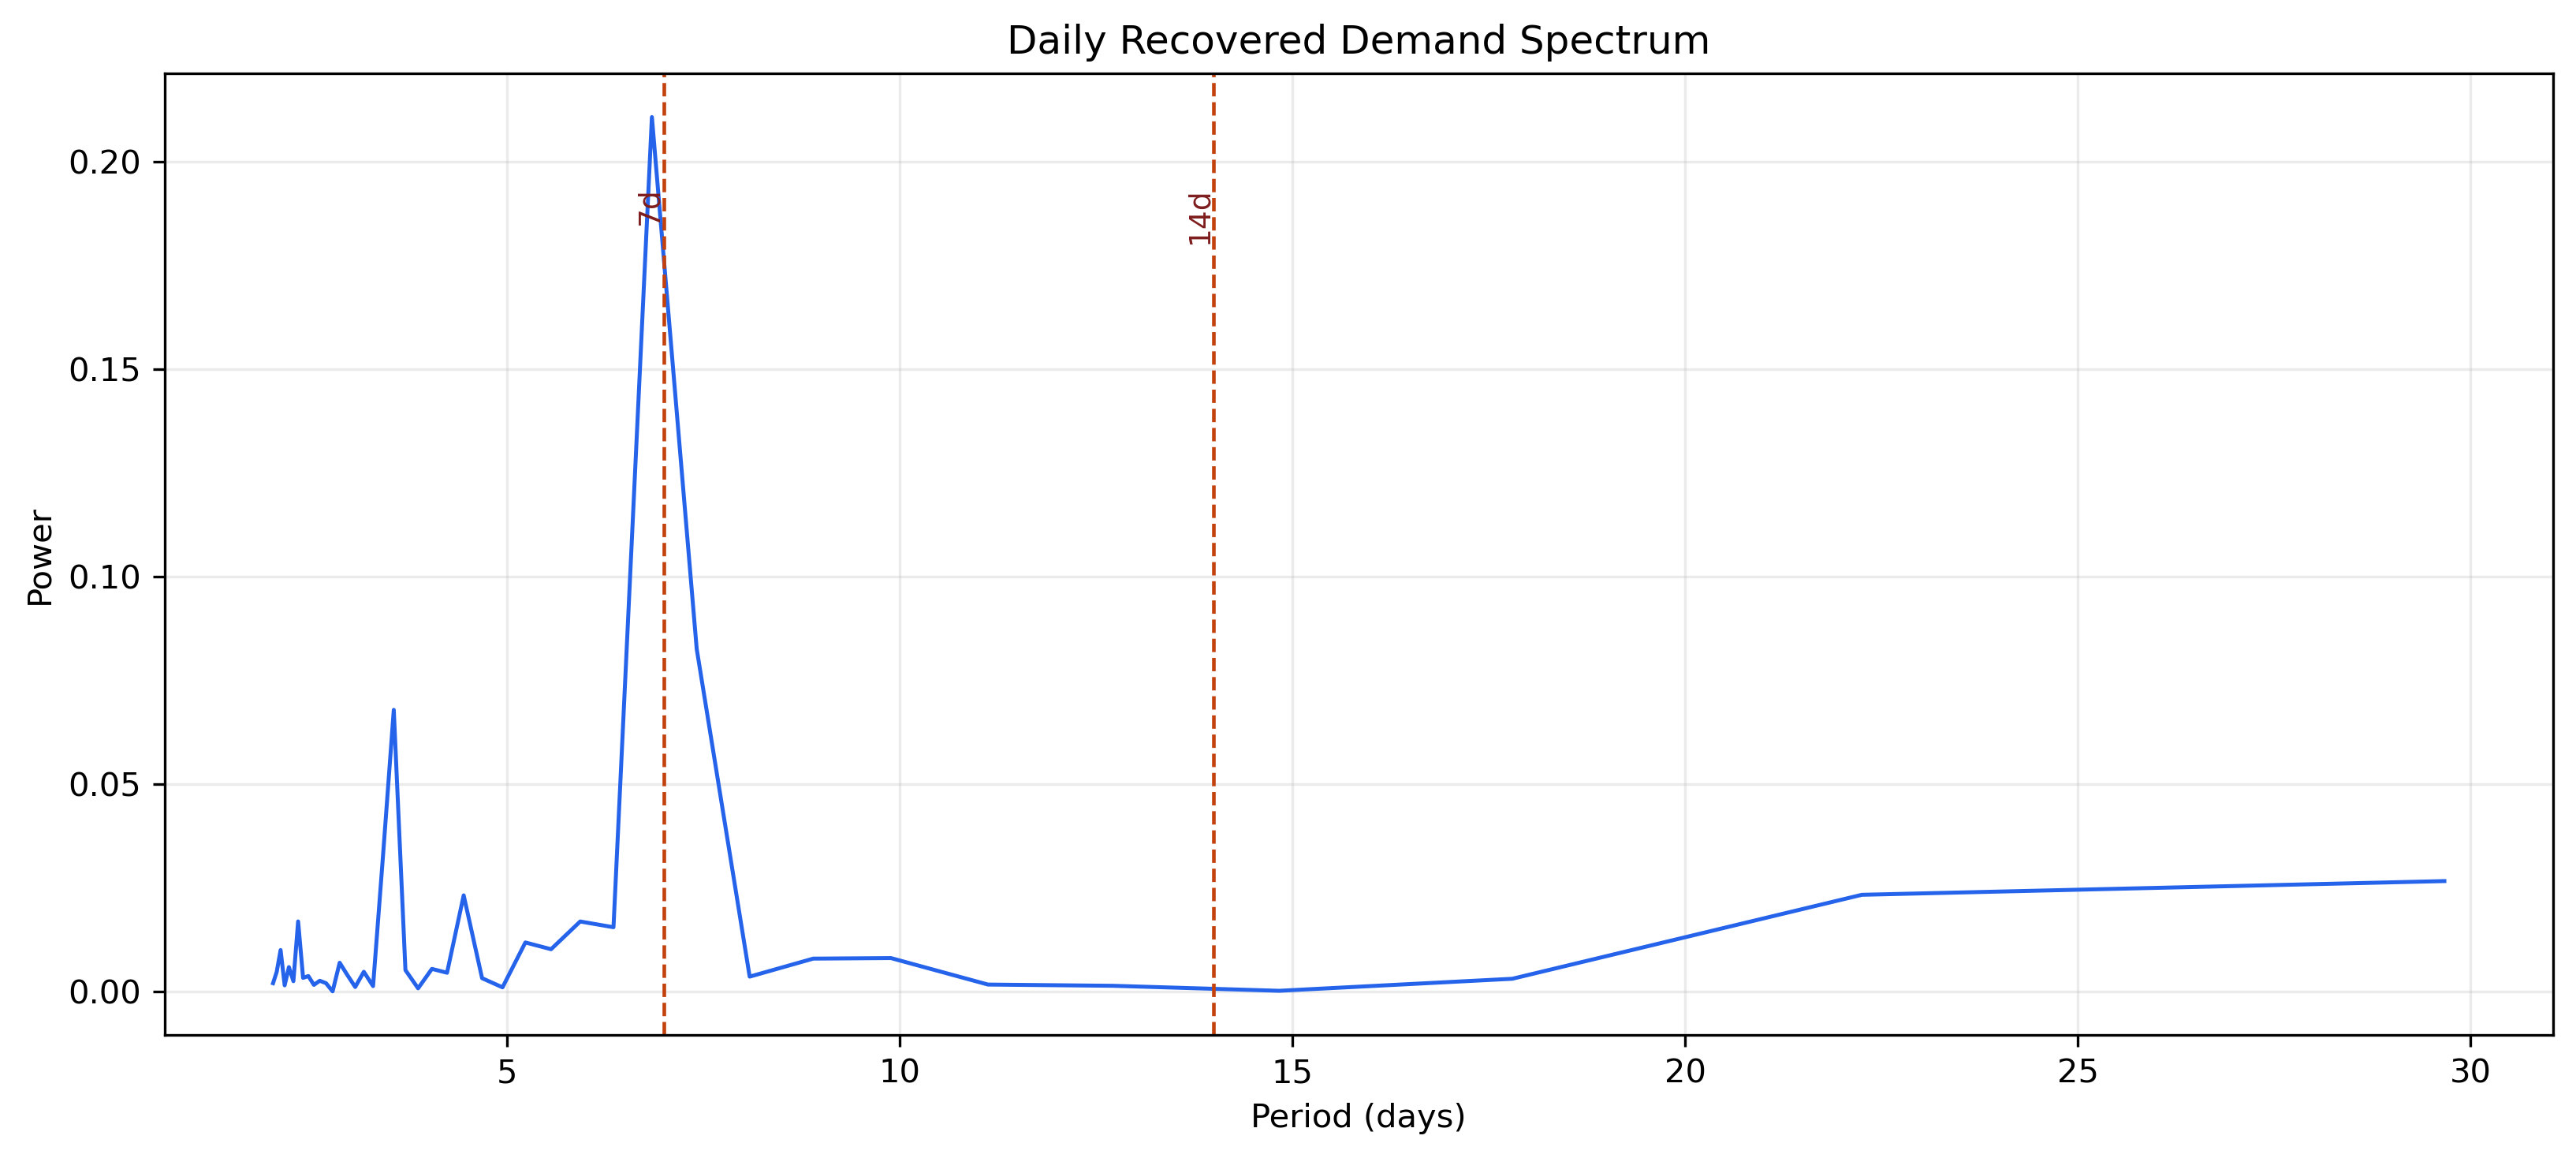
\includegraphics[width=0.86\linewidth]{figures/spectrum_daily_recovered_demand.png}
    \caption{Spectrum của daily recovered demand.}
    \label{fig:long-spectrum-daily}
\end{figure}



\begin{table}[H]
\centering
\caption{Các peak spectrum daily}
\label{tab:long-spectrum-daily}
\resizebox{\linewidth}{!}{%
\begin{tabular}{lllll}
\toprule
Rank & Period & Frequency & Power & Period unit \\
\midrule
1 & 6.8462 & 0.1461 & 0.2108 & days \\
2 & 3.5600 & 0.2809 & 0.0679 & days \\
3 & 4.4500 & 0.2247 & 0.0232 & days \\
4 & 2.3421 & 0.4270 & 0.0169 & days \\
5 & 5.9333 & 0.1685 & 0.0169 & days \\
6 & 5.2353 & 0.1910 & 0.0118 & days \\
7 & 2.1190 & 0.4719 & 0.0100 & days \\
8 & 9.8889 & 0.1011 & 0.0081 & days \\
\bottomrule
\end{tabular}
}
\end{table}

\section{Phương pháp}

\subsection{Vì sao không forecast observed sales trực tiếp?}

Observed sales là biến có thể bị censor bởi tồn kho. Trong giờ stockout, doanh số quan sát được là phần bán được trước khi hết hàng hoặc bằng không, không nhất thiết bằng demand thật. Nếu train model trực tiếp trên observed sales, mô hình có thể học rằng các chuỗi thường hết hàng có demand thấp. Điều này dẫn đến under-forecast và quyết định replenishment thiếu hàng.

\subsection{Two-stage framework}

Pipeline chính gồm hai stage. Stage 1 recover latent demand ở cấp hourly cho các giờ stockout. Stage 2 aggregate hourly recovered demand lên daily và forecast tổng nhu cầu 7 ngày tiếp theo. Cách này giữ thông tin stockout chi tiết ở nơi nó xuất hiện, nhưng trả forecast cuối ở cấp daily phù hợp hơn cho quyết định vận hành.


\begin{figure}[H]
    \centering
    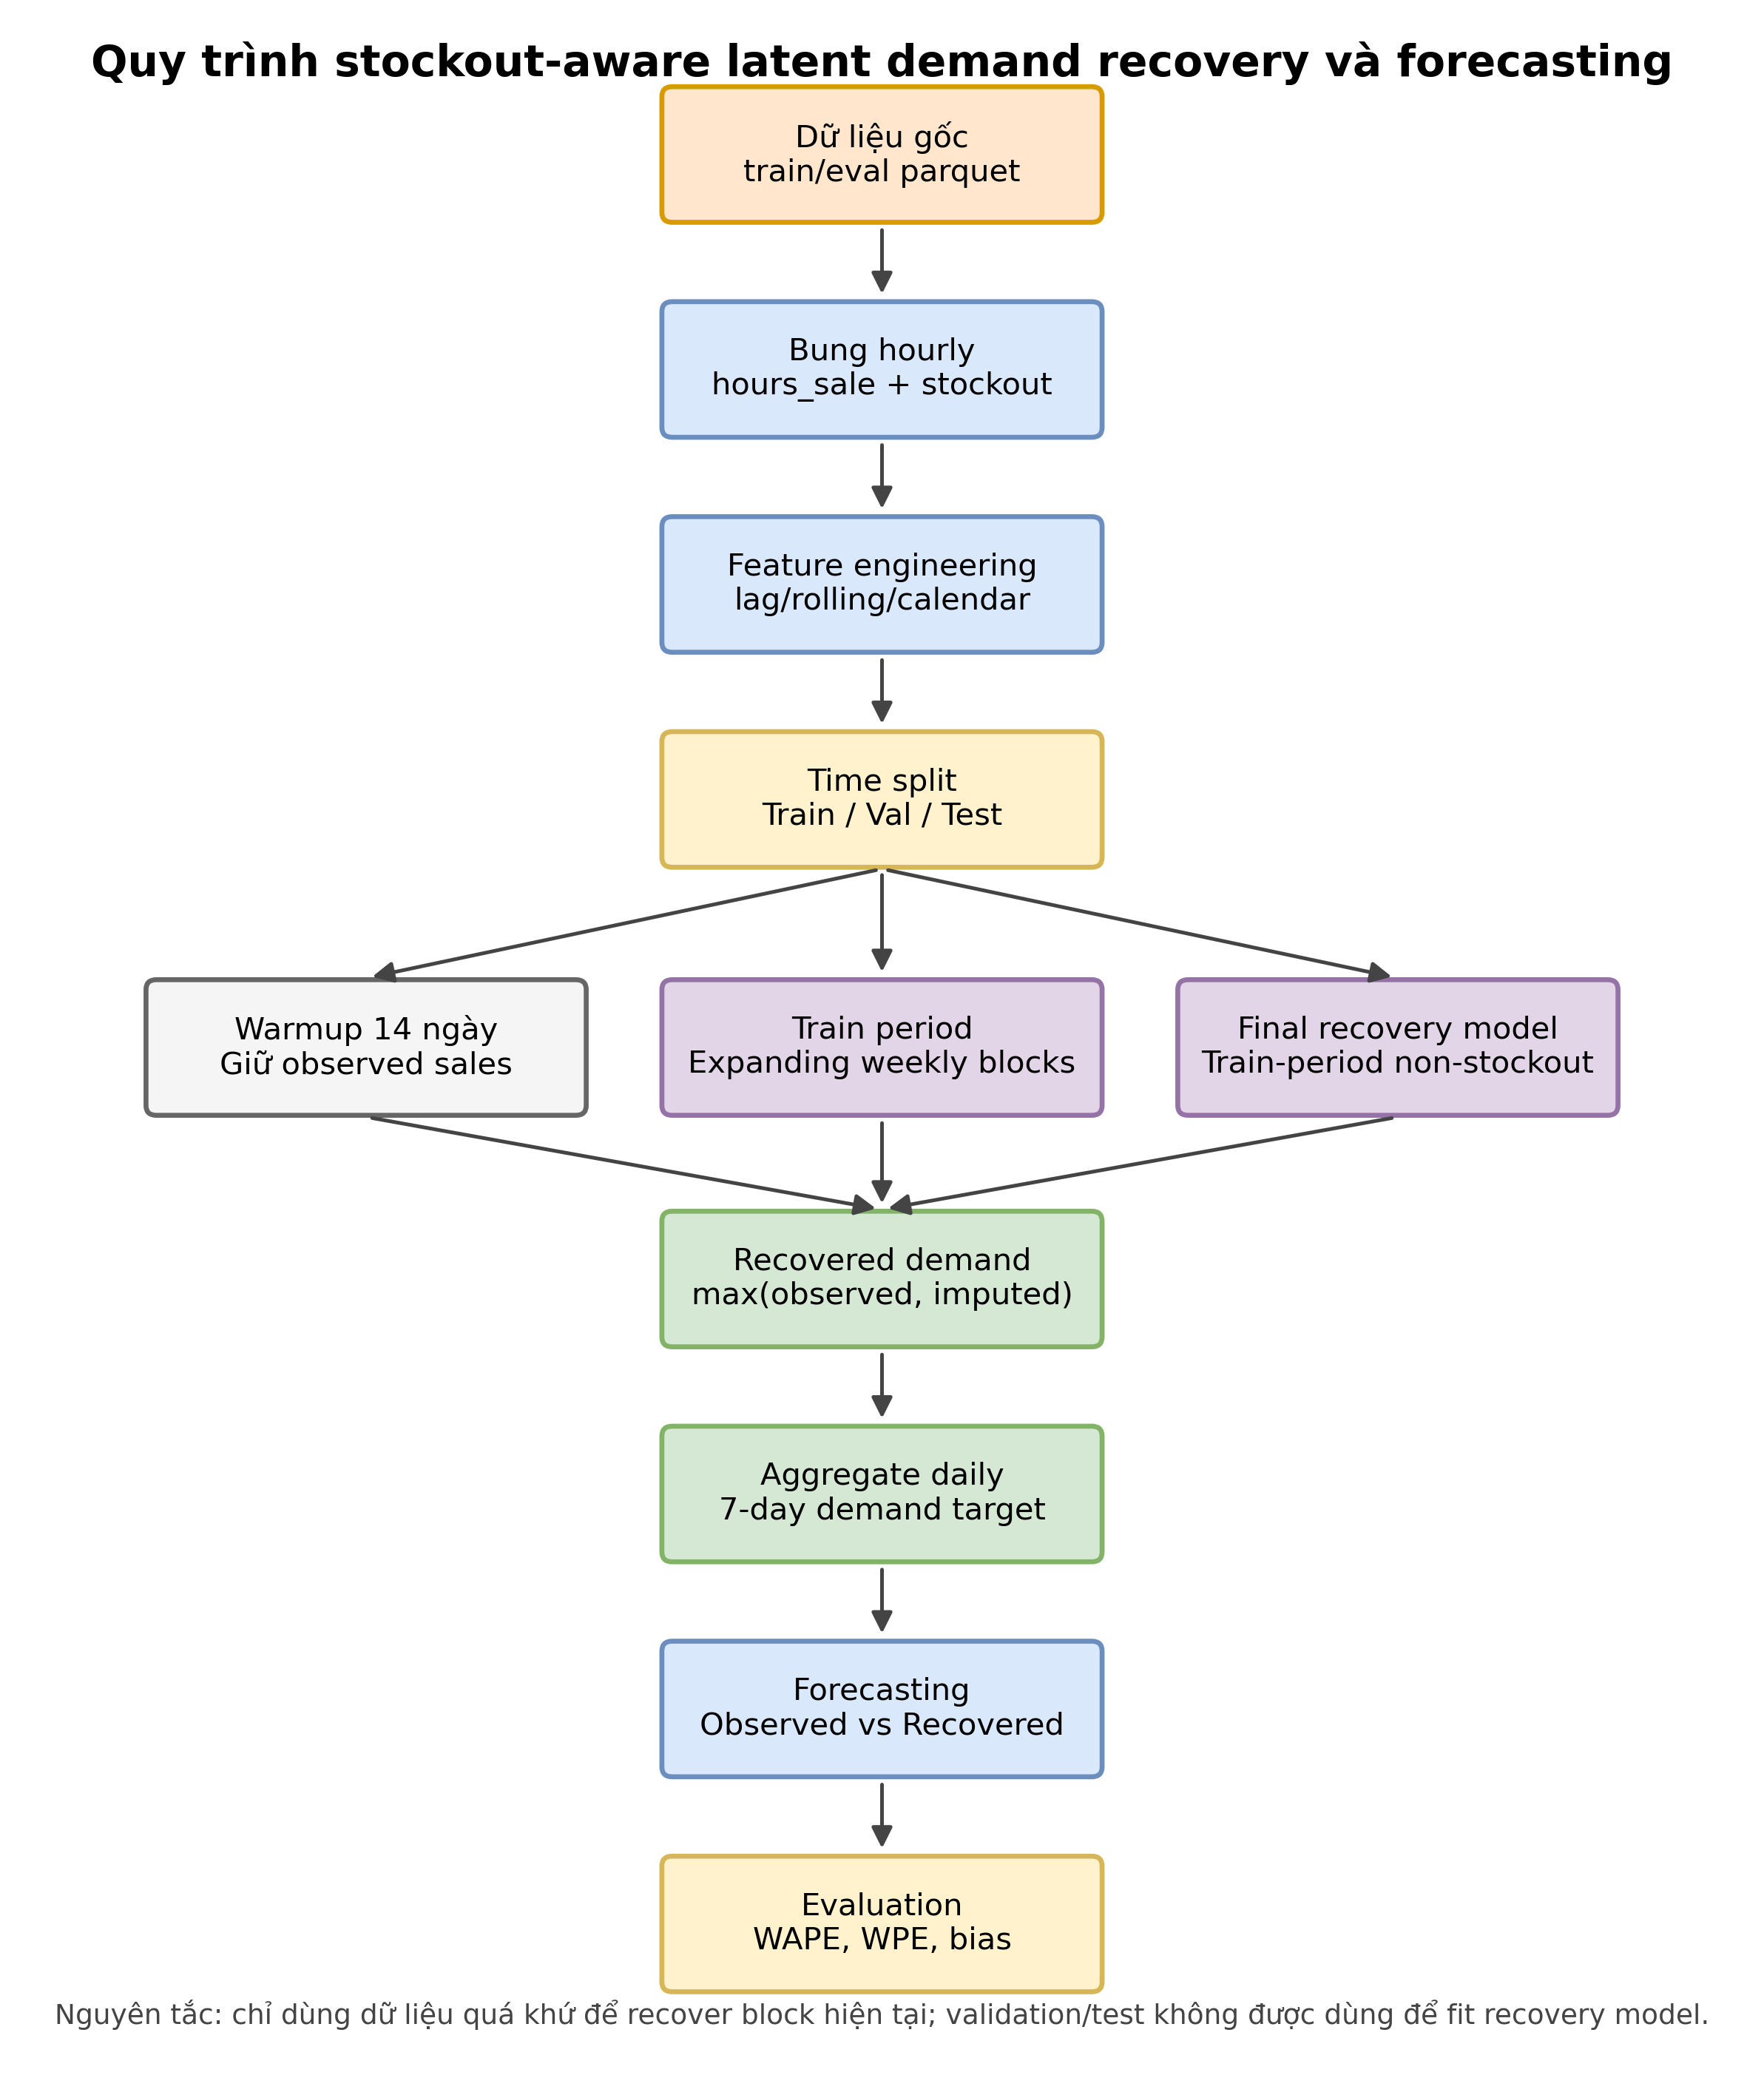
\includegraphics[width=0.88\linewidth]{figures/owner_expanding_window_process.png}
    \caption{Quy trình tổng quát two-stage.}
    \label{fig:long-process}
\end{figure}


\subsection{Expanding-window recovery}

Điểm dễ gây leakage nhất là latent demand recovery. Nếu dùng dữ liệu tương lai để impute quá khứ, forecast sau đó sẽ quá lạc quan. Vì vậy, trong train period, recovery được thực hiện theo block 7 ngày: mỗi block chỉ được recover bằng model học từ non-stockout rows nằm trước block đó. Validation/test được recover bằng final recovery model train trên non-stockout rows của train period.


\begin{figure}[H]
    \centering
    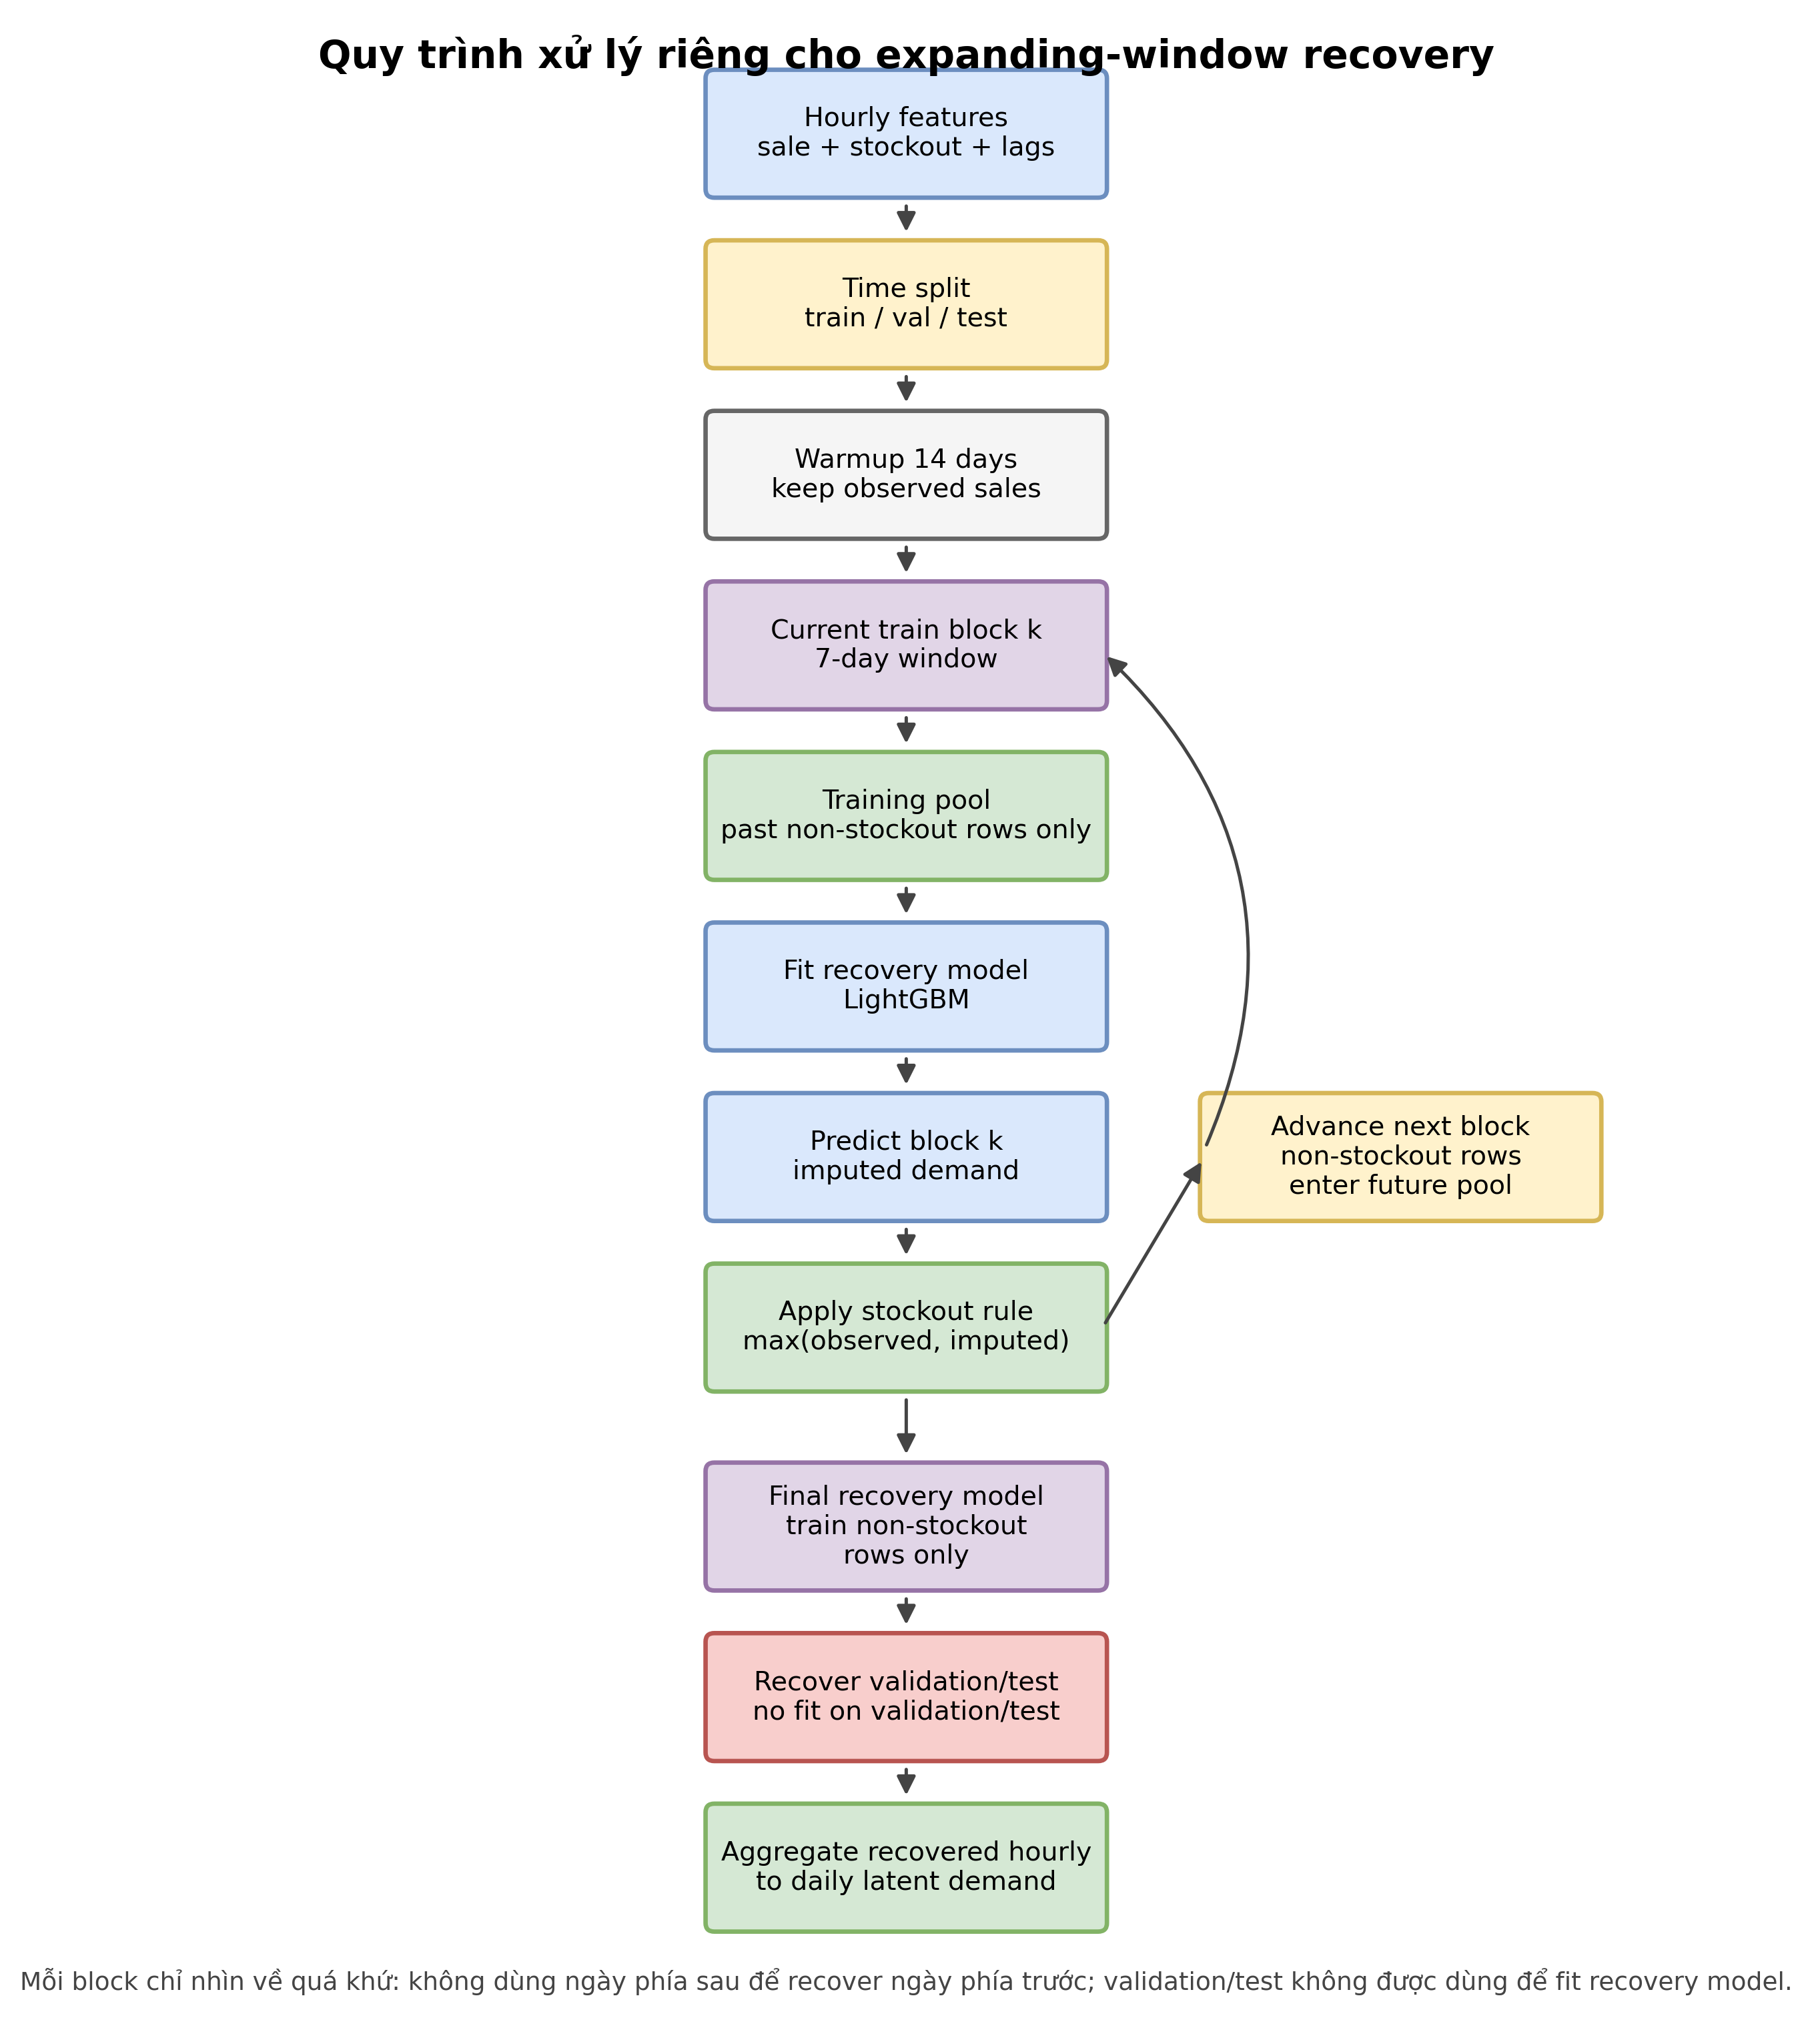
\includegraphics[width=0.90\linewidth]{figures/owner_expanding_window_recovery_detail.png}
    \caption{Chi tiết expanding-window recovery.}
    \label{fig:long-recovery-detail}
\end{figure}


\subsection{Calibration và cap}

Raw imputed demand có thể overpredict. Do đó, dự đoán raw được hiệu chỉnh bằng calibration factor học từ validation non-stockout rows. Sau đó lost demand dương được cap ở q90 để tránh một số giờ stockout cực trị làm tổng demand tăng quá mức. Công thức triển khai là:

\[
\text{lost}_t = \max\left(\frac{\hat{y}^{raw}_t}{c} - y^{obs}_t, 0\right),
\quad
\text{lost}^{cap}_t = \min(\text{lost}_t, q90),
\quad
y^{rec}_t = y^{obs}_t + \text{lost}^{cap}_t.
\]

\subsection{Daily forecasting target}

Sau recovery hourly, dữ liệu được aggregate lên daily. Target chính là \texttt{target\_next7\_recovered\_daily}, tức tổng recovered demand trong 7 ngày sau forecast origin. Target dạng tổng 7 ngày phù hợp với bài toán replenishment hơn forecast từng giờ riêng lẻ vì quyết định nhập hàng thường dựa trên nhu cầu vài ngày tới.

\subsection{Modeling choice}

LightGBM được chọn vì đây là bài toán tabular time-series quy mô lớn với nhiều feature lag, rolling, calendar, stockout, promotion và weather. Classical ARIMA/SARIMA không được chọn làm model chính vì khó scale tới hàng nghìn chuỗi store-product và khó xử lý chuỗi thưa. Deep learning không phải trọng tâm vì yêu cầu tuning/tài nguyên cao hơn, trong khi mục tiêu đồ án là một pipeline có thể giải thích và tái lập.

\subsection{Baselines và hybrid}

Báo cáo không chỉ so sánh hai mô hình ML. Các baseline daily gồm naive x7, seasonal naive 7-day và rolling mean 14-day. Seasonal naive 7-day rất mạnh do dữ liệu có seasonality tuần rõ. Vì vậy, mô hình cuối là hybrid seasonal-ML: blend giữa seasonal naive 7-day và recovered-demand LightGBM, với trọng số chọn trên validation set.

\section{Latent demand recovery và kiểm soát imputation}

\subsection{Kết quả recovery tổng quan}

Bảng sau tóm tắt kết quả recovery. Recovered demand tăng khoảng 10.68\% so với observed sales. Về business, con số này có thể hiểu là phần demand tiềm ẩn mà observed sales không phản ánh đầy đủ do stockout.


\begin{table}[H]
\centering
\caption{Tóm tắt latent demand recovery}
\label{tab:long-recovery-summary}
\resizebox{\linewidth}{!}{%
\begin{tabular}{ll}
\toprule
Metric & Value \\
\midrule
Observed sales & 482697.09375 \\
Recovered latent demand & 534270.1875 \\
Recovered lost demand & 51572.875 \\
Recovered lift over observed & 0.10684314370155334 \\
Stockout row rate & 0.24652109375 \\
Recovery method & expanding-window weekly recovery \\
Imputation calibration factor & 1.1297638401922185 \\
Lost demand cap quantile & q90 of calibrated positive lost demand \\
Lost demand cap value & 0.06627678871154785 \\
Warmup days kept observed & 14 \\
Recovery block days & 7 \\
Recovery blocks & 9 \\
Final recovery train rows & 400000 \\
Recovery train source & past non-stockout rows only for train blocks; train-period non-stockout rows for validation/test \\
Final recovery train end & 2024-06-10 23:00:00 \\
Validation start & 2024-06-11 00:00:00 \\
Test start & 2024-06-18 00:00:00 \\
\bottomrule
\end{tabular}
}
\end{table}



\begin{figure}[H]
    \centering
    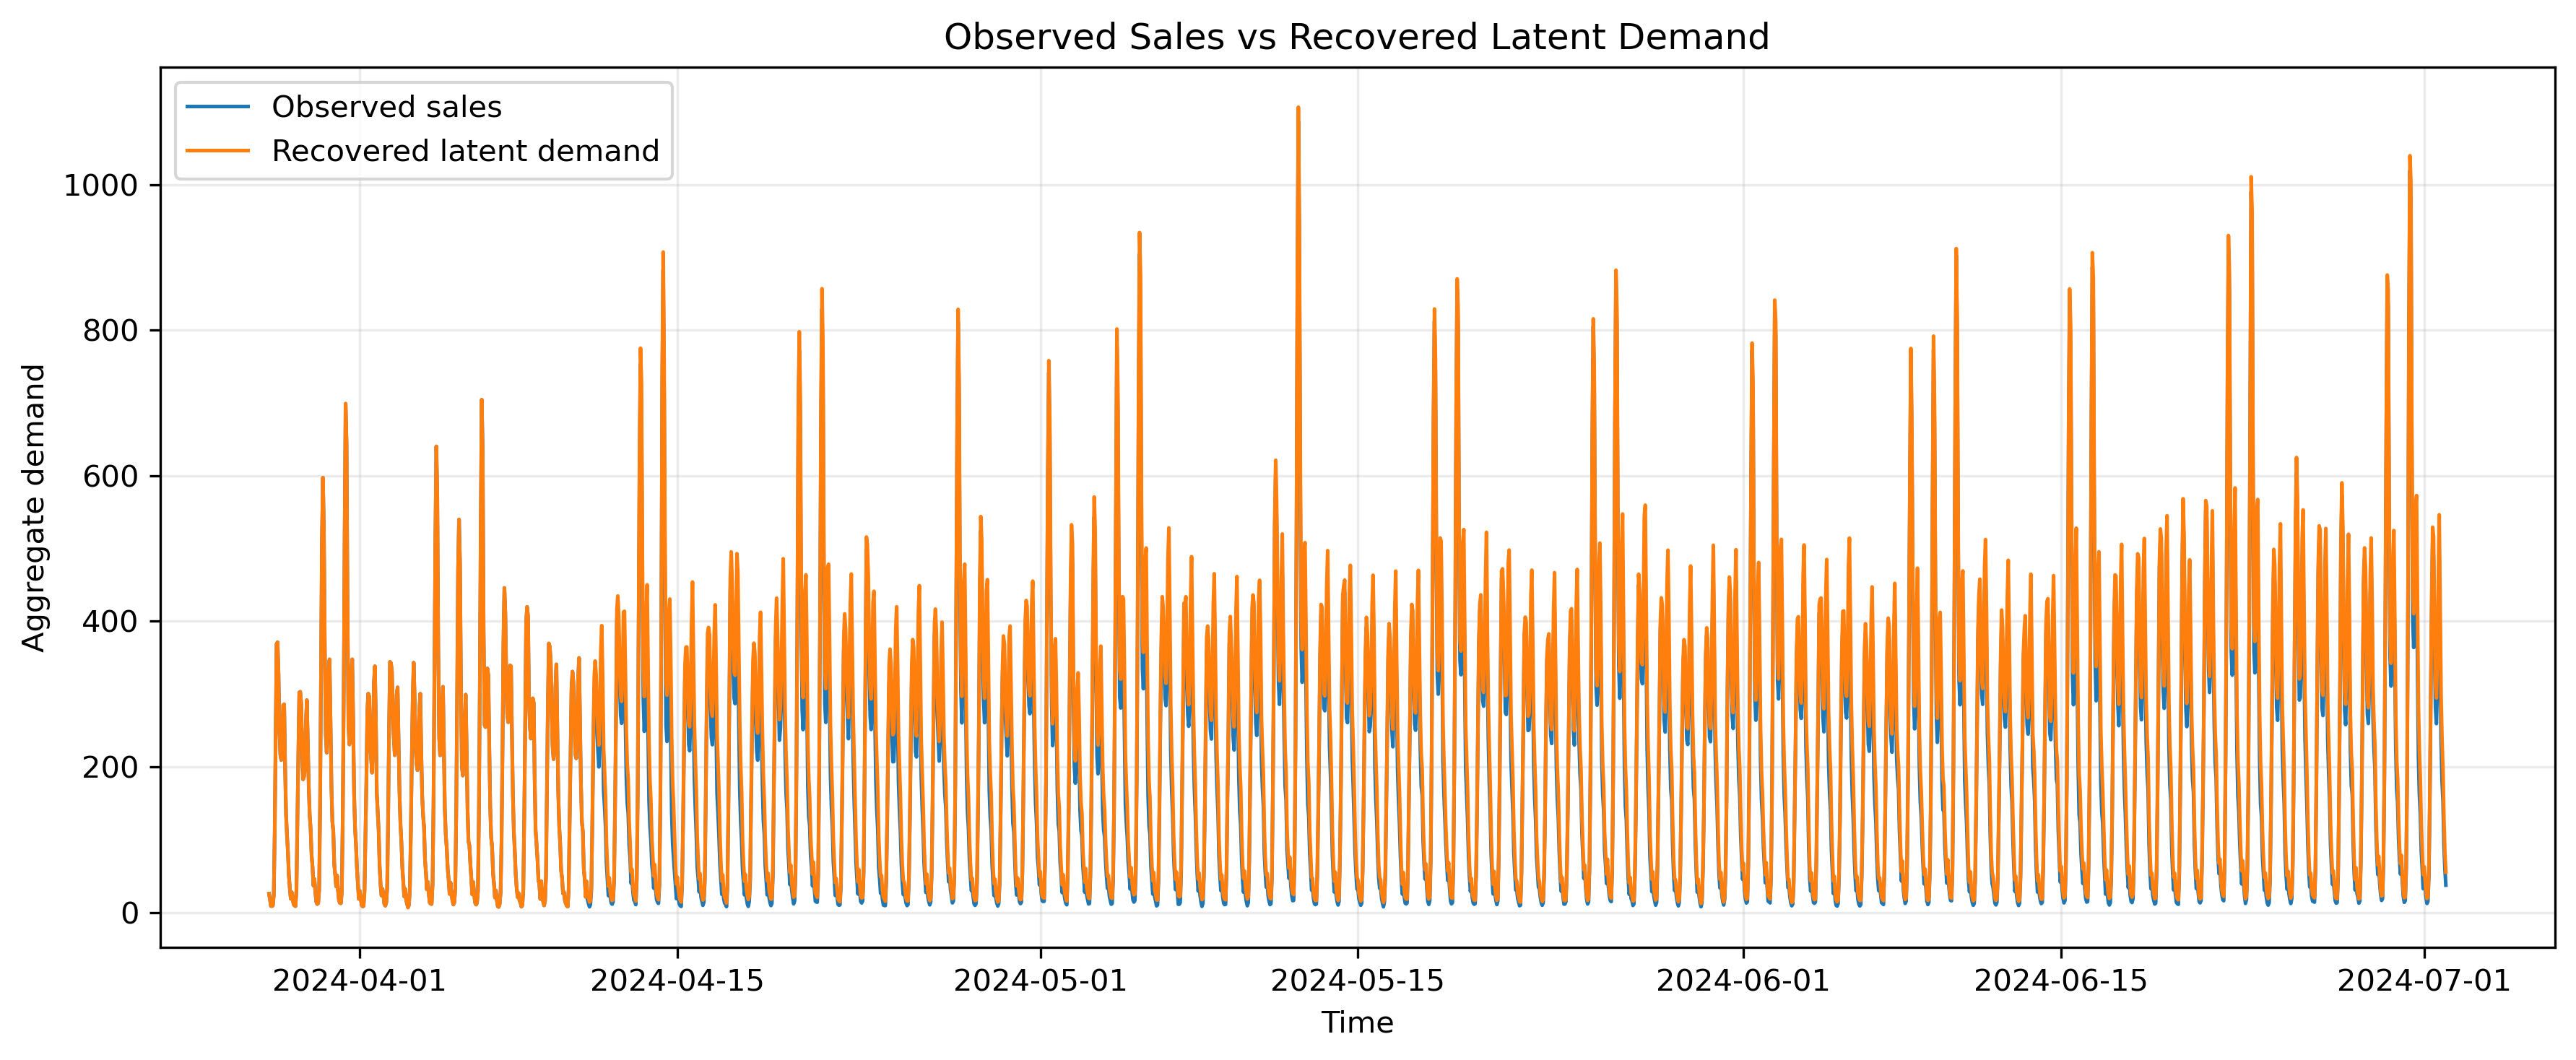
\includegraphics[width=0.92\linewidth]{figures/owner_observed_vs_recovered_demand.png}
    \caption{Observed sales và recovered demand theo thời gian.}
    \label{fig:long-observed-recovered}
\end{figure}


\subsection{Uplift do imputation}

Vì recovered demand không phải ground truth thật, báo cáo không dùng imputation một cách mù quáng. Uplift được kiểm tra ở nhiều cấp: tổng dataset, từng ngày và từng series. Nếu uplift quá lớn hoặc tập trung ở một số series, kết quả forecast sẽ phụ thuộc quá mạnh vào imputation.


\begin{table}[H]
\centering
\caption{Tổng mức uplift do imputation}
\label{tab:long-uplift}
\resizebox{0.86\linewidth}{!}{%
\begin{tabular}{ll}
\toprule
Metric & Value \\
\midrule
Observed sales & 482,697 \\
Recovered demand & 534,270 \\
Recovered lost demand & 51,573 \\
Recovered lift over observed & 0.1068 \\
Raw calibrated lost demand before cap & 65,368 \\
Cap retained share of raw lost demand & 0.7890 \\
Stockout row share & 0.2465 \\
Recovered lost demand from stockout rows & 51,573 \\
Mean stockout uplift per stockout row & 0.0182 \\
\bottomrule
\end{tabular}
}
\end{table}



\begin{figure}[H]
    \centering
    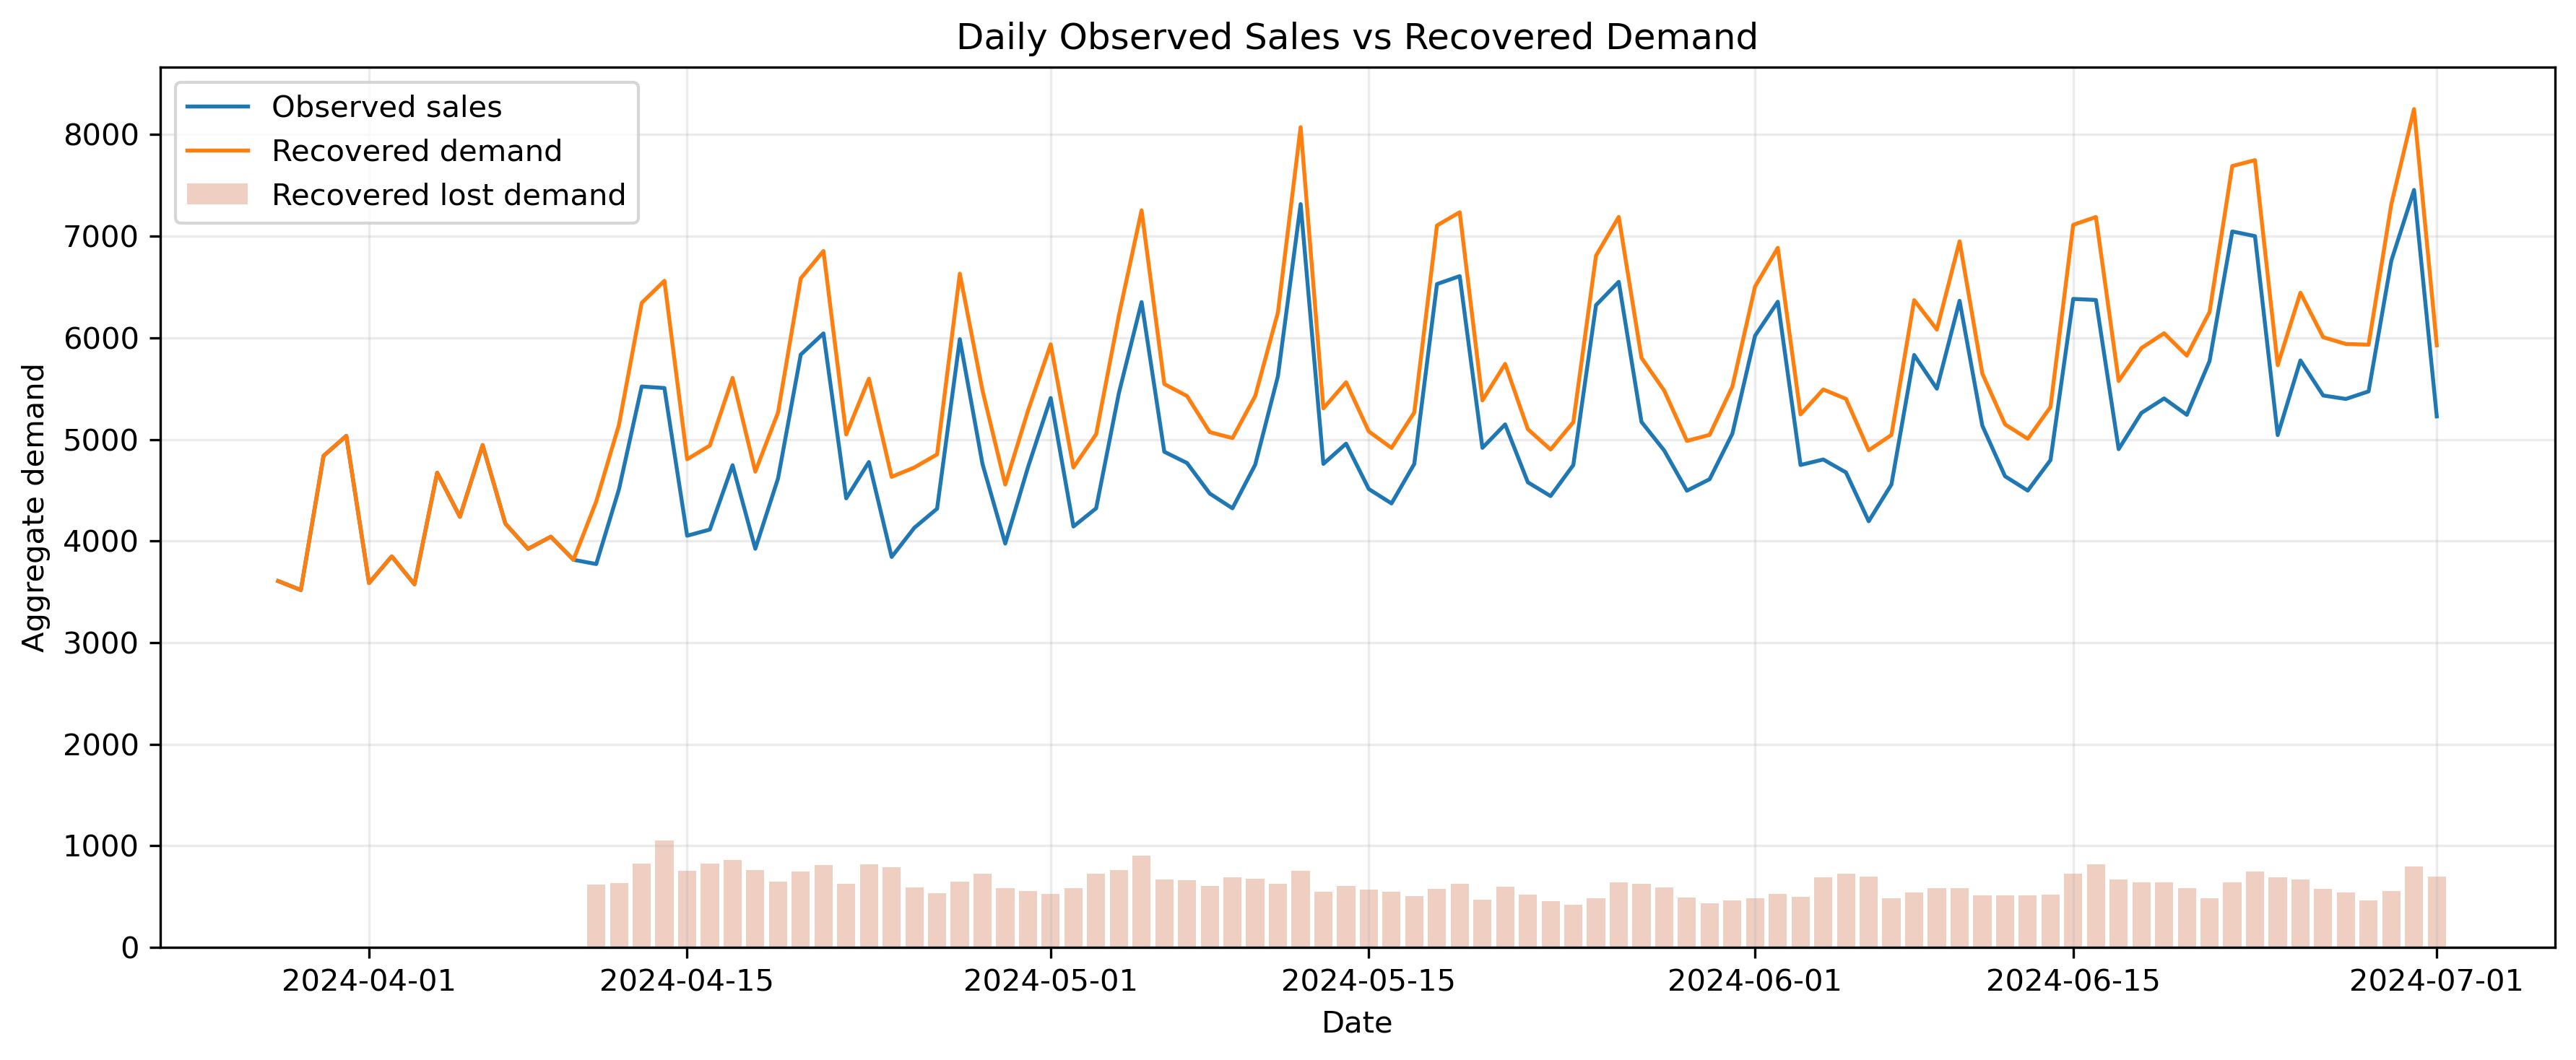
\includegraphics[width=0.92\linewidth]{figures/imputation_daily_uplift.png}
    \caption{Observed sales, recovered demand và recovered lost demand theo ngày.}
    \label{fig:long-daily-uplift}
\end{figure}


\subsection{Pseudo-stockout validation}

Pseudo-stockout validation lấy các dòng non-stockout trong validation period, giả sử chúng cần impute, rồi so sánh prediction của recovery model với observed sales thật. Row-level hourly validation có WAPE cao vì hourly sales rất thưa và nhiều giá trị nhỏ. Do đó, báo cáo bổ sung aggregate validation, phù hợp hơn với mục tiêu forecast daily demand.


\begin{table}[H]
\centering
\caption{Pseudo-stockout validation ở cấp row hourly}
\label{tab:long-pseudo-row}
\resizebox{0.86\linewidth}{!}{%
\begin{tabular}{ll}
\toprule
Metric & Value \\
\midrule
Validation rows & 300000 \\
Pseudo-stockout source & non-stockout rows from validation period \\
RMSE & 0.10030610859394073 \\
MAE & 0.05774029344320297 \\
WAPE & 1.0391554832458496 \\
sMAPE & 1.6277295807119518 \\
Mean prediction / actual ratio & 1.1315665245056152 \\
Mean error actual-minus-imputed & -0.007310444954782724 \\
\bottomrule
\end{tabular}
}
\end{table}



\begin{table}[H]
\centering
\caption{Pseudo-stockout validation ở các cấp aggregate}
\label{tab:long-pseudo-agg}
\resizebox{\linewidth}{!}{%
\begin{tabular}{lllllll}
\toprule
Validation level & RMSE & MAE & WAPE & sMAPE & Prediction / actual ratio & N \\
\midrule
Hourly aggregate & 42.5877 & 21.9068 & 0.2208 & 0.2237 & 1.1316 & 168 \\
Daily aggregate & 450.9920 & 416.6911 & 0.1750 & 0.1677 & 1.1316 & 7 \\
Series daily aggregate & 0.3245 & 0.2155 & 0.4384 & 0.6309 & 1.1316 & 33907 \\
\bottomrule
\end{tabular}
}
\end{table}


\subsection{Sensitivity theo cap}

Cap q90 được chọn như một điểm cân bằng. Cap q75 bảo thủ hơn nhưng có thể under-recover; q100 giữ toàn bộ raw lost demand nhưng dễ phụ thuộc mạnh vào outlier. Sensitivity giúp chứng minh kết luận không chỉ dựa trên một lựa chọn cap tùy tiện.


\begin{table}[H]
\centering
\caption{Sensitivity theo mức cap lost demand}
\label{tab:long-cap-sensitivity}
\resizebox{\linewidth}{!}{%
\begin{tabular}{llllll}
\toprule
Scenario & Cap value & Recovered demand & Recovered lost demand & Recovered lift over observed & Share of original recovered lost demand \\
\midrule
Cap lost-demand at q50 & 0.0151 & 505,963 & 23,266 & 0.0482 & 0.3559 \\
Cap lost-demand at q75 & 0.0369 & 523,781 & 41,084 & 0.0851 & 0.6285 \\
Cap lost-demand at q90 & 0.0663 & 534,270 & 51,573 & 0.1068 & 0.7890 \\
Cap lost-demand at q100 & 2.7508 & 548,064 & 65,368 & 0.1354 & 1.0000 \\
\bottomrule
\end{tabular}
}
\end{table}



\begin{figure}[H]
    \centering
    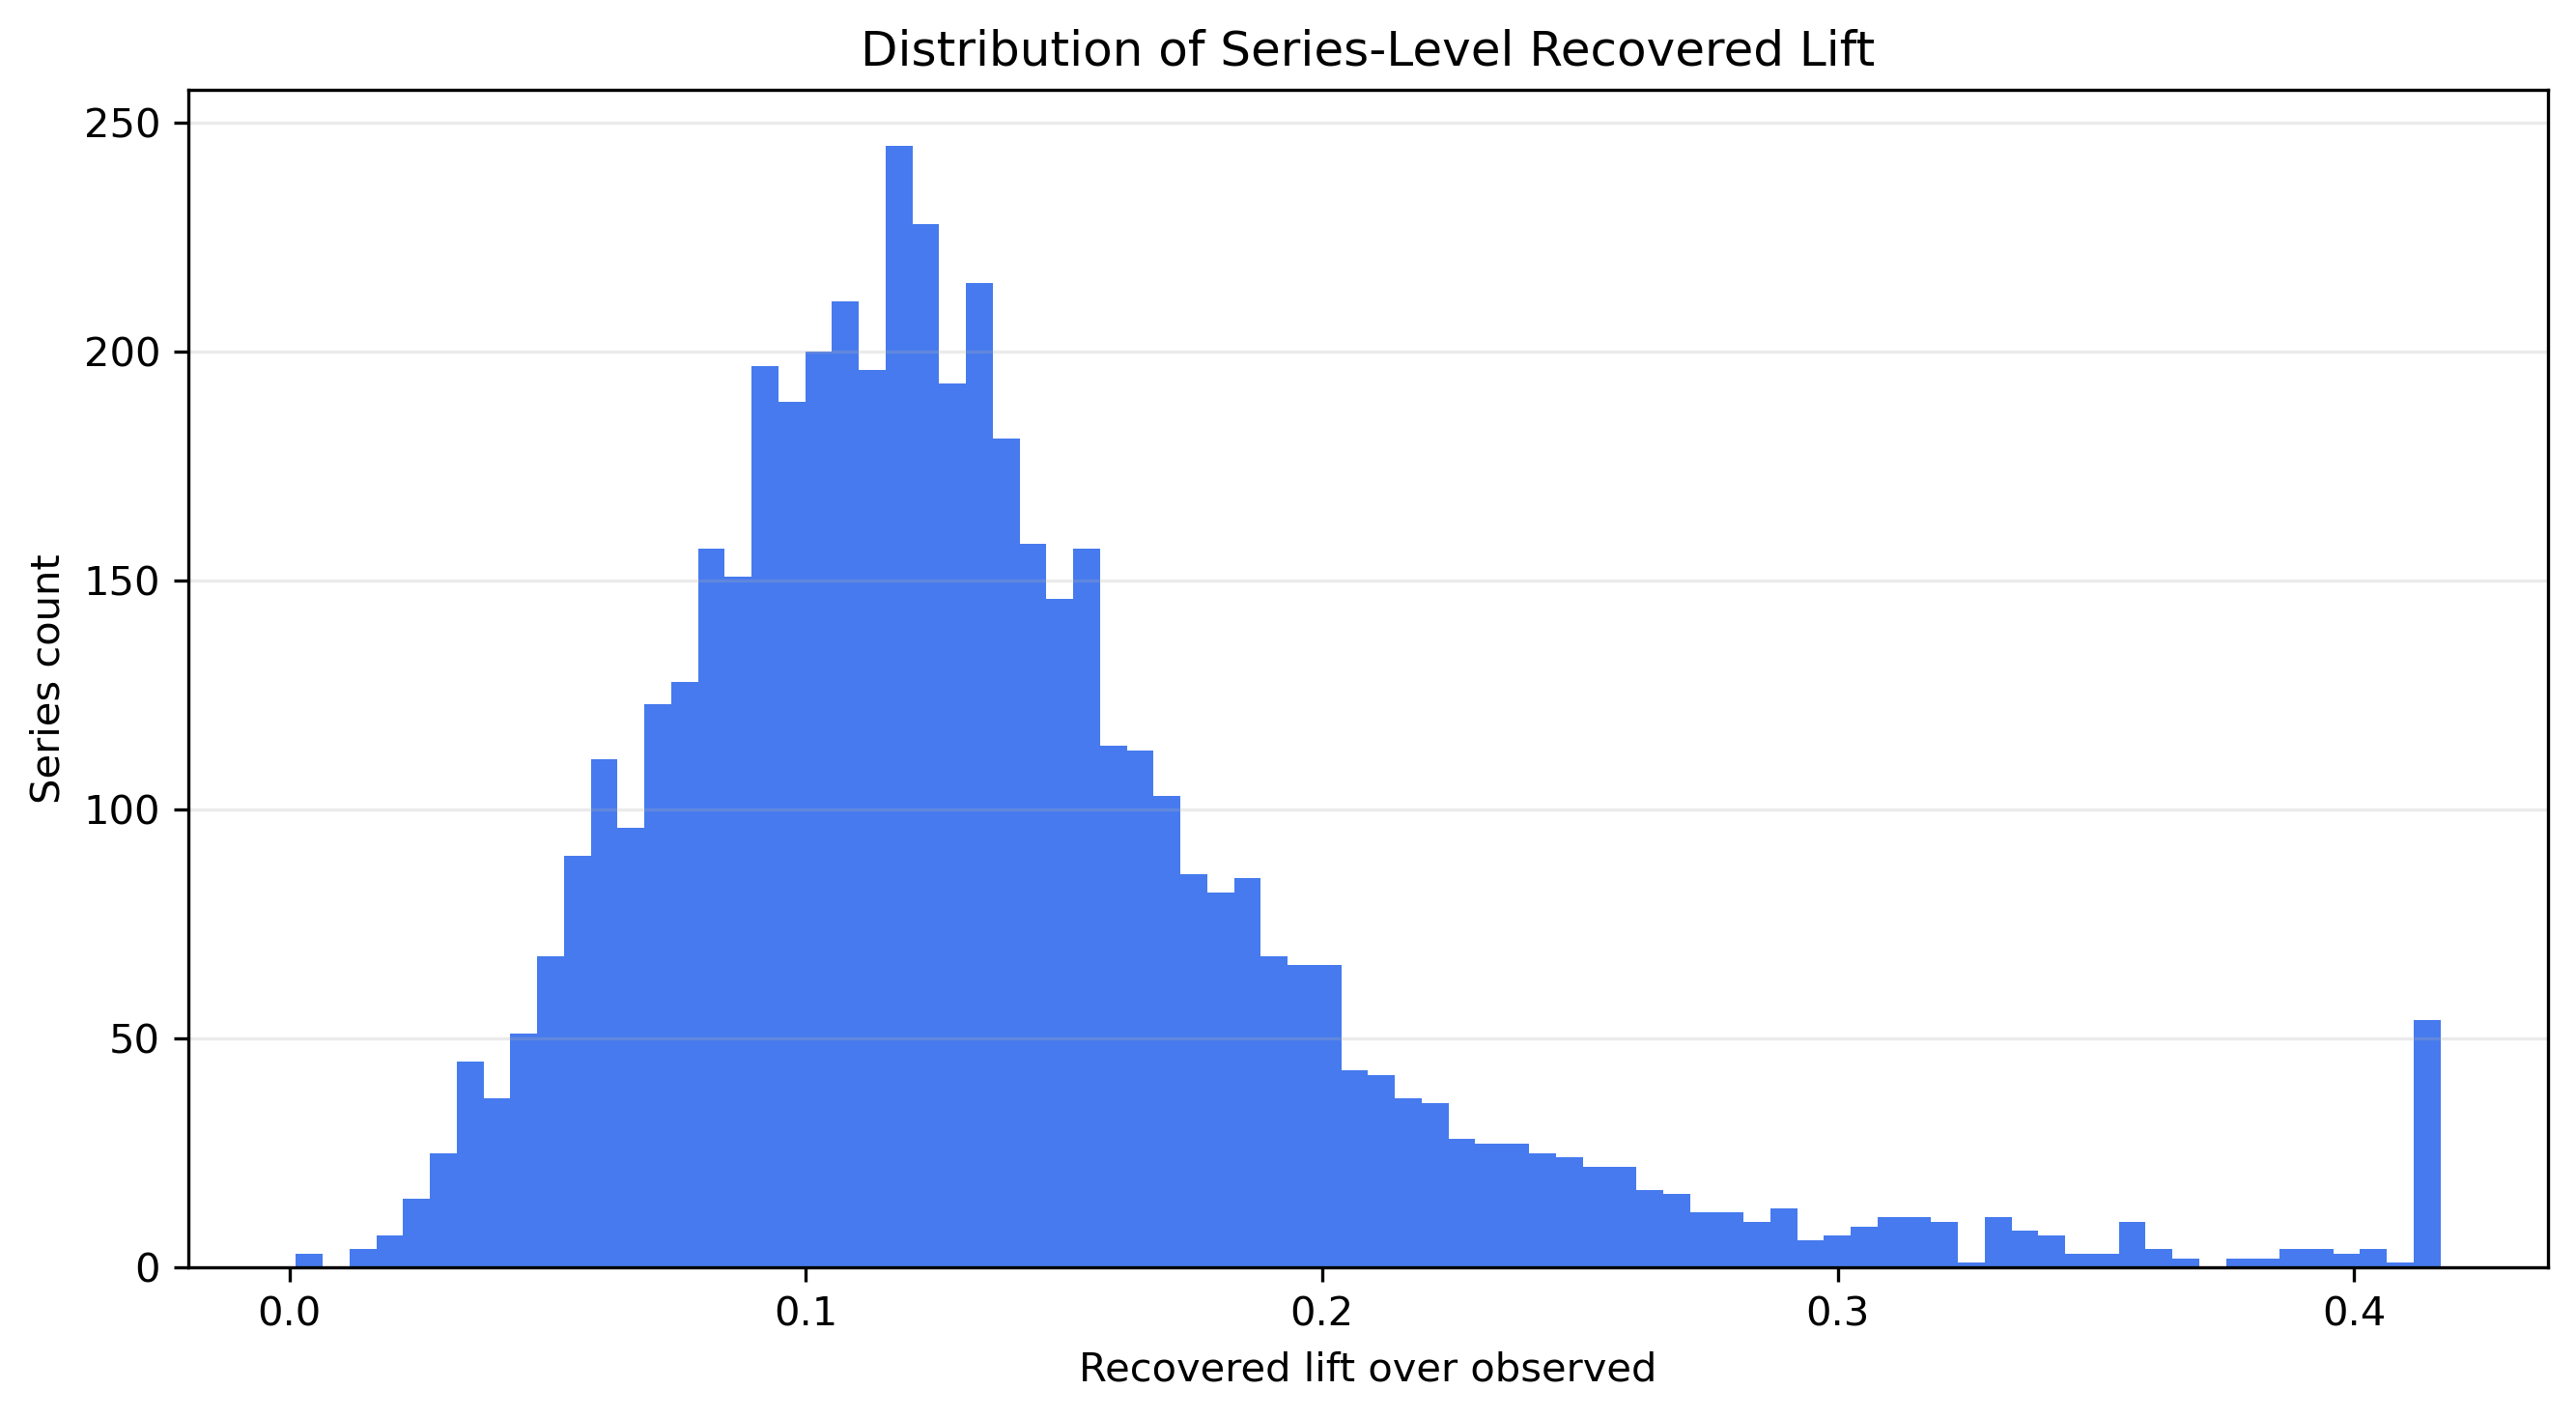
\includegraphics[width=0.78\linewidth]{figures/imputation_series_lift_distribution.png}
    \caption{Phân phối recovered lift ở cấp series.}
    \label{fig:long-lift-dist}
\end{figure}



\begin{figure}[H]
    \centering
    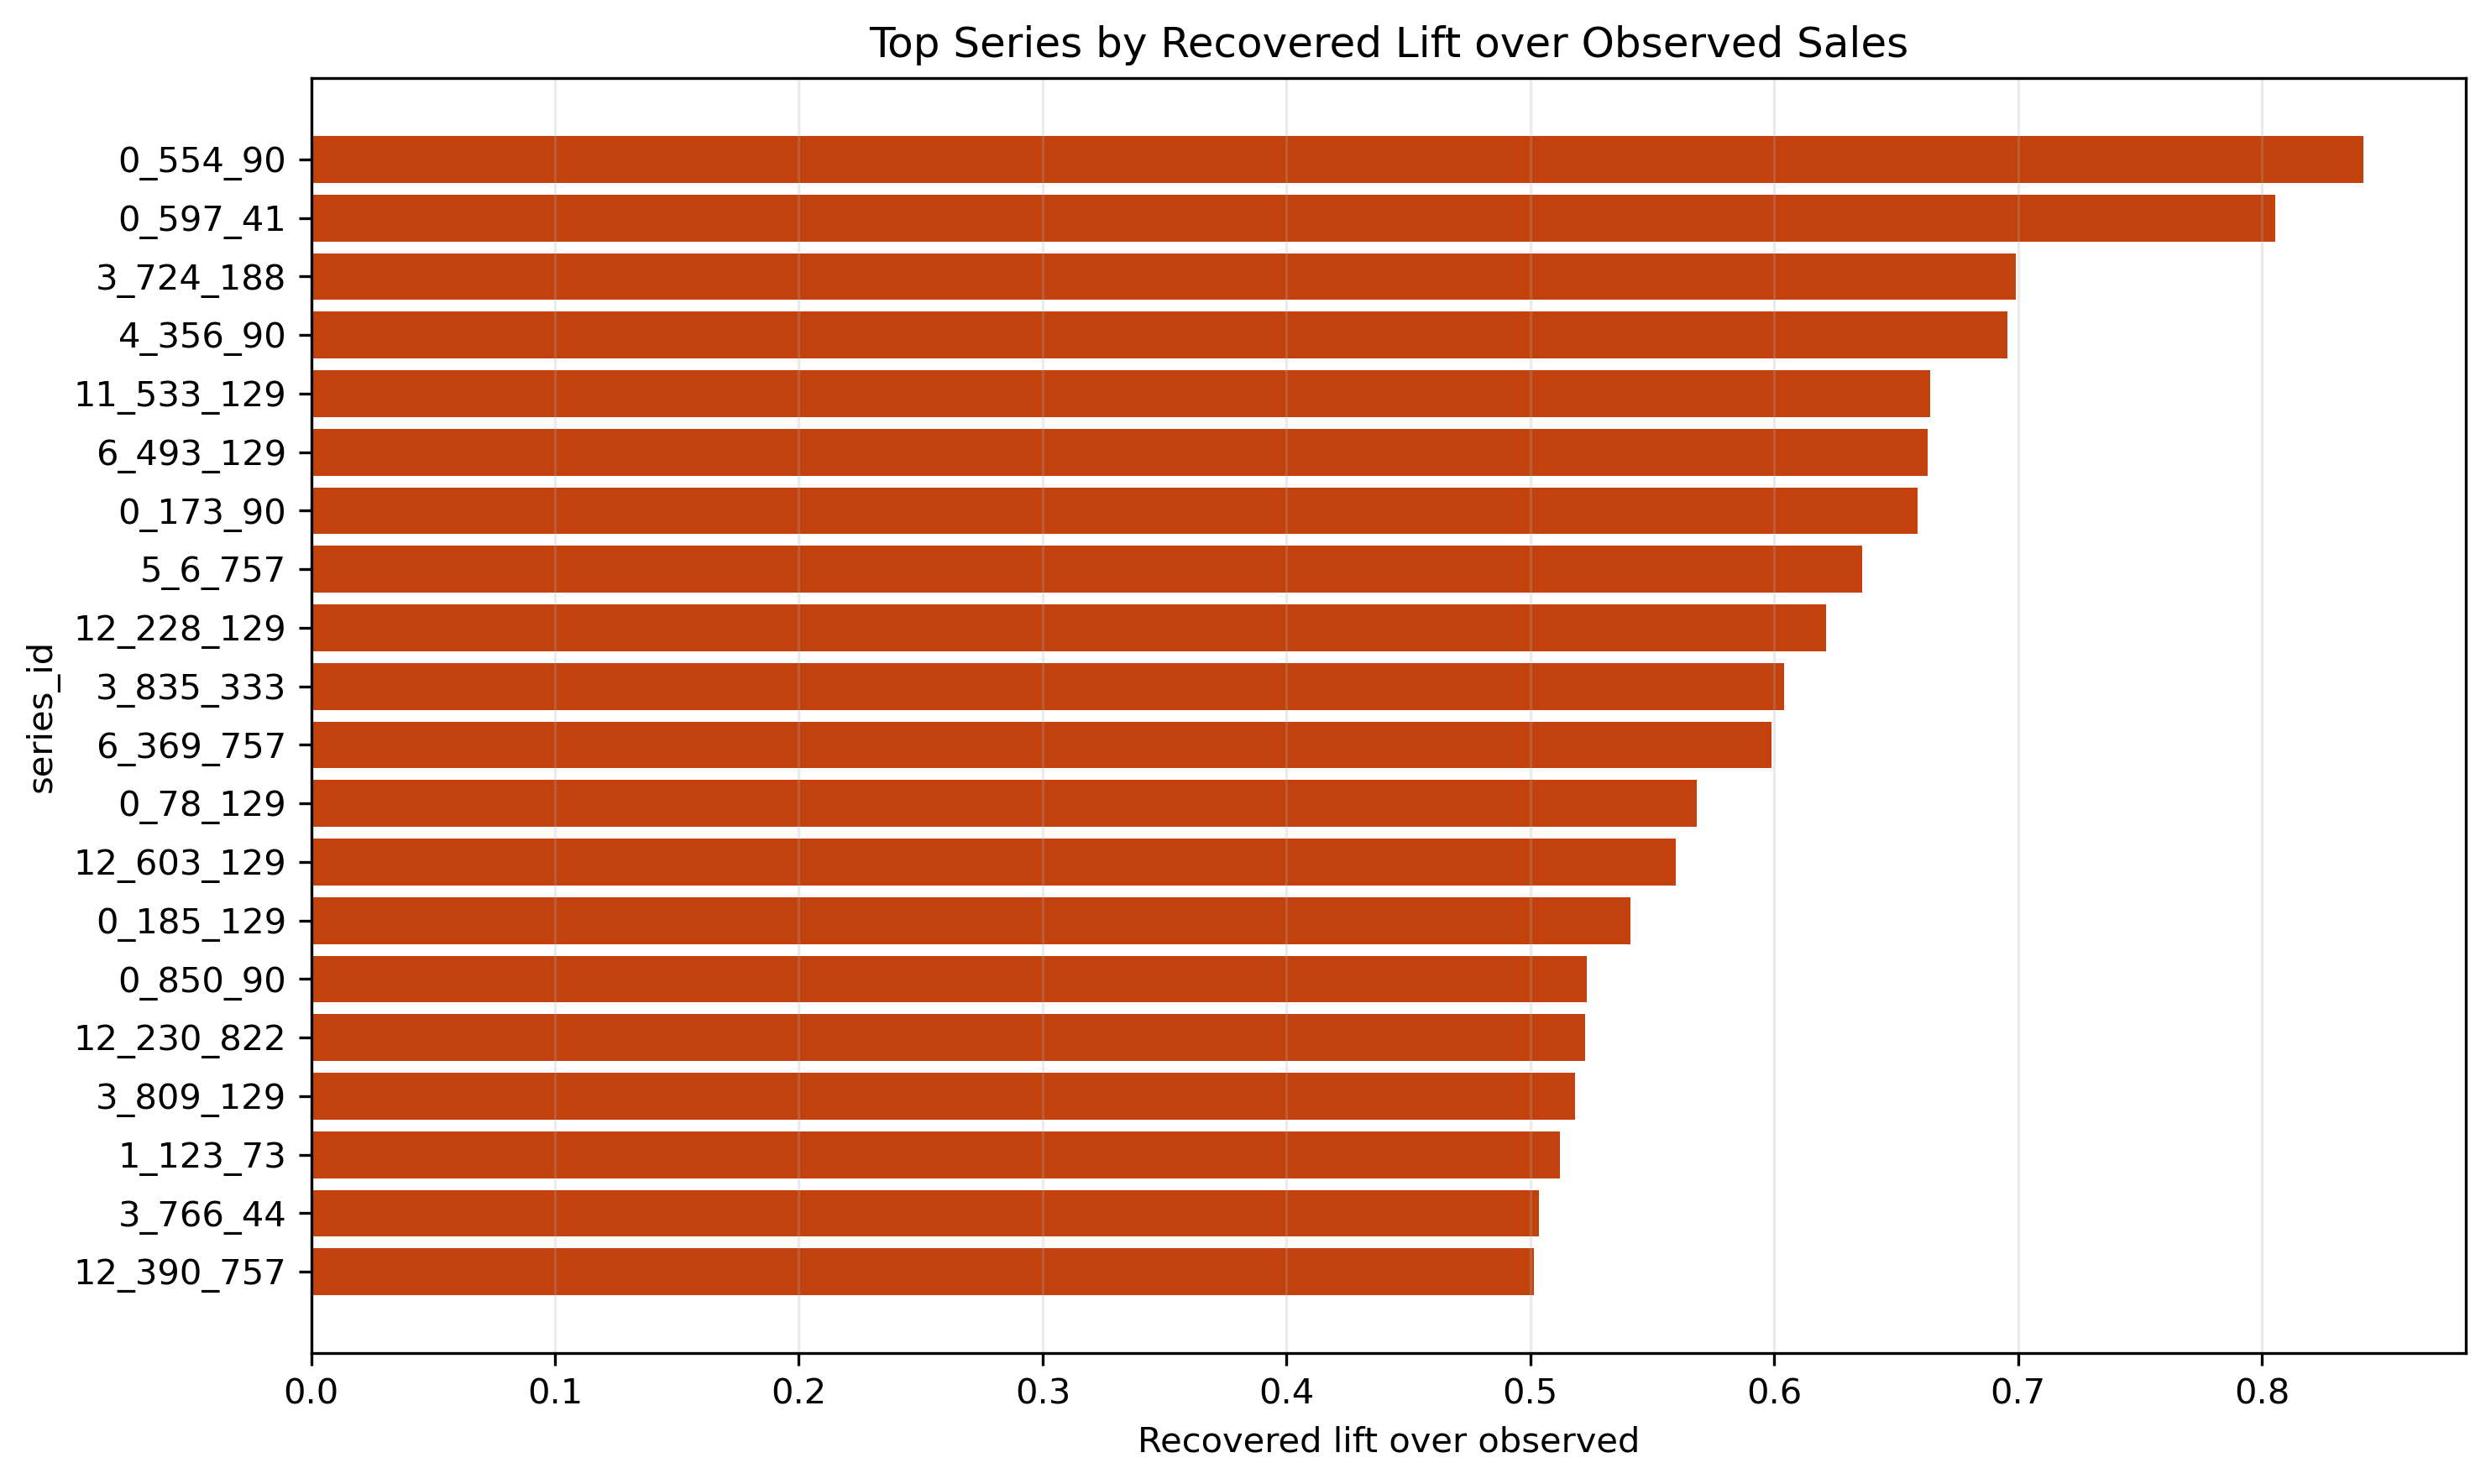
\includegraphics[width=0.78\linewidth]{figures/imputation_top_series_lift.png}
    \caption{Top series có lift cao nhất.}
    \label{fig:long-top-lift}
\end{figure}

\section{Forecasting results}

\subsection{So sánh không impute và có impute}

So sánh quan trọng nhất là giữa observed-sales forecasting và recovered-demand forecasting. Observed-sales LightGBM đại diện cho hướng không xử lý stockout trong target. Recovered-demand LightGBM đại diện cho hướng có recovery/imputation. Khi đánh giá trên recovered latent demand proxy, WAPE giảm từ 24.42\% xuống 20.28\%. Điều này cho thấy stockout-aware recovery giúp giảm under-forecast.


\begin{table}[H]
\centering
\caption{So sánh mô hình/baseline trên recovered latent demand proxy}
\label{tab:long-main-comparison}
\resizebox{\linewidth}{!}{%
\begin{tabular}{lllllllll}
\toprule
Model & Training target & Evaluation target & RMSE & MAE & WAPE & sMAPE & WPE & N \\
\midrule
Recovered naive x7 & baseline\_no\_training & Recovered latent demand proxy & 4.3949 & 2.8080 & 0.3149 & 0.3870 & -0.0198 & 70000 \\
Recovered seasonal naive 7-day & baseline\_no\_training & Recovered latent demand proxy & 2.9113 & 1.7704 & 0.1985 & 0.2269 & -0.0614 & 70000 \\
Recovered rolling mean 14-day & baseline\_no\_training & Recovered latent demand proxy & 3.1099 & 1.8367 & 0.2060 & 0.2268 & -0.0807 & 70000 \\
Observed-sales forecasting & target\_next7\_observed\_daily & Recovered latent demand proxy & 3.6749 & 2.1780 & 0.2442 & 0.2755 & -0.1788 & 70000 \\
Observed-sales forecasting & target\_next7\_observed\_daily & Observed sales & 3.2644 & 1.7730 & 0.2206 & 0.2412 & -0.0887 & 70000 \\
Recovered-demand forecasting & target\_next7\_recovered\_daily & Recovered latent demand proxy & 3.6160 & 1.8082 & 0.2028 & 0.2135 & -0.0800 & 70000 \\
Recovered-demand forecasting & target\_next7\_recovered\_daily & Observed sales & 3.4820 & 1.7713 & 0.2204 & 0.2459 & 0.0209 & 70000 \\
Recovered seasonal-ML hybrid & seasonal\_naive\_plus\_recovered\_lightgbm\_alpha\_0.60 & Recovered latent demand proxy & 3.2106 & 1.7545 & 0.1967 & 0.2127 & -0.0726 & 70000 \\
\bottomrule
\end{tabular}
}
\end{table}



\begin{figure}[H]
    \centering
    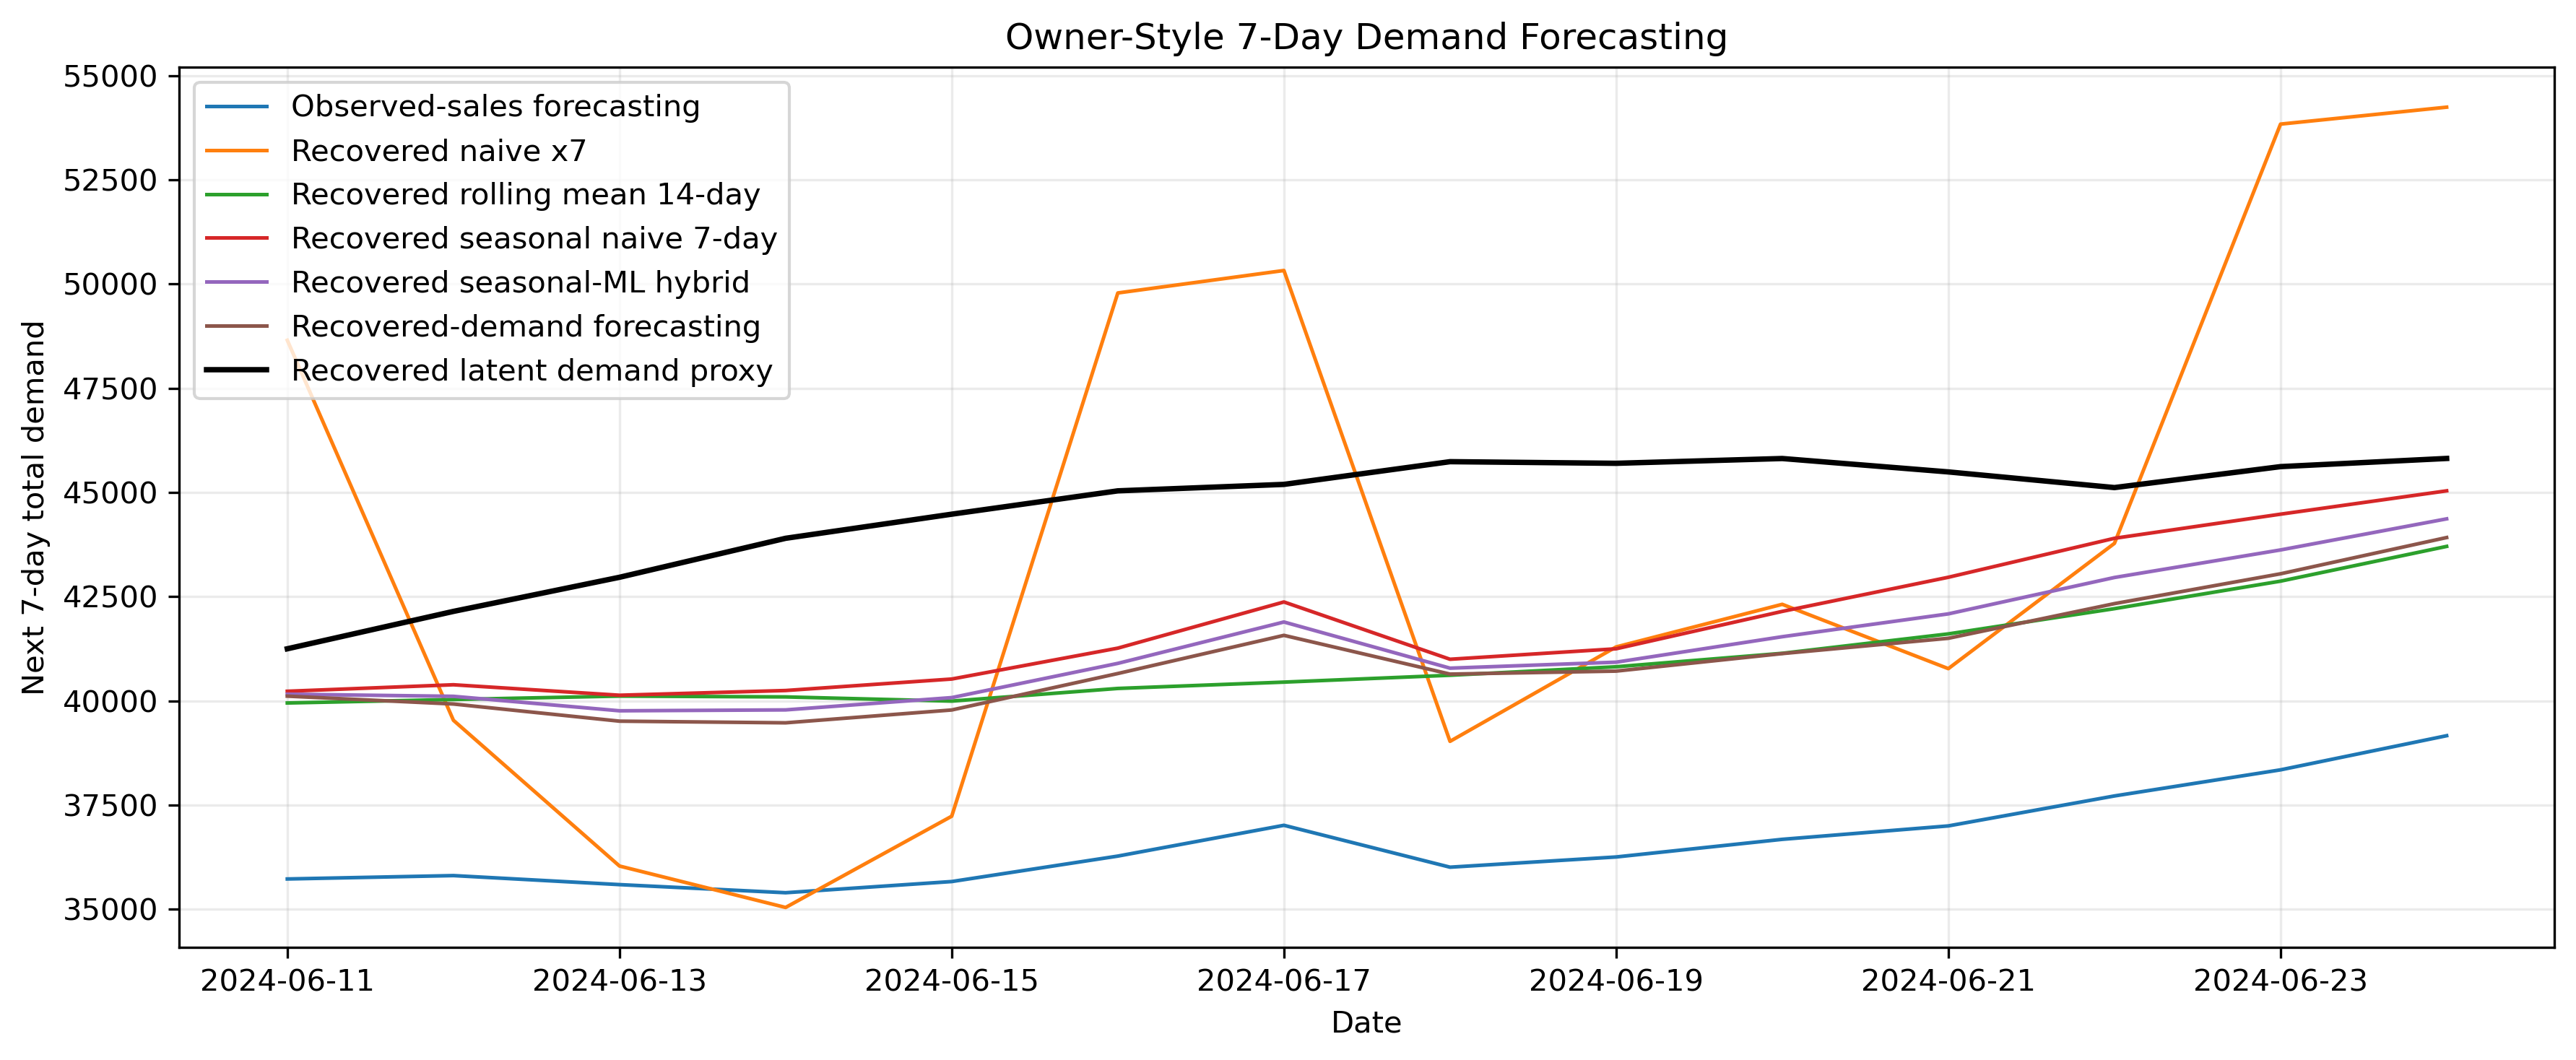
\includegraphics[width=0.92\linewidth]{figures/owner_two_stage_forecast_comparison.png}
    \caption{Forecast tổng nhu cầu 7 ngày.}
    \label{fig:long-forecast-comparison}
\end{figure}



\begin{figure}[H]
    \centering
    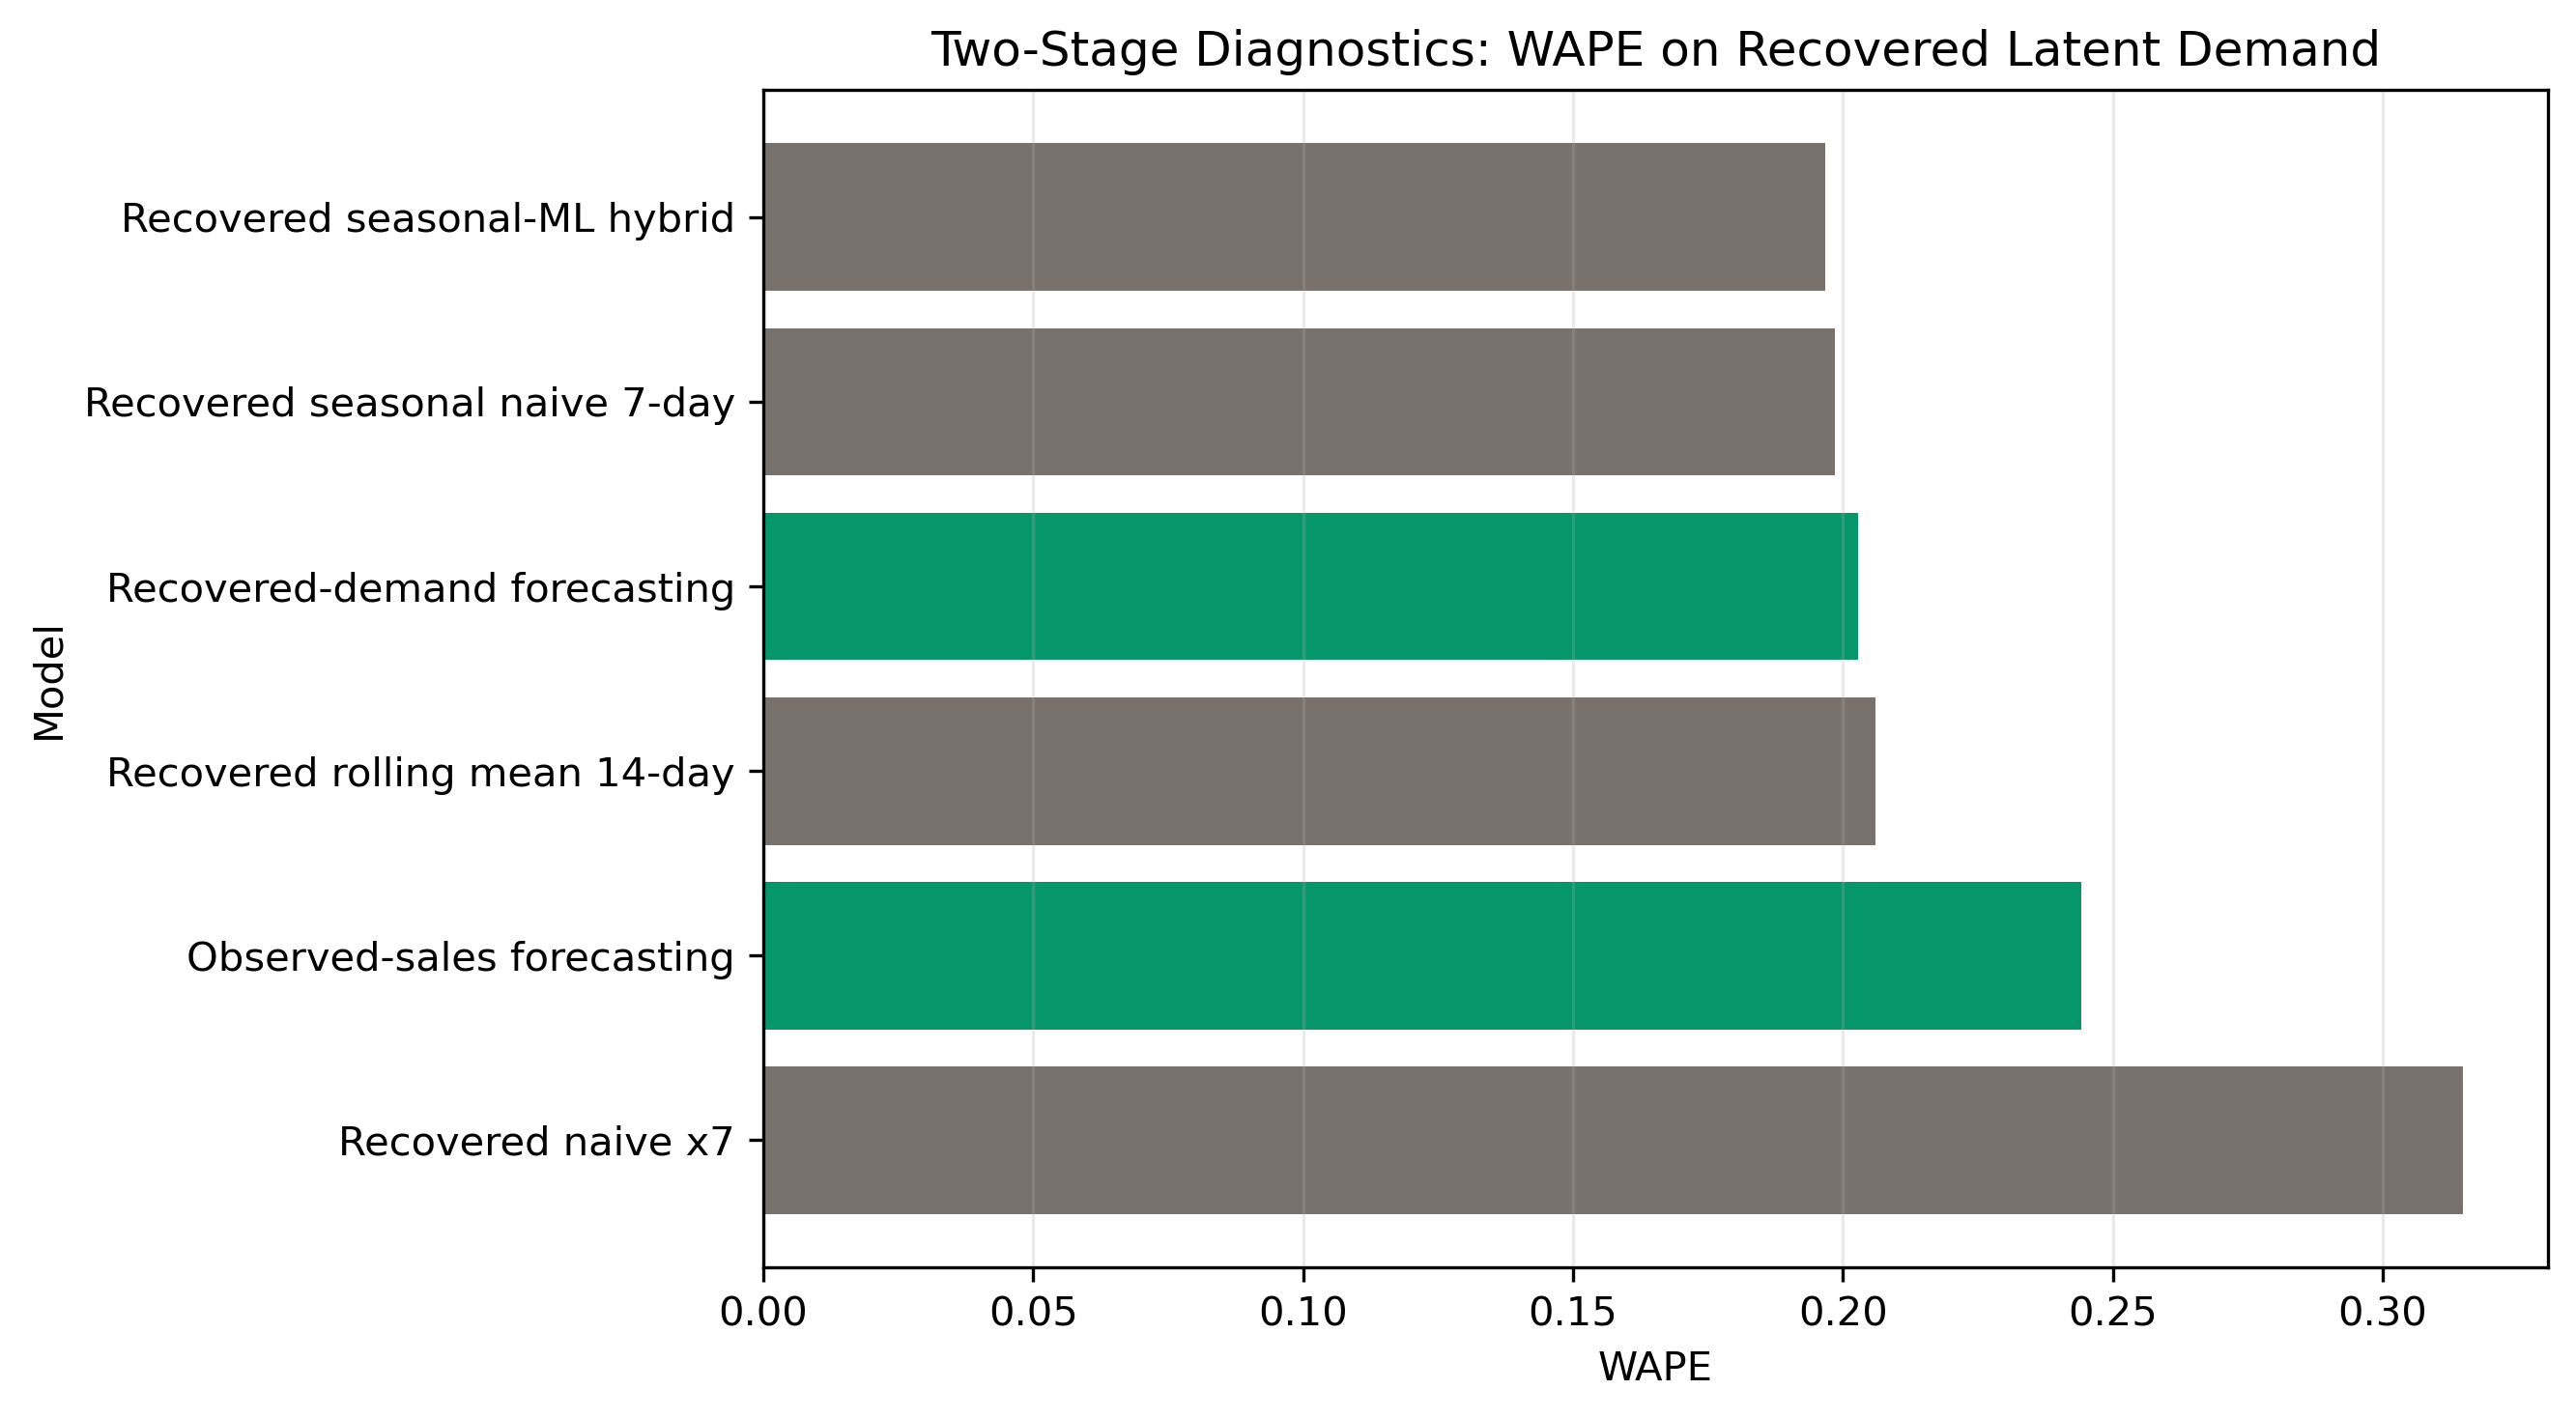
\includegraphics[width=0.92\linewidth]{figures/owner_two_stage_diagnostics_wape.png}
    \caption{WAPE của các mô hình/baseline trên recovered latent demand proxy.}
    \label{fig:long-wape}
\end{figure}


\subsection{Seasonal naive là baseline mạnh}

Seasonal naive 7-day đạt WAPE 19.85\%, tốt hơn recovered-demand LightGBM thuần. Đây không phải thất bại của ML mà là insight quan trọng: pattern tuần là thành phần nền rất mạnh. Một mô hình tốt trong bài toán này cần tôn trọng seasonality thay vì cố học lại hoàn toàn từ đầu.

\subsection{Hybrid seasonal-ML}

Hybrid seasonal-ML blend seasonal naive 7-day với recovered-demand LightGBM. Trọng số LightGBM được chọn trên validation set, không chọn bằng test. Trọng số tốt nhất hiện tại là 0.60 cho LightGBM và 0.40 cho seasonal naive. Kết quả test đạt WAPE 19.67\%, tốt nhất trong nhóm đã thử.


\begin{table}[H]
\centering
\caption{Chọn trọng số hybrid trên validation}
\label{tab:long-hybrid-blend}
\resizebox{0.80\linewidth}{!}{%
\begin{tabular}{lll}
\toprule
LightGBM weight & Seasonal naive weight & Validation WAPE \\
\midrule
0.6000 & 0.4000 & 0.1901 \\
0.5500 & 0.4500 & 0.1901 \\
0.6500 & 0.3500 & 0.1902 \\
0.5000 & 0.5000 & 0.1903 \\
0.7000 & 0.3000 & 0.1903 \\
0.4500 & 0.5500 & 0.1906 \\
0.7500 & 0.2500 & 0.1906 \\
0.4000 & 0.6000 & 0.1909 \\
0.8000 & 0.2000 & 0.1909 \\
0.3500 & 0.6500 & 0.1914 \\
\bottomrule
\end{tabular}
}
\end{table}


\subsection{Business interpretation}

Ý nghĩa của kết quả không chỉ là giảm WAPE. Nếu doanh nghiệp forecast observed sales, model có thể tiếp tục đánh giá thấp nhu cầu ở các SKU hay hết hàng. Recovery làm rõ phần demand bị ẩn, còn seasonal baseline cho thấy lịch tuần là thông tin vận hành rất quan trọng. Hybrid cuối cùng kết hợp cả hai: demand correction và weekly seasonality.

\subsection{Feature importance}

Feature importance của recovered-demand LightGBM cho thấy các lag và rolling features của recovered demand, cùng với stockout rate, là các tín hiệu quan trọng. Điều này phù hợp với trực giác: demand tương lai phụ thuộc mạnh vào mức nền gần đây, pattern tuần và mức độ kiểm duyệt bởi tồn kho.


\begin{table}[H]
\centering
\caption{Feature importance của recovered-demand LightGBM}
\label{tab:long-feature-importance}
\resizebox{0.75\linewidth}{!}{%
\begin{tabular}{ll}
\toprule
feature & importance \\
\midrule
stockout\_rate & 986 \\
recovered\_daily\_lag\_28 & 969 \\
recovered\_daily\_lag\_1 & 820 \\
recovered\_daily\_lag\_14 & 814 \\
recovered\_daily\_lag\_7 & 794 \\
recovered\_daily\_lag\_2 & 699 \\
recovered\_daily\_roll\_mean\_28 & 671 \\
recovered\_daily\_roll\_sum\_28 & 585 \\
day\_of\_week & 518 \\
recovered\_daily\_roll\_mean\_7 & 490 \\
month & 410 \\
recovered\_daily\_roll\_mean\_14 & 392 \\
recovered\_daily\_roll\_sum\_14 & 329 \\
recovered\_daily\_roll\_sum\_7 & 289 \\
is\_weekend & 23 \\
\bottomrule
\end{tabular}
}
\end{table}



\begin{figure}[H]
    \centering
    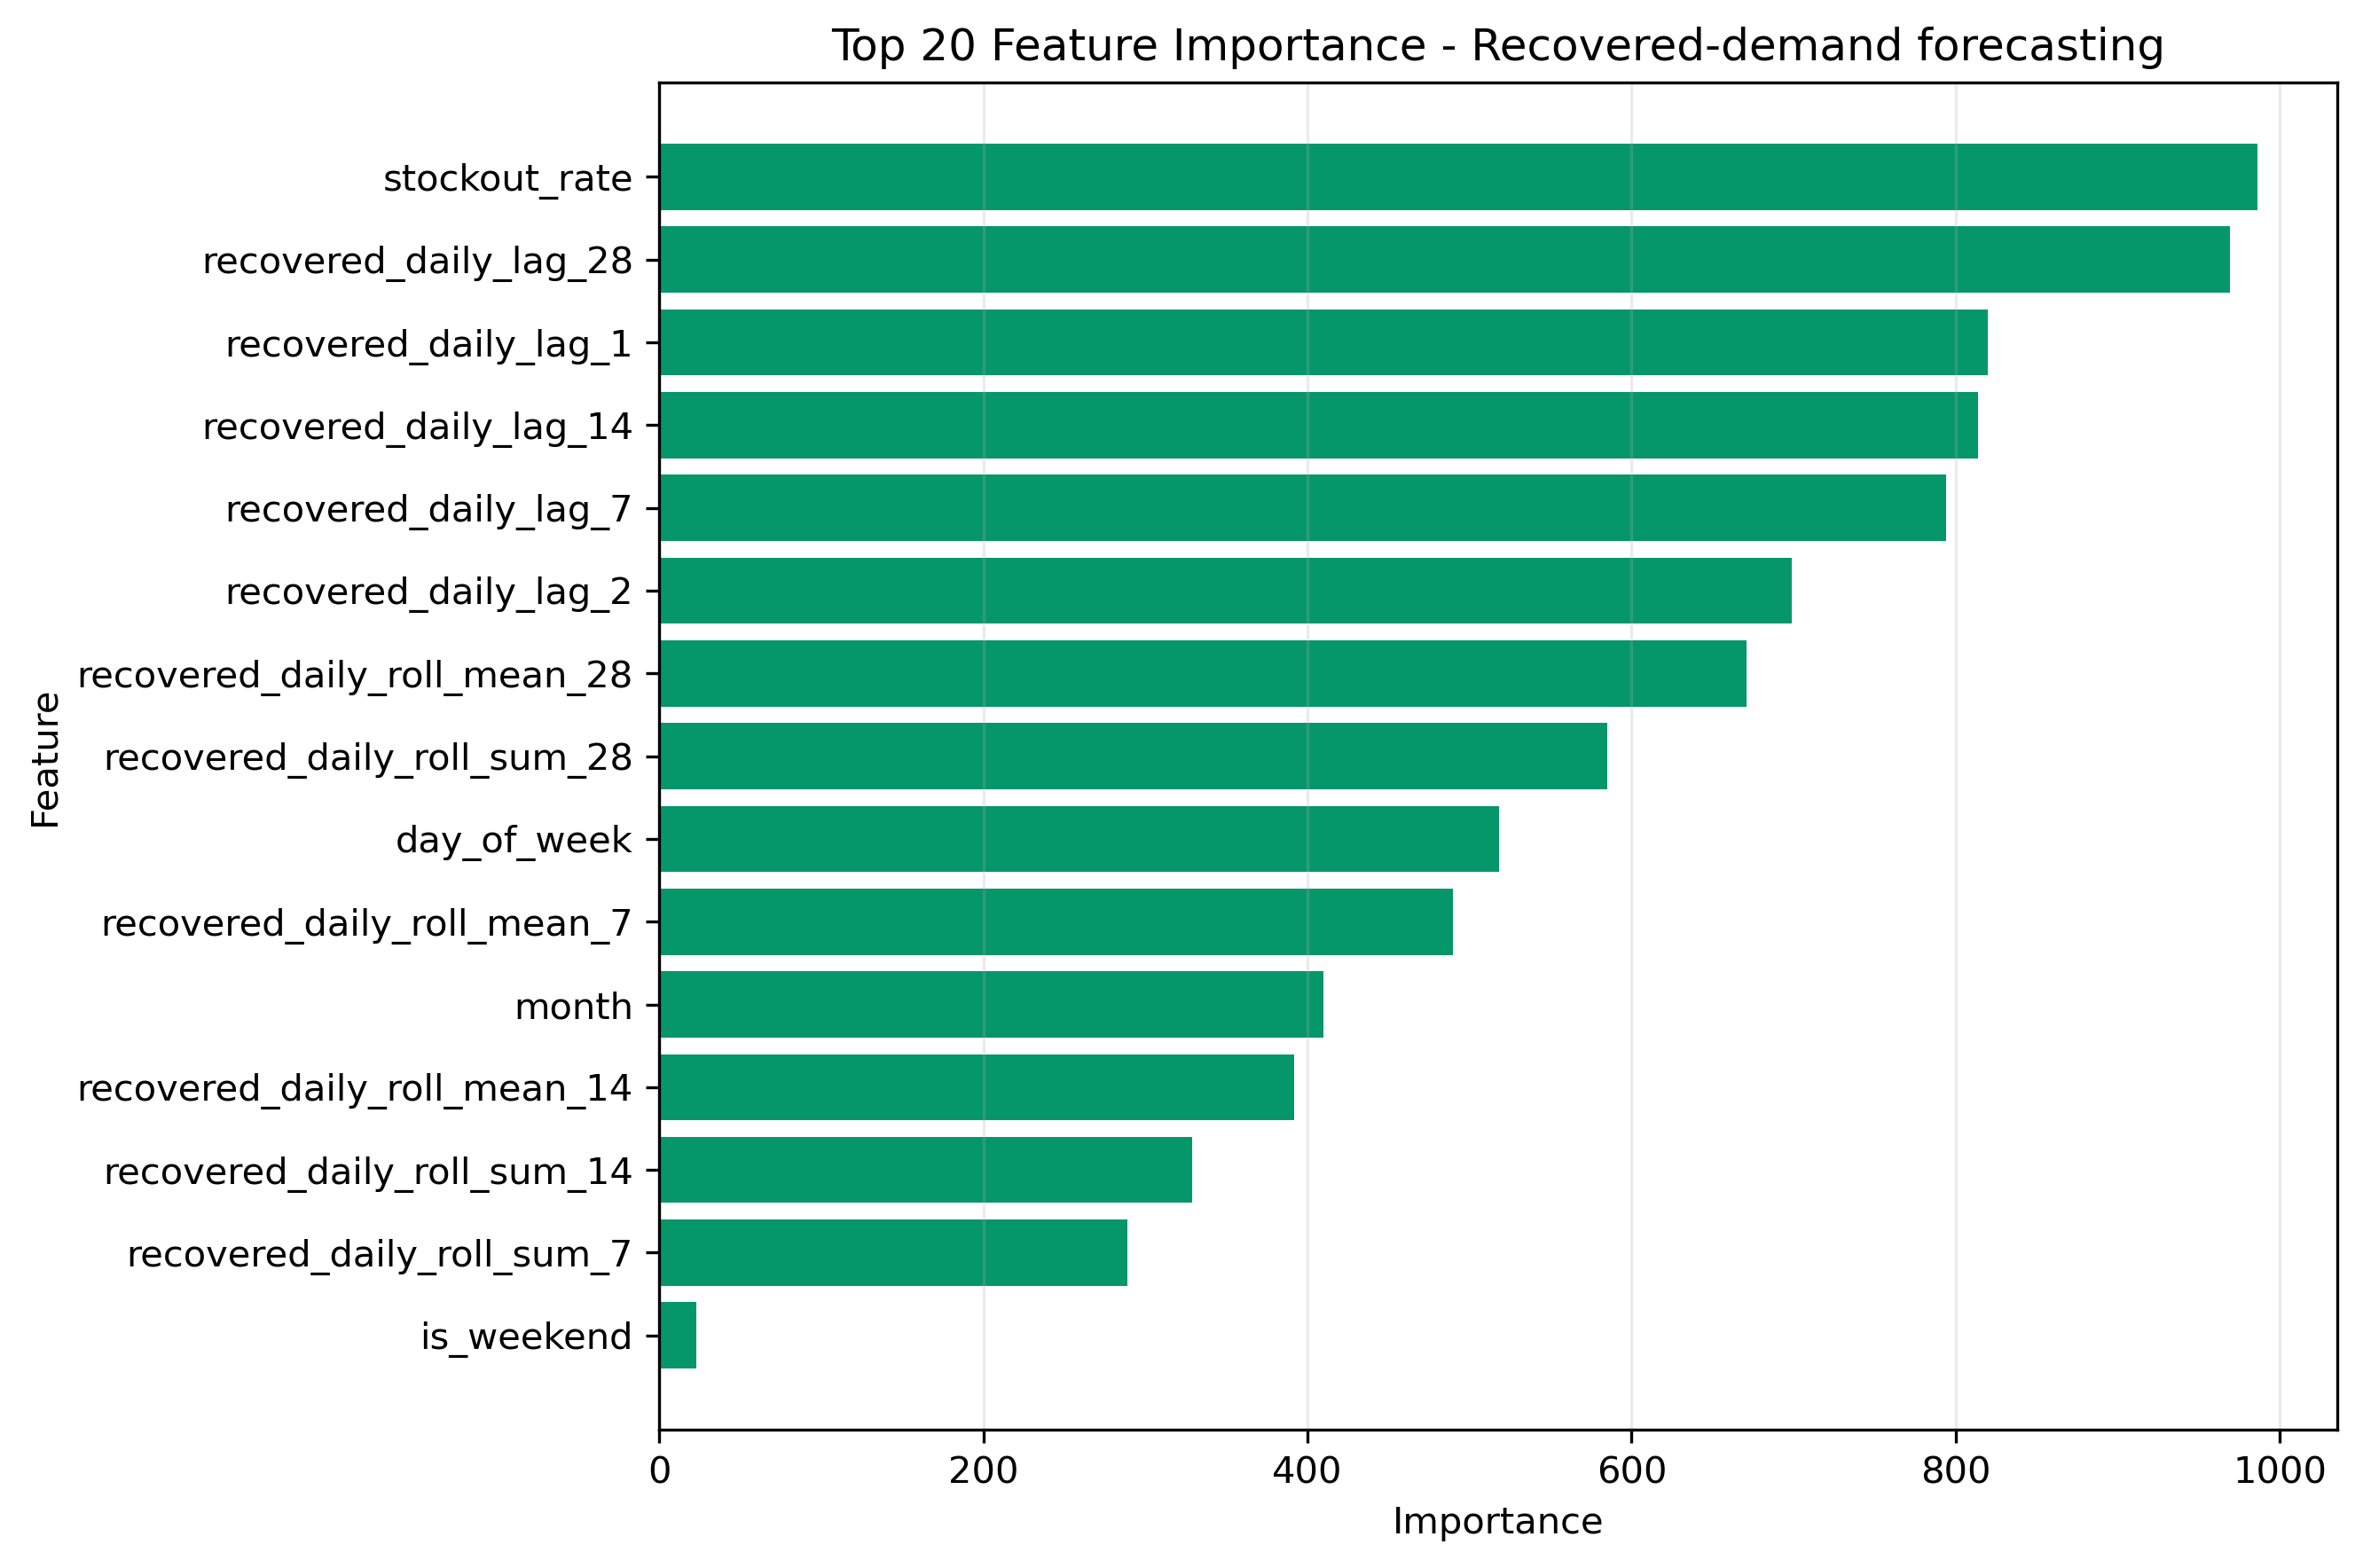
\includegraphics[width=0.78\linewidth]{figures/owner_recovereddemand_forecasting_feature_importance_top20.png}
    \caption{Top 20 feature importance.}
    \label{fig:long-feature-importance}
\end{figure}

\section{Diagnostics và forecast uncertainty}

\subsection{Residual diagnostics}

Diagnostics được thực hiện trên recovered latent demand proxy. Với target là tổng 7 ngày tiếp theo, các forecast origin liên tiếp có target window overlap mạnh: forecast tại ngày $t$ và ngày $t+1$ chia sẻ 6/7 ngày trong target. Vì vậy, residual rolling evaluation có thể còn autocorrelation một phần do thiết kế target, không nhất thiết chỉ do model thiếu pattern.


\begin{table}[H]
\centering
\caption{Diagnostics trên recovered latent demand proxy}
\label{tab:long-diagnostics}
\resizebox{\linewidth}{!}{%
\begin{tabular}{llllllllll}
\toprule
Model & RMSE & MAE & WAPE & WPE & Residual mean & Residual std & Ljung-Box p-value & Jarque-Bera p-value & N \\
\midrule
Recovered naive x7 & 4.3949 & 2.8080 & 0.3149 & -0.0198 & 0.1770 & 4.3913 & 0.1790 & 0.0000 & 70000 \\
Recovered seasonal naive 7-day & 2.9113 & 1.7704 & 0.1985 & -0.0614 & 0.5475 & 2.8594 & 0.0131 & 0.0000 & 70000 \\
Recovered rolling mean 14-day & 3.1099 & 1.8367 & 0.2060 & -0.0807 & 0.7194 & 3.0255 & 0.0001 & 0.0000 & 70000 \\
Observed-sales forecasting & 3.6749 & 2.1780 & 0.2442 & -0.1788 & 1.5943 & 3.3111 & 0.0127 & 0.0000 & 70000 \\
Recovered-demand forecasting & 3.6160 & 1.8082 & 0.2028 & -0.0800 & 0.7134 & 3.5450 & 0.0665 & 0.0000 & 70000 \\
Recovered seasonal-ML hybrid & 3.2106 & 1.7545 & 0.1967 & -0.0726 & 0.6470 & 3.1448 & 0.0311 & 0.0000 & 70000 \\
\bottomrule
\end{tabular}
}
\end{table}



\begin{figure}[H]
    \centering
    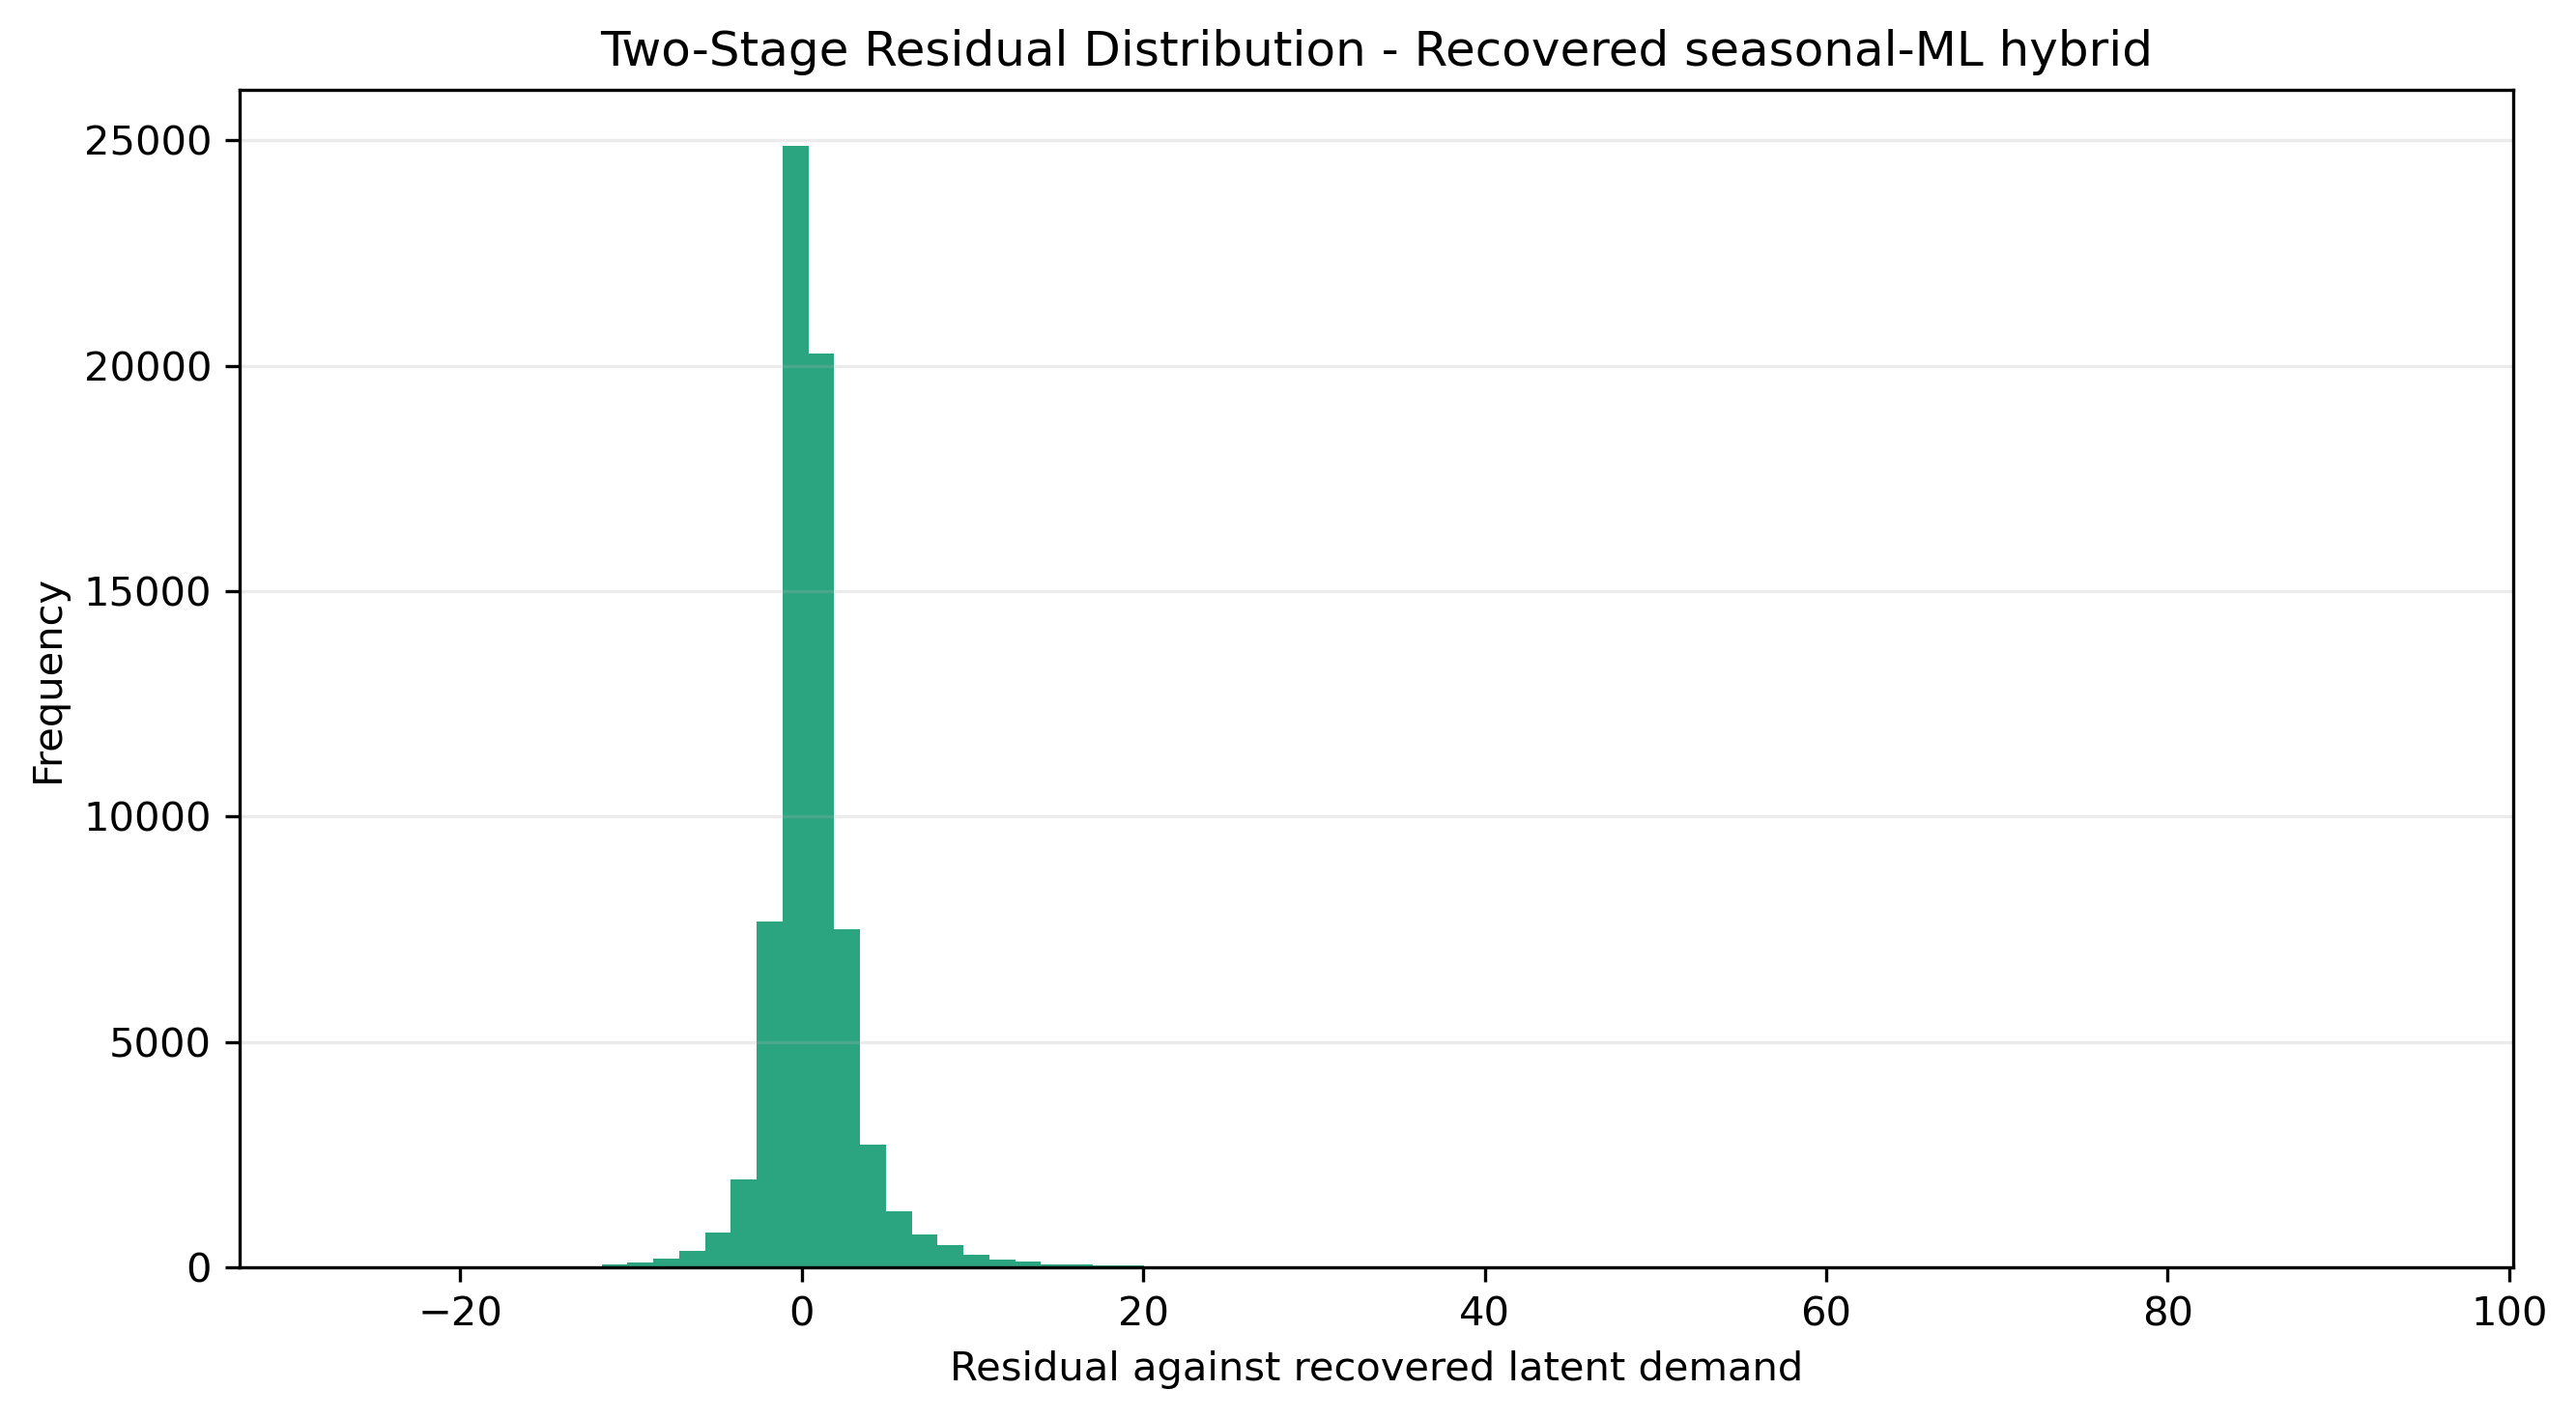
\includegraphics[width=0.78\linewidth]{figures/owner_two_stage_residual_distribution.png}
    \caption{Phân phối residual của mô hình chính.}
    \label{fig:long-residual-dist}
\end{figure}



\begin{figure}[H]
    \centering
    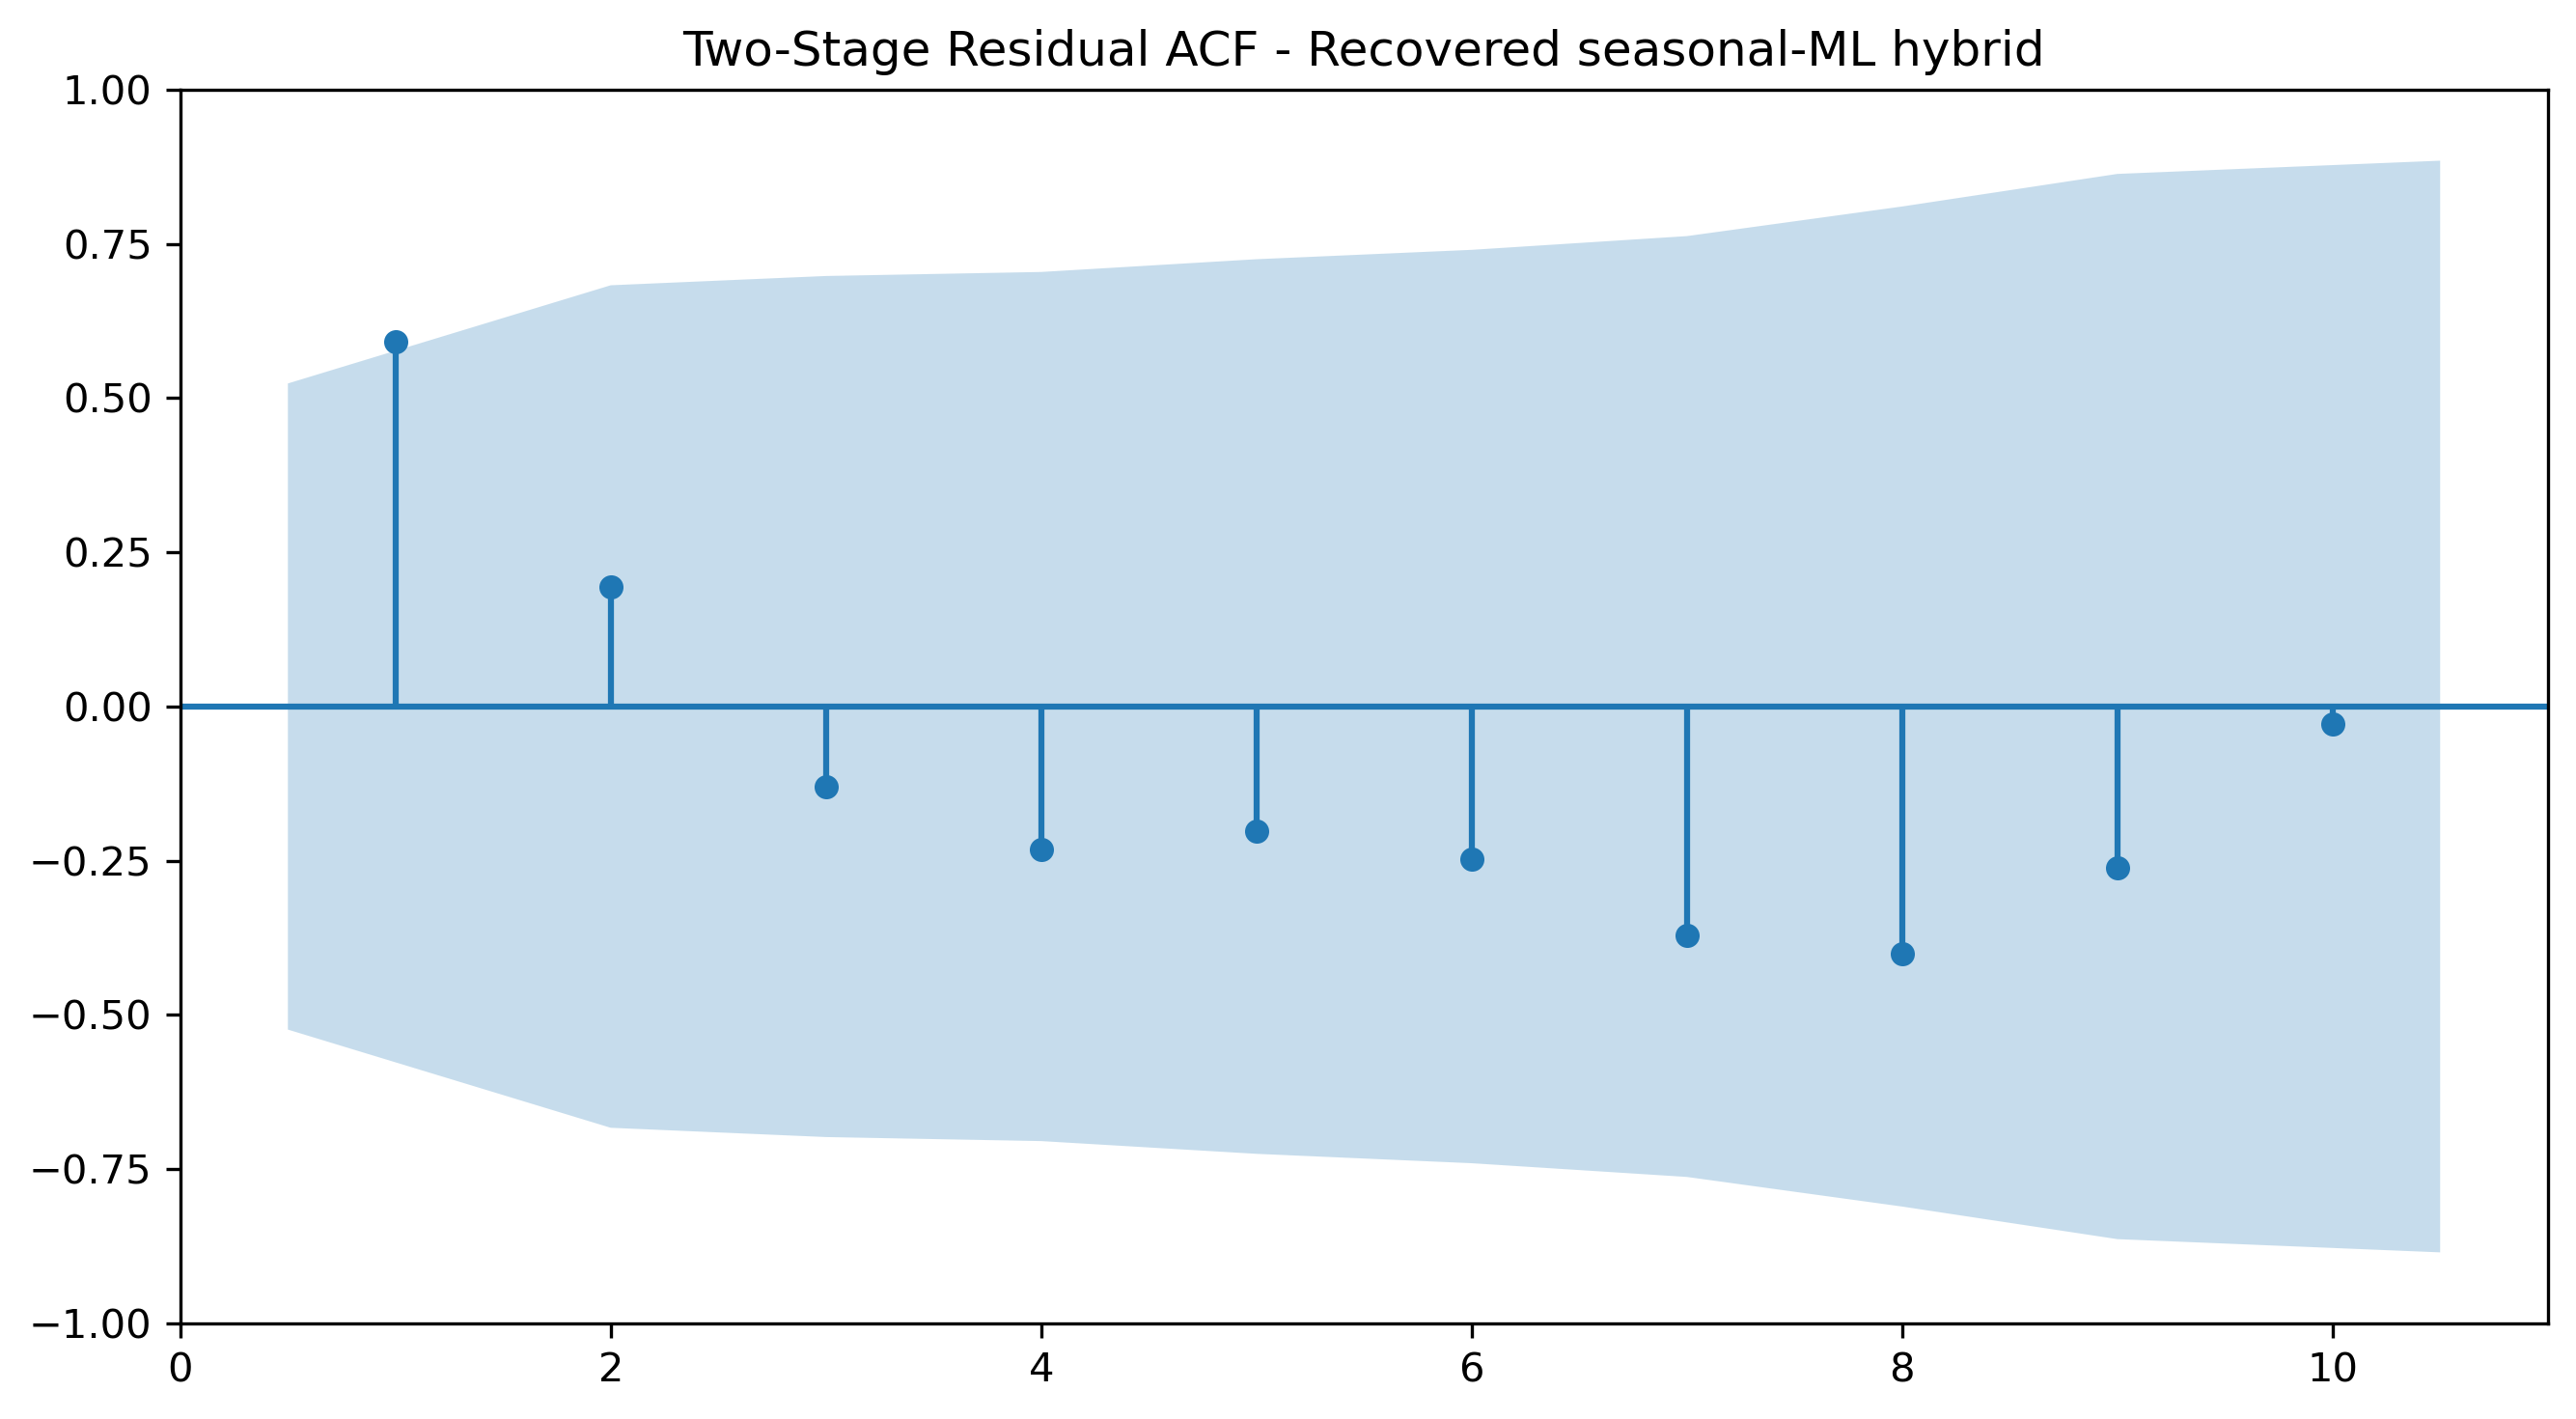
\includegraphics[width=0.82\linewidth]{figures/owner_two_stage_residual_acf.png}
    \caption{Residual ACF của mô hình chính.}
    \label{fig:long-residual-acf}
\end{figure}


\subsection{Non-overlap diagnostics}

Báo cáo bổ sung non-overlap diagnostics bằng cách lấy forecast origin cách nhau 7 ngày. Kiểm tra này công bằng hơn với target next-7-day, nhưng test window chỉ có 14 ngày nên chỉ có rất ít aggregate points. Vì vậy, đây là sanity check phụ, không phải bằng chứng tuyệt đối rằng residual độc lập hoàn toàn.


\begin{table}[H]
\centering
\caption{Diagnostics trên non-overlapping 7-day targets}
\label{tab:long-nonoverlap}
\resizebox{\linewidth}{!}{%
\begin{tabular}{lllllllll}
\toprule
Model & Evaluation dates & RMSE & MAE & WAPE & WPE & Ljung-Box p-value & N & Aggregate residual points \\
\midrule
Recovered naive x7 & 2024-06-11; 2024-06-18 & 4.6707 & 2.9483 & 0.3389 & 0.0080 & 0.1573 & 10000 & 2 \\
Recovered seasonal naive 7-day & 2024-06-11; 2024-06-18 & 2.8150 & 1.7140 & 0.1970 & -0.0662 & 0.1573 & 10000 & 2 \\
Recovered rolling mean 14-day & 2024-06-11; 2024-06-18 & 3.0150 & 1.7821 & 0.2049 & -0.0738 & 0.1573 & 10000 & 2 \\
Observed-sales forecasting & 2024-06-11; 2024-06-18 & 3.5320 & 2.1044 & 0.2419 & -0.1753 & 0.1573 & 10000 & 2 \\
Recovered-demand forecasting & 2024-06-11; 2024-06-18 & 3.3906 & 1.7544 & 0.2017 & -0.0716 & 0.1573 & 10000 & 2 \\
Recovered seasonal-ML hybrid & 2024-06-11; 2024-06-18 & 3.0564 & 1.7001 & 0.1954 & -0.0695 & 0.1573 & 10000 & 2 \\
\bottomrule
\end{tabular}
}
\end{table}


\subsection{Prediction intervals}

Khoảng dự báo được xây dựng từ phân vị residual validation. Cách này không giả định residual chuẩn tuyệt đối, phù hợp hơn với dữ liệu bán lẻ thưa và nhiều spike.


\begin{figure}[H]
    \centering
    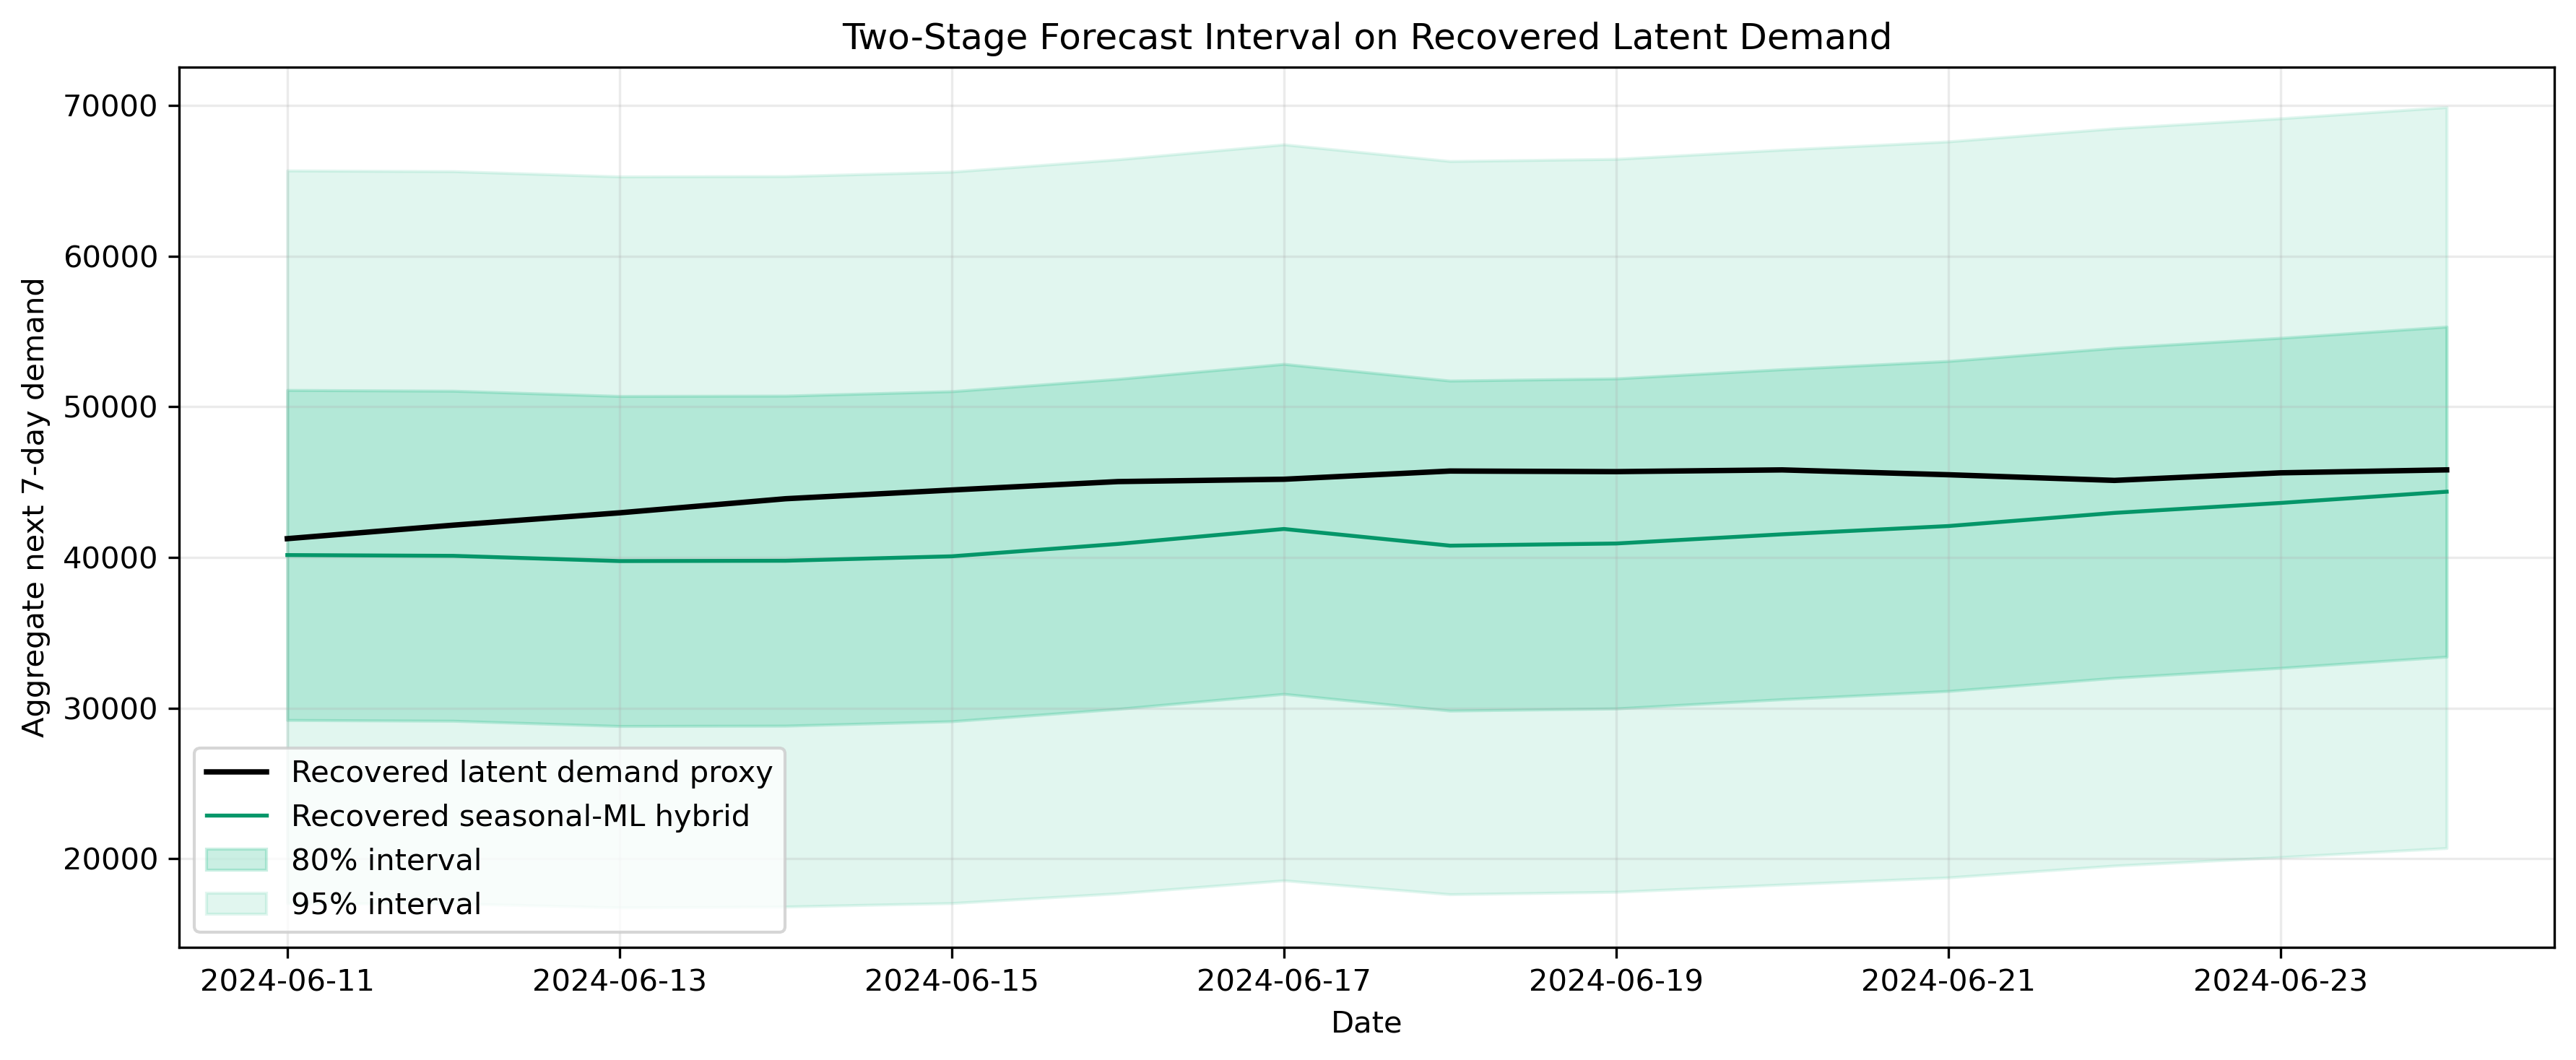
\includegraphics[width=0.92\linewidth]{figures/owner_two_stage_forecast_interval.png}
    \caption{Khoảng dự báo 80\textbackslash\{\}\% và 95\textbackslash\{\}\% cho mô hình chính.}
    \label{fig:long-forecast-interval}
\end{figure}

\section{Business insights}

\subsection{Insight 1: Stockout làm sai lệch tín hiệu demand}

Tỷ lệ stockout row khoảng 24.65\% cho thấy đây không phải hiện tượng hiếm. Nếu doanh nghiệp chỉ quan sát sales, một phần demand bị ẩn sẽ bị hiểu nhầm là demand thấp. Trong vận hành tồn kho, đây là vấn đề nghiêm trọng vì forecast thấp dẫn tới reorder thấp.

\subsection{Insight 2: Latent demand recovery cho biết mức demand bị bỏ lỡ}

Recovered demand tăng khoảng 10.68\% so với observed sales. Con số này không nên hiểu là doanh nghiệp chắc chắn mất đúng từng đó doanh số, vì recovered demand là proxy. Tuy nhiên, nó là chỉ báo hữu ích: observed sales có khả năng đang understated demand ở mức đáng kể.

\subsection{Insight 3: Weekly seasonality là baseline nghiệp vụ mạnh}

Seasonal naive 7-day rất mạnh. Về business, điều này nghĩa là nhu cầu trong bán lẻ có lịch tuần rõ ràng. Khi triển khai hệ thống forecast, không nên bỏ qua các quy tắc đơn giản như lấy demand cùng kỳ tuần trước. ML chỉ có ý nghĩa khi nó cải thiện trên nền seasonality mạnh đó hoặc kết hợp tốt với nó.

\subsection{Insight 4: Model cuối nên hỗ trợ replenishment}

Mục tiêu cuối không phải tạo model có metric đẹp nhất trong phòng thí nghiệm, mà là hỗ trợ quyết định nhập hàng. Forecast recovered demand phù hợp hơn observed sales vì nó hướng tới nhu cầu vận hành. Hybrid seasonal-ML có thể xem là một forecast thực dụng: dùng seasonality làm nền, dùng ML để hiệu chỉnh theo stockout và pattern gần đây.

\subsection{Khuyến nghị triển khai}

Nếu triển khai thực tế, hệ thống nên báo cáo song song observed sales forecast và recovered demand forecast. Khi hai giá trị lệch nhau lớn ở các SKU có stockout cao, đây là tín hiệu cần kiểm tra replenishment. Doanh nghiệp cũng nên theo dõi uplift do imputation theo SKU/store để phát hiện nhóm sản phẩm có rủi ro mất doanh số do hết hàng.

\section{Kết luận, hạn chế và hướng phát triển}

\subsection{Kết luận}

Báo cáo cho thấy bài toán forecasting trên FreshRetailNet-50K nên được framing như bài toán stockout-aware demand forecasting thay vì raw sales forecasting. Khi không xử lý stockout, observed-sales LightGBM đạt WAPE 24.42\%. Sau khi recover latent demand và train trên recovered demand, WAPE giảm xuống 20.28\%. Seasonal naive 7-day là baseline mạnh với WAPE 19.85\%. Mô hình cuối hybrid seasonal-ML đạt WAPE 19.67\%.

Kết quả này có hai thông điệp chính. Thứ nhất, xử lý stockout là cần thiết vì observed sales có thể understates demand. Thứ hai, seasonality tuần là pattern nền cực mạnh; một mô hình forecasting tốt nên kết hợp seasonality này thay vì bỏ qua.

\subsection{Hạn chế}

Recovered demand vẫn là proxy được ước lượng, không phải ground truth demand thật. Imputation ở cấp hourly row-level nhiễu vì dữ liệu thưa và nhiều zero. Test window chỉ kéo dài 14 ngày nên diagnostics non-overlap còn ít điểm. Ngoài ra, báo cáo chưa trực tiếp tối ưu inventory policy như safety stock, reorder point, service level hoặc lost-sales cost.

\subsection{Hướng phát triển}

Nếu có thêm thời gian, hướng phát triển đầu tiên là kiểm tra pipeline trên nhiều sample hoặc full data. Hướng thứ hai là thử các mô hình imputation chuyên biệt như SAITS, TimesNet hoặc DLinear ở quy mô nhỏ để so sánh với LightGBM recovery. Hướng thứ ba là chuyển từ forecast accuracy sang inventory impact: service level, fill rate, lost sales và holding cost. Đây là bước quan trọng để biến forecast thành quyết định vận hành.

\appendix
\section{Phụ lục A: Bảng hỗ trợ trực tiếp}

Phụ lục chỉ giữ các bảng hỗ trợ trực tiếp cho contribution chính: recovery không leakage, kiểm soát imputation, diagnostics phụ và khả năng tái lập. Các benchmark observed-sales hourly, ablation cũ, SARIMAX aggregate và các bảng thử nghiệm phụ được giữ trong thư mục \texttt{archive\_auxiliary/} thay vì đưa vào báo cáo chính, để tránh làm loãng câu chuyện.


\begin{table}[H]
\centering
\caption{Các block expanding-window dùng cho recovery}
\label{tab:app-recovery-blocks}
\resizebox{\linewidth}{!}{%
\begin{tabular}{lllll}
\toprule
Block start & Block end & Training end & Training rows & Predicted rows \\
\midrule
2024-04-11 & 2024-04-18 & 2024-04-10 23:00:00 & 400000 & 840000 \\
2024-04-18 & 2024-04-25 & 2024-04-17 23:00:00 & 400000 & 840000 \\
2024-04-25 & 2024-05-02 & 2024-04-24 23:00:00 & 400000 & 840000 \\
2024-05-02 & 2024-05-09 & 2024-05-01 23:00:00 & 400000 & 840000 \\
2024-05-09 & 2024-05-16 & 2024-05-08 23:00:00 & 400000 & 840000 \\
2024-05-16 & 2024-05-23 & 2024-05-15 23:00:00 & 400000 & 840000 \\
2024-05-23 & 2024-05-30 & 2024-05-22 23:00:00 & 400000 & 840000 \\
2024-05-30 & 2024-06-06 & 2024-05-29 23:00:00 & 400000 & 840000 \\
2024-06-06 & 2024-06-11 & 2024-06-05 23:00:00 & 400000 & 600000 \\
\bottomrule
\end{tabular}
}
\end{table}



\begin{table}[H]
\centering
\caption{Top series theo recovered lift}
\label{tab:app-series-uplift}
\resizebox{\linewidth}{!}{%
\begin{tabular}{lllllll}
\toprule
series\_id & observed\_sales & recovered\_demand & recovered\_lost\_demand & stockout\_rate & Recovered lift over observed & Recovered share from imputation \\
\midrule
0\_554\_90 & 39.3000 & 72.3776 & 33.0776 & 0.7339 & 0.8417 & 0.4570 \\
0\_597\_41 & 39.8500 & 71.9541 & 32.1041 & 0.6150 & 0.8056 & 0.4462 \\
3\_724\_188 & 45.3000 & 76.9671 & 31.6671 & 0.7248 & 0.6991 & 0.4114 \\
4\_356\_90 & 39.0500 & 66.2217 & 27.1717 & 0.6029 & 0.6958 & 0.4103 \\
11\_533\_129 & 43.7000 & 72.7158 & 29.0158 & 0.7161 & 0.6640 & 0.3990 \\
6\_493\_129 & 44.2000 & 73.4980 & 29.2980 & 0.7357 & 0.6629 & 0.3986 \\
0\_173\_90 & 55.3000 & 91.7408 & 36.4408 & 0.6536 & 0.6590 & 0.3972 \\
5\_6\_757 & 44.5000 & 72.8119 & 28.3119 & 0.7448 & 0.6362 & 0.3888 \\
12\_228\_129 & 45.7000 & 74.0857 & 28.3857 & 0.6667 & 0.6211 & 0.3831 \\
3\_835\_333 & 46.7000 & 74.9063 & 28.2063 & 0.6944 & 0.6040 & 0.3766 \\
6\_369\_757 & 43.9600 & 70.2874 & 26.3274 & 0.5894 & 0.5989 & 0.3746 \\
0\_78\_129 & 52.3000 & 82.0192 & 29.7192 & 0.6215 & 0.5682 & 0.3623 \\
12\_603\_129 & 44.2000 & 68.9360 & 24.7360 & 0.6211 & 0.5596 & 0.3588 \\
0\_185\_129 & 48.9000 & 75.3529 & 26.4529 & 0.5694 & 0.5410 & 0.3511 \\
0\_850\_90 & 55.7700 & 84.9366 & 29.1666 & 0.5608 & 0.5230 & 0.3434 \\
12\_230\_822 & 39.2100 & 59.6896 & 20.4796 & 0.5838 & 0.5223 & 0.3431 \\
3\_809\_129 & 42.0000 & 63.7762 & 21.7762 & 0.5764 & 0.5185 & 0.3414 \\
1\_123\_73 & 44.5000 & 67.2866 & 22.7866 & 0.5994 & 0.5121 & 0.3387 \\
3\_766\_44 & 43.2800 & 65.0652 & 21.7852 & 0.5321 & 0.5034 & 0.3348 \\
12\_390\_757 & 47.5300 & 71.3705 & 23.8405 & 0.6519 & 0.5016 & 0.3340 \\
3\_857\_188 & 40.1100 & 59.9977 & 19.8877 & 0.4991 & 0.4958 & 0.3315 \\
12\_313\_41 & 41.2200 & 61.6574 & 20.4374 & 0.4891 & 0.4958 & 0.3315 \\
3\_110\_315 & 42.0000 & 62.7786 & 20.7786 & 0.5569 & 0.4947 & 0.3310 \\
0\_190\_41 & 46.3700 & 69.1925 & 22.8225 & 0.4497 & 0.4922 & 0.3298 \\
0\_243\_26 & 41.3400 & 61.4942 & 20.1542 & 0.6042 & 0.4875 & 0.3277 \\
\bottomrule
\end{tabular}
}
\end{table}



\begin{table}[H]
\centering
\caption{Diagnostics phụ trên non-overlapping target}
\label{tab:app-nonoverlap}
\resizebox{\linewidth}{!}{%
\begin{tabular}{lllllllll}
\toprule
Model & Evaluation dates & RMSE & MAE & WAPE & WPE & Ljung-Box p-value & N & Aggregate residual points \\
\midrule
Recovered naive x7 & 2024-06-11; 2024-06-18 & 4.6707 & 2.9483 & 0.3389 & 0.0080 & 0.1573 & 10000 & 2 \\
Recovered seasonal naive 7-day & 2024-06-11; 2024-06-18 & 2.8150 & 1.7140 & 0.1970 & -0.0662 & 0.1573 & 10000 & 2 \\
Recovered rolling mean 14-day & 2024-06-11; 2024-06-18 & 3.0150 & 1.7821 & 0.2049 & -0.0738 & 0.1573 & 10000 & 2 \\
Observed-sales forecasting & 2024-06-11; 2024-06-18 & 3.5320 & 2.1044 & 0.2419 & -0.1753 & 0.1573 & 10000 & 2 \\
Recovered-demand forecasting & 2024-06-11; 2024-06-18 & 3.3906 & 1.7544 & 0.2017 & -0.0716 & 0.1573 & 10000 & 2 \\
Recovered seasonal-ML hybrid & 2024-06-11; 2024-06-18 & 3.0564 & 1.7001 & 0.1954 & -0.0695 & 0.1573 & 10000 & 2 \\
\bottomrule
\end{tabular}
}
\end{table}


\section{Phụ lục B: Reproducibility}

Pipeline chính có thể chạy bằng:

\begin{verbatim}
pip install -r requirements.txt
python main_pipeline.py
\end{verbatim}

Các output chính nằm trong \texttt{deliverables/} và \texttt{outputs/}. Dữ liệu raw cần đặt trong \texttt{data/raw/}. Random seed được cố định là 42 trong các mô hình LightGBM và các bước sampling.


\end{document}
